\documentclass{apa}
\usepackage{graphicx}
\usepackage{caption}
\usepackage{amsmath}
\usepackage[colorinlistoftodos]{todonotes}
\usepackage{adjustbox}
\usepackage{multirow}
\usepackage{tabularx}
\usepackage{apacite}
\bibliographystyle{apacite}
\newcommand{\Edit}[1]{\textbf{\large{#1}}}
\newcommand{\taustar}{\ensuremath{\overset{*}{\tau}}}

\begin{document}

\title{A temporal record of the past with a spectrum of time constants in the monkey entorhinal cortex}
\shorttitle{Temporal record of the past in entorhinal cortex}
\leftheader{Temporal record of the past in entorhinal cortex}
\rightheader{Temporal record of the past in entorhinal cortex}

\author{Ian, and Miriam, and Nathan and Zoran and Marc, and Beth  (coin flips pending)}
\affiliation{Boston University and the University of Washington}

\abstract{
Episodic memory is believed to be intimately related to our experience of the
passage  of time.  Indeed, neurons in the hippocampus and other brain regions
important in episodic memory code for the passage of time at a range of time
scales.  However, the origin of this temporal signal is thus far unclear.  In
this study, macaque monkeys viewed a series of complex images for five seconds
each.    Many neurons in the entorhinal cortex were responsive to image
onset.  Visually-responsive neurons showed  large deviations from baseline
firing that
peaked shortly after image onset; more than 90\% of visually-responsive
neurons peaked within 500~ms of stimulus onset.    
However, different neurons relaxed back to baseline at different rates;
several neurons had not returned to baseline even after the entire 5~s had
elapsed.  Because of the slow relaxation of firing, the ensemble response
could be used to decode the time since image onset on the scale of a few
seconds.  In addition to temporal coding on the scale of seconds, the
population also changed gradually across many trials on the scale of minutes.
The ensemble carried information about image identity
as well as time suggesting that neurons in the entorhinal cortex carry
information not only when an event took place but also the identity
of that event.  Taken together these findings suggest that the monkey
entorhinal cortex uses a spectrum of time constants to construct a temporal
record of the past for use in episodic memory.
}

\maketitle{}




Episodic memory---vivid recollection of an event situated in a specific time
and place \cite{Tulv83}--- is believed to be an essential function of the medial temporal
lobe (MTL), including the hippocampus and entorhinal cortex (EC) \cite{Miln59,EichEtal07}.
Building on pioneering work demonstrating a spatial code in the hippocampus
and entorhinal cortex \cite{OKeeDost71,FyhnEtal04}, recent years have shown
that hippocampal representations carry information about the time at which
past events took place \cite{PastEtal08,MacDEtal11} (see \cite{Eich17a} for a
recent review), suggesting that the MTL maintains a representation of
spatiotemporal context in support of episodic memory.
Although a great deal is known about the temporal coding properties of neurons
in the hippocampus, the temporal code in the entorhinal cortex, which provides
input to the hippocampus has only just begun to be studied
\cite{NayaSuzu11,KrauEtal15,TsaoEtal18}.


Hippocampal \emph{time cells} provide a record of recent events including
explicit information about when an event took place.
Analogous to hippocampal place
cells that fire when the animal is in a circumscribed region of physical space
\cite<e.g.,>{WilsMcNa93}, hippocampal \emph{time cells} fire during a
circumscribed period of time during unfilled delays
\cite{MacDEtal11,KrauEtal13}.  
Across studies, there is a remarkable consistency in the
properties of hippocampal time cells (Figure~\ref{fig:TimeCellExamples}).
Hippocampal time cells peak at a range of times during the delay interval and
code time with decreasing accuracy as the delay unfolds, as manifest by fewer
units with peak firing late in the delay and wider time fields later in the
delay \cite<e.g.,>{KrauEtal15,SalzEtal16,MauEtal18}.  Hippocampal time cells
have been observed in a wide range of tasks, including tasks with and without
explicit memory demands during the delay \cite<e.g.,>{SalzEtal16}, experiments
where the animal is fixed in space \cite{MacDEtal13,TeraEtal17}, and different
stimuli trigger different sequences \cite{TeraEtal17,MacDEtal13}.  Taken
together, time cells   provide a record of how far in the past an event---for
instance the beginning of a delay period---took place.


Many of
the properties of hippocampal time cells have been observed in other brain
regions including prefrontal cortex
\cite{BolkEtal17,TigaEtal17b,TigaEtal18a,JinEtal09} and striatum
\cite{JinEtal09,MellEtal15,AkhlEtal16} suggesting that the
hippocampus is part of a widespread network that carries information about
what happened when in the past.   
A recent report from the rat lateral EC adds an important
wrinkle to this growing body of literature regarding the representation of
time in the brain.   \citeA{TsaoEtal18} observed a population of units that
changed slowly and reliably enough to decode time within the experiment
over a range of time scales.  Unlike time cells, which respond a
characteristic time since the event that triggers their firing, these units
responded immediately to entry into a new environment, and then relaxed
slowly (Figure~\ref{fig:TimeCellExamples}c).  The relaxation times across
individual neurons were very different, ranging from tens of seconds up to
thousands of seconds.  To distinguish this population from time cells we will
refer to neurons that are activated by an event and then relax their firing
gradually as \emph{temporal context cells}.   Because these temporal context
cells code for time, but with very different properties than time cells that
have been previously reported, they provide a potentially important clue about
the nature of temporal coding in the brain, and thus memory function as well.

This paper will report temporal context cells in monkey EC during performance
of a free-viewing task in head-fixed animals  \cite{MeisBuff18}.   We
primarily study the firing properties of EC neurons in the five~s period after
presentation of a visual image.  A representation of what happened when should
carry information  not only about  time but also about the identity of events
that triggered the firing.  Because different images are repeated over the
course of the experiment, we will be able to assess this property as well.  We
argue that units in monkey EC are activated shortly after a visual stimulus
and then decay with a variety of rates, properties that are like temporal
context cells observed in rat EC \cite{TsaoEtal18} and unlike time cells that
have been observed in the hippocampus and other regions
(Figure~\ref{fig:TimeCellExamples}).  The response of the population will
depend on the image presented, suggesting that these temporal context cells
also carry information about what happened when.  In addition, the population
response changes slowly  over minutes, suggesting that they could be part of a
network for coding a record of history over a range of time scales.




\begin{figure}
	\begin{minipage}{\linewidth}
	\begin{minipage}{.19\linewidth}
		\textbf{a}
		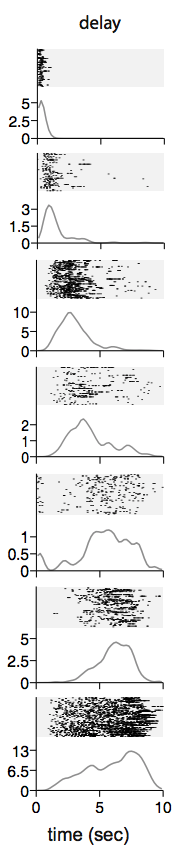
\includegraphics[width = \linewidth]{figs/MacDetal11.png}
	\end{minipage}
	\begin{minipage}{.28\linewidth}
		\textbf{b}
		\begin{center}
				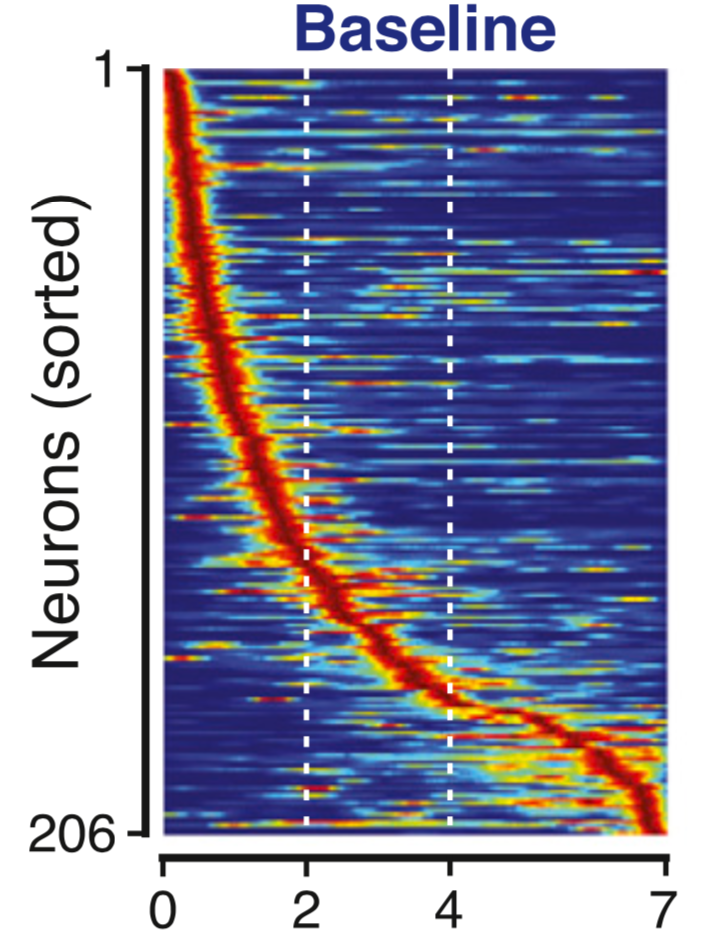
\includegraphics[width =\linewidth]{figs/RobiEtal17.png}
				%CA1 Rat
				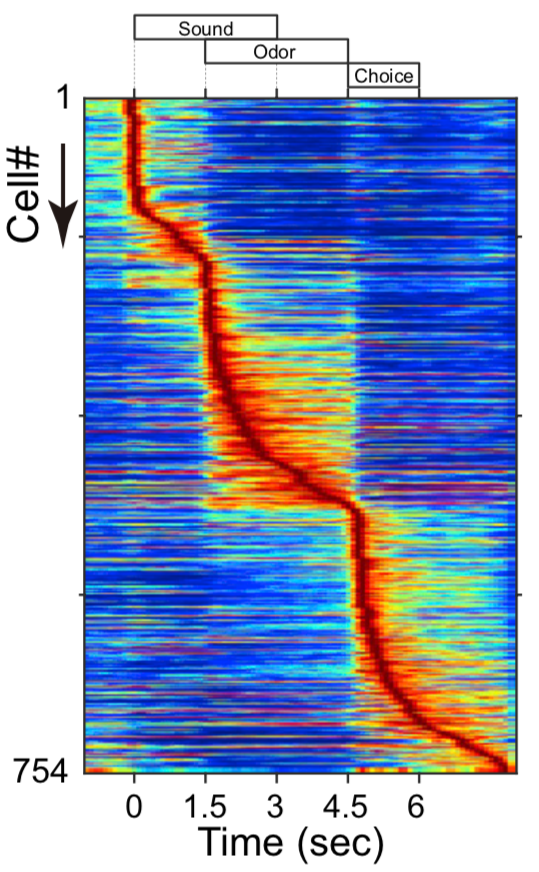
\includegraphics[width =\linewidth]{figs/TeraEtal17.png}
				%CA1 Rat
		\end{center}
	\end{minipage}
	\begin{minipage}{.51\linewidth}
		\begin{minipage}{.49\linewidth}
			\begin{center}
				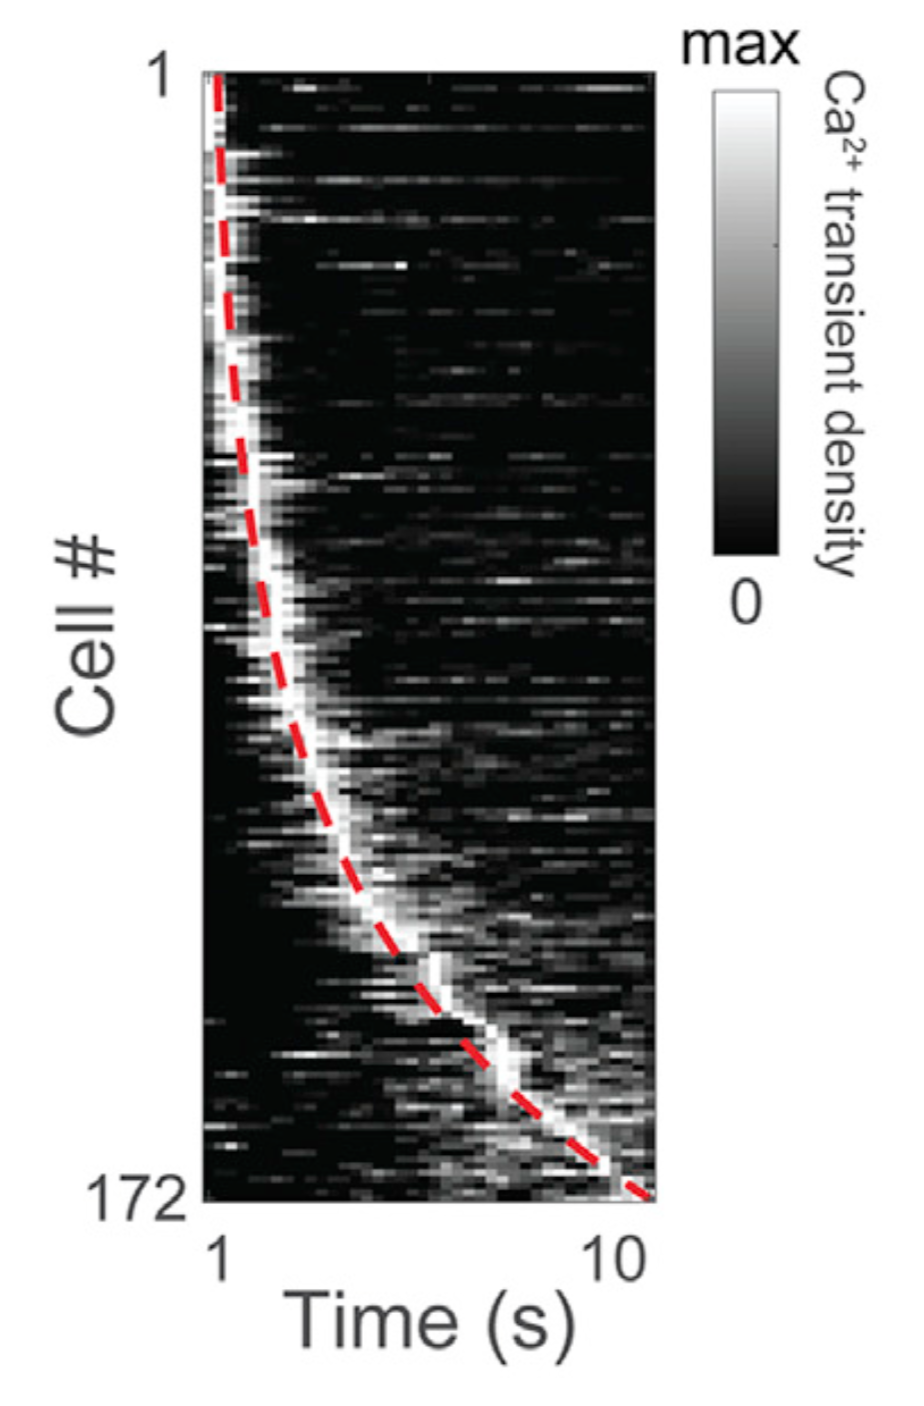
\includegraphics[width = \linewidth]{figs/MauEtal18.png}
			\end{center}
			\end{minipage}
			\begin{minipage}{.49\linewidth}
				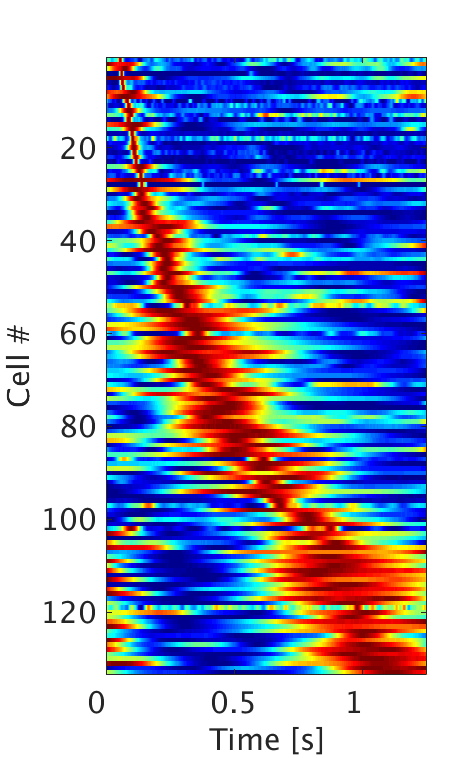
\includegraphics[width = \linewidth]{figs/HPC_Cruzado_Stretched_longer.png}
				%Monkey Hippocampus
			\end{minipage}
			\begin{minipage}{\linewidth}
				\textbf{c}
				\begin{center}
					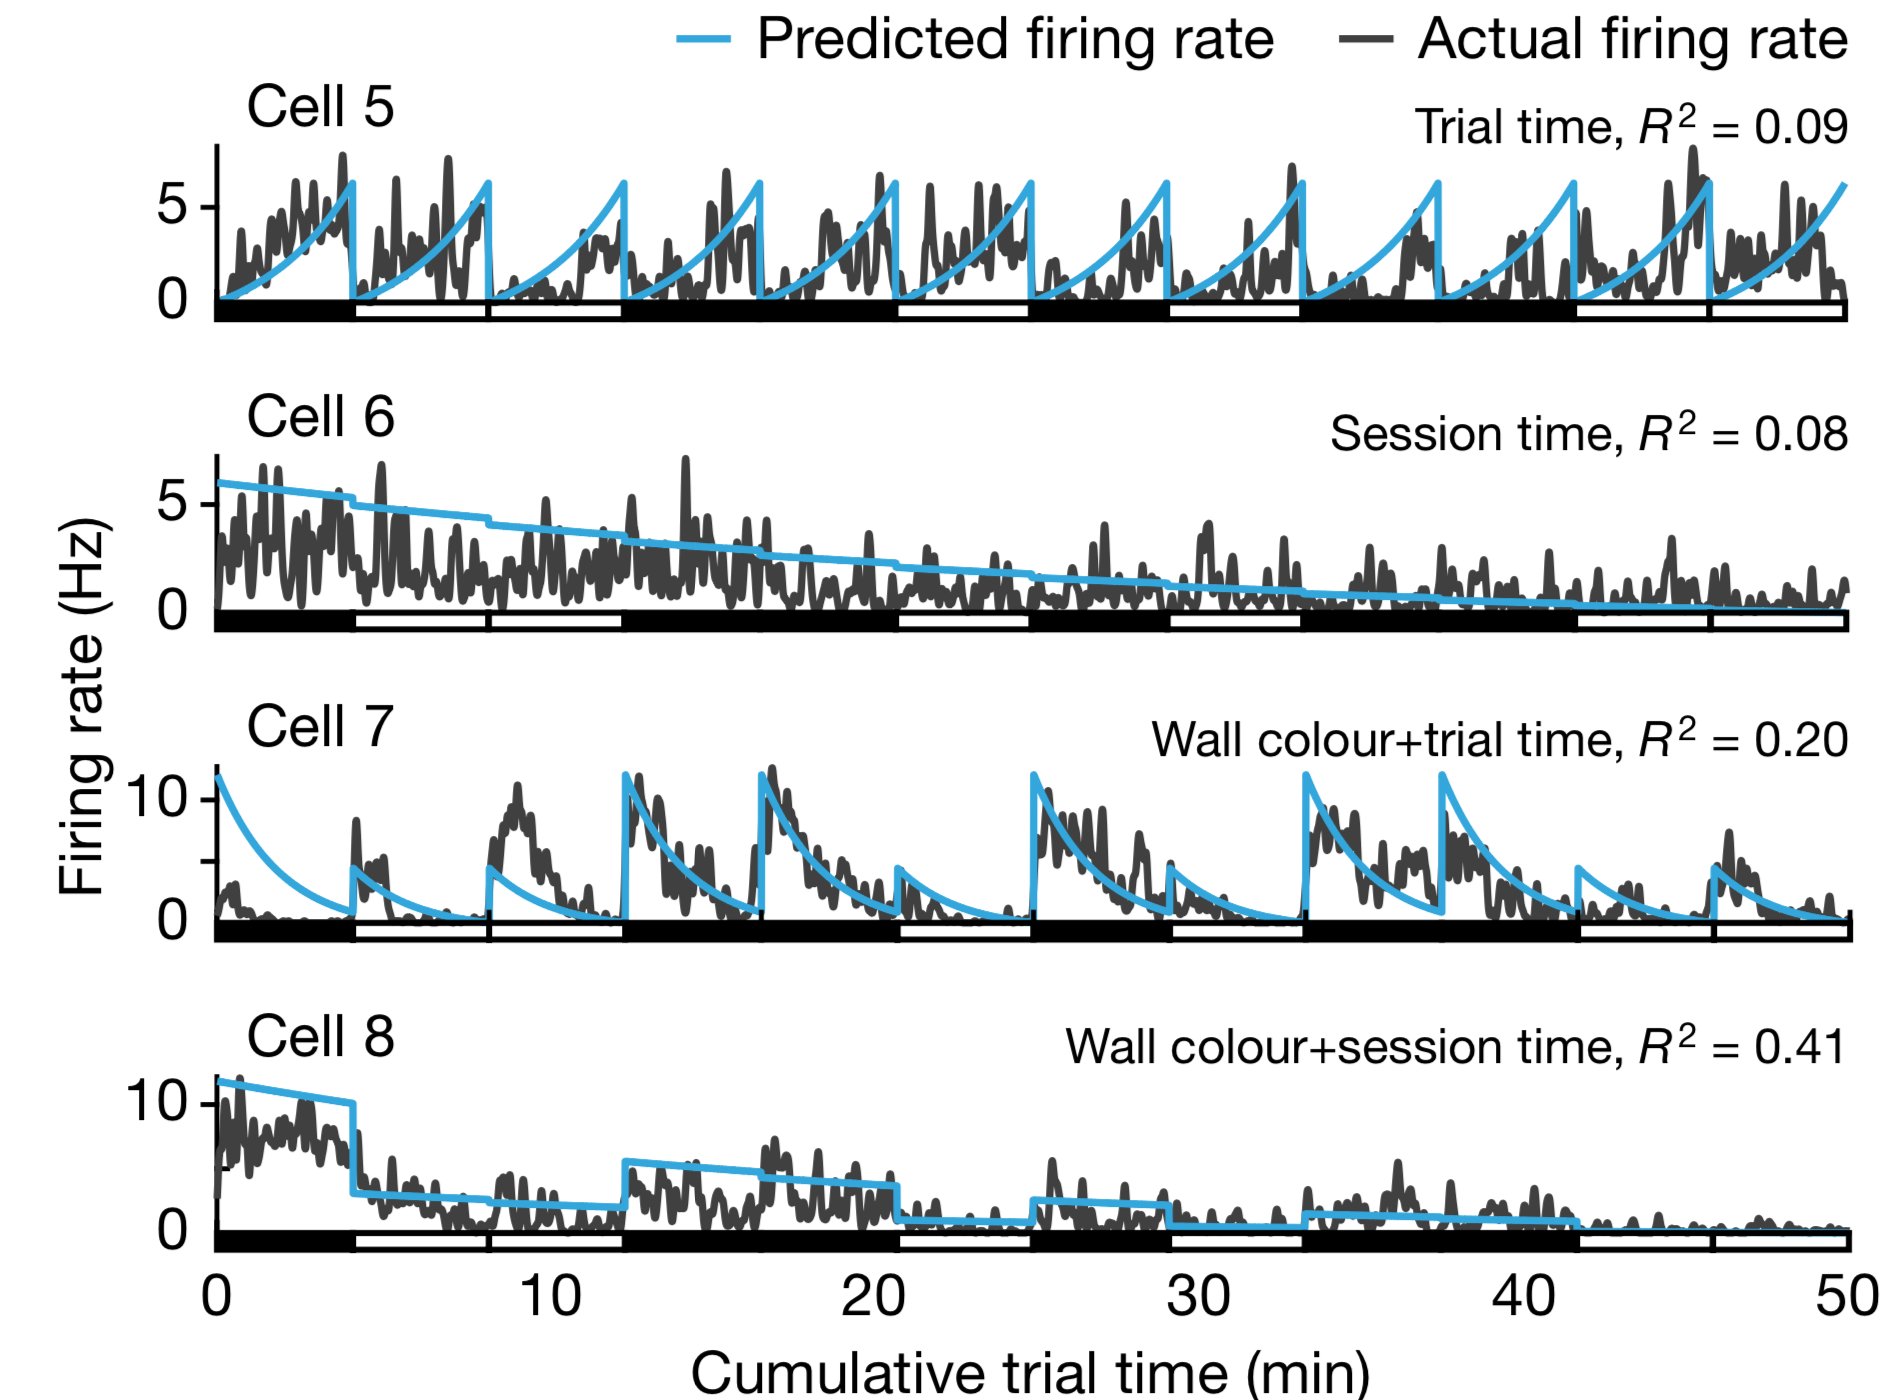
\includegraphics[width = \linewidth]{figs/TsaoFig.png}
					%LEC Rat
				\end{center}
			\end{minipage}
		\end{minipage}
	\end{minipage}
	\caption{
		\label{fig:TimeCellExamples} 
		\textbf{Coding of Time in the Medial Temporal Lobe.} \textbf{a},
		Rasters of sequentially activated time cells in rat hippocampus.  Time
		cells have receptive fields in time.  These fields widen the later a
		cell fires in the sequence (MacDonald et al., 2011). \textbf{b},
		Sequentially activated time cells have been observed in rodent and
		primate hippocampus. 
		Each plot shows the firing rate of a population of units as a function
		of time during a delay interval.  Each row is the firing field of one
		unit and the units are sorted according to their peak time.
		Time cells preferentially represent the beginning of the interval,
		resulting in a characteristic hook when the units are sorted as a
		function of their peak time. Firing fields later in the delay are
		also wider.  Both of these properties result in lower accuracy in the
		code for the time of an event with the passage of time (top row:
		Robinson et al., 2017; Mau et al., 2018; Cruzado et al., 2018, bottom
		left:  Terada et al., 2017).  
		\textbf{c}, Recent recordings from rat lateral entorhinal cortex do
		not show sequentially activated time cells, but rather cells that
		begin firing shortly following an event and exponentially return to
		baseline firing rates. (Tsao et al., 2018) 
	} 
\end{figure}

\nocite{MacDEtal11,RobiEtal17,TeraEtal17,MauEtal18,CruzEtal18,TsaoEtal18}

\begin{figure}
	\centering
	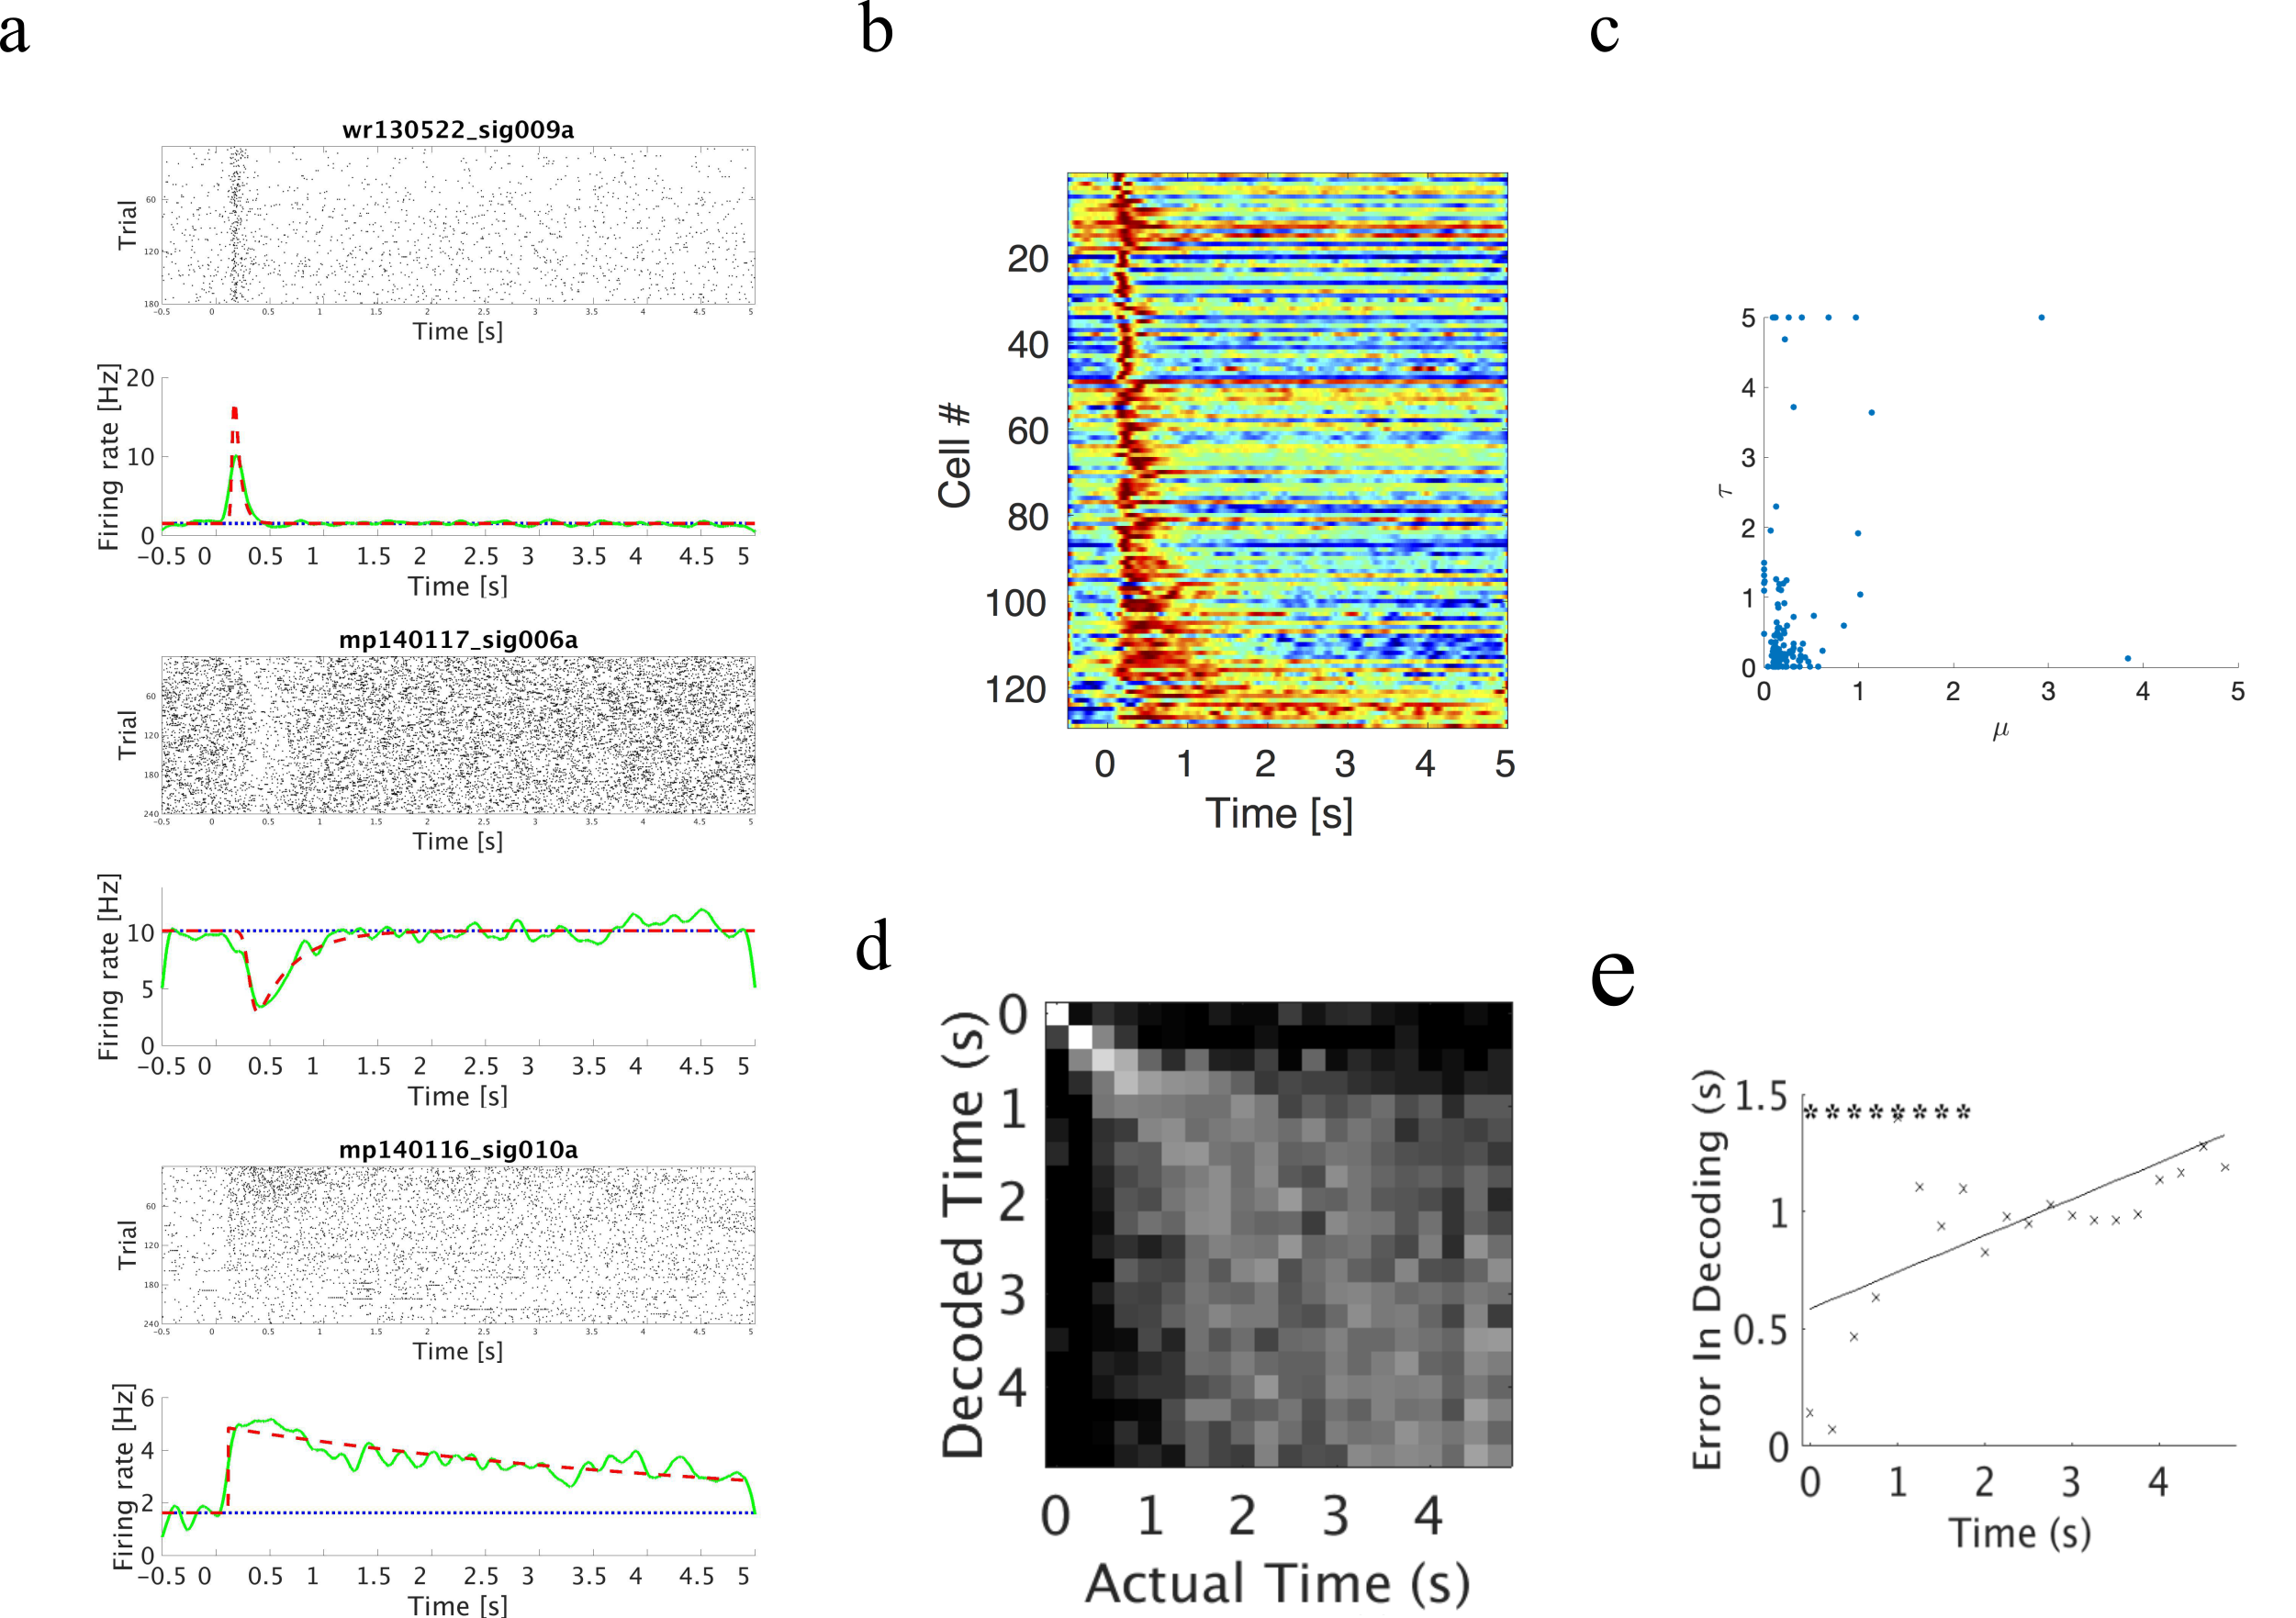
\includegraphics[width=1\textwidth]{figs/TemporalContextCells.png}
		\caption{
			\textbf{Temporal context cells in entorhinal cortex respond to the
					presentation of an image, then relax with a variety of
					rates, carrying information about time since the image was
					presented.
			}
			\textbf{a}, Three representative entorhinal units that changed their
			firing when an image was presented. In each plot, the trial raster
			is shown relative to the onset of
			each image. The bottom plot shows the the trial averaged firing
			rate (solid green line) and model estimate of the time course (red
			dotted line).  
			Many more example units can be found in Supplementary
			Figure~\ref{fig:MoreTCC}.
			\textbf{b}, Trial averaged, normalized firing rates
			of all entorhinal units that changed their firing when the image
			was presented, sorted by their time constant.  The majority of
			units responded shortly after image presentation.  Many units
			relaxed back to baseline quickly, but some relaxed more slowly.
			Across units the population showed a spectrum of decay rates.
			\textbf{c},  Joint distribution across units of parameters $\mu$, an
			estimate of peak time, and $\tau$, an estimate of 
			relaxation time.  Values of
			$\mu$ were clustered around a few hundred~ms whereas values of
			$\tau$ spanned the full 5~s of image presentation.  \textbf{d},
			Time since presentation of the image could be decoded from the
			population of entorhinal units.  A linear discriminant analysis
			(LDA) decoder was trained to decode time and then tested on
			left-out trials.
			The x-axis indicates the actual time bin which the LDA attempted
			to decode  The y-axis indicates the decoded time and the greyscale
			gives the log of the posterior probability.  Perfect decoding
			would result in a white diagonal.  Uniform decoding would result
			in a grey square.   The broad diagonal structure in the empirical
			results show that decoding is better than chance and decreases in
			precision with the passage of time.
			\textbf{e}, The average absolute value of decoding error increases
			with time.  Decoding error is the absolute difference between the
			decoded time and actual time.   The decoding error goes up with
			time, as shown by the fitted regression line (black line).  The
			asterisks mark time bins for which the significance level of the
			decoding accuracy has been further verified.  
			\label{fig:SingleCellResults}
	}
\end{figure}


\section{Results}


A total of 349 units were recorded from the entorhinal cortex in 2~macaque
monkeys during performance of a visual free viewing task.  Each trial began
with fixation, followed by presentation of a complex visual image that remained on the
screen for five seconds of free viewing.
Figure~\ref{fig:SingleCellResults}a  shows rasters and PSTH
(green dashed line) for
representative units.  Unlike canonical hippocampal time cells, which are
activated at a variety of points within the delay (e.g.,
Figure~\ref{fig:TimeCellExamples}a, b), most entorhinal units changed their firing
relative to background a short time after the presentation of the visual
stimulus.
While most of the responsive units increased their firing rate after the
stimulus was presented there were some units that decreased their firing rate
in response to the presentation of the picture.  Although behavior was not
controlled during the five second free viewing period, the response of these
neurons was consistent across trials (this can be seen by examination of the
trial rasters).

Although the image-responsive neurons in EC responded at about the same time
post-stimulus, they relaxed back to their baseline firing at different rates.
Whereas some neurons relaxed back to baseline quickly (top), some relaxed much
more slowly.  For instance the unit shown in the bottom of
Figure~\ref{fig:SingleCellResults}a has not returned all the way to baseline
even after five seconds.

\subsection{Quantifying temporal response properties}
We modeled each neuron's temporal
responsiveness relative to the onset of the visual stimulus based on previous
maximum likelihood methods for estimating time cell activity
\cite{TigaEtal17}.  This method is described in detail in the methods (see
especially Figure~\ref{fig:SMTschematic}c, d).
Because the goal of this analysis is to understand the distribution of
parameters across units, it is desirable to minimize the noise in the
parameter estimates.  To this end we used a very conservative criterion to
identify temporal context cells (see methods for details). 
This method identified 129/349 units as temporal context cells.
Of those 129 responsive units, 100 units showed an increase in their firing rate in response to
stimulus onset while 29 showed a decrease in their firing rate.

Figure~\ref{fig:SingleCellResults}b summarizes the temporal firing rate
properties of these 129 units.  Each row of the figure shows the deviation from
baseline of each unit over the course of a trial. %Still would be nice for a better description.
As can be seen from the figure, almost
all of the units reached their maximum deviation from baseline within a few
hundred milliseconds of the image presentation.  This is in contrast to
analogous plots for hippocampal time cells in which different units fire in
sequence tiling the delay (e.g., Figure~\ref{fig:TimeCellExamples}a, b).  The
variability across units in this entorhinal population is not in the time at
which the units reach their maximum deviation from baseline, but rather in the time
course over which each unit relaxes.  This can be seen in the progressive
widening of the ridge in Figure~\ref{fig:SingleCellResults}b from top to
bottom.  

The maximum likelihood method provides two key parameters that enable us to
quantify these properties.  The parameter $\mu$ approximates the time at which
each unit reaches its maximum deviation from baseline.  Another parameter
$\tau$ measures how long each unit takes to relax back to its baseline firing
rate (see Figure~\ref{fig:SMTschematic}d).
Figure~\ref{fig:SingleCellResults}c shows the values of these key
parameters for each unit that was categorized as a temporal context cell.  
The values of $\mu$ were clustered at small values.
The median value of $\mu$ was 160~ms, the interquartile range was 130~ms to
270~ms and .9 of the units had a value of less than 440 ms.
In contrast, $\tau$ showed a much wider distribution.  For
instance, several units had a $\tau$ of 5~s, the highest value 
considered given the five second free viewing period. 
The mean value of $\tau$ was 
750~ms with a standard deviation of 1300~ms.
The median value of $\tau$ was 210~ms, comparable to the value for $\mu$, but
the interquartile range was much broader, ranging from 90~ms to 640~ms and .9 of
the units had a value less than 1920~ms.  




Noting that the firing fields of hippocampal time cells spread out as the
sequence unfolds \cite{KrauEtal13,HowaEtal14,SalzEtal16}, to determine if this
property also held for temporal context cells, we examined the
relationship between $\mu$, an approximate measure of the time of peak firing 
of each unit and $\tau$, a measure of unit decay rate. 
The values of $\mu$ and $\tau$ measured for temporal context cells in
entorhinal cortex were not correlated with one
another as measured by a Kendall's $\tau$ correlation test, $\tau = .011$,
$p> .1$.  To assess whether this null effect is reliable, we computed the
Bayes factor, a measure of the likelihood of the null hypothesis.  This analysis
yielded a Bayes factor of $BF_{01} =8.537$, indicating strong support
that unit $\mu$ and $\tau$ values are uncorrelated. 
Unlike hippocampal time cells, there is no evidence that temporal
context cells that peaked later in the delay showed broader 
firing fields.  In contrast to hippocampal time cells, the overarching conclusion 
from these analyses is that the firing of entorhinal units deviated from background 
firing shortly after the presentation of the stimulus and then relaxed exponentially with a 
variety of time constants independent of peak time.


\subsection{Decoding time after image presentation from units in monkey
entorhinal cortex}

It is well-understood that sequentially-activated time cells can be used to
decode the time since the beginning of a delay \cite<e.g.,>[Supplementary
information, Figure~\ref{fig:LDA_simulated}]{MauEtal18}.  The accuracy of the
temporal decoding can be used to assess the temporal information present.
From a theoretical standpoint, we would expect exponentially decaying cells to
have temporal information, but to have less information present as time
elapses (see simulated data analysis in Supplementary information,
Figure~\ref{fig:LDA_simulated}).  A linear discriminant analysis (LDA) was
used as the decoder to test this hypothesis.  In this analysis the LDA
classifier was trained on the firing rate across units at each of several time
bins for a subset of the trials (see Methods for details).  To evaluate the
amount of information about time available in the population, the classifier
was then used to predict the time bin for time bins from a different subset of
trials.  To the extent the predicted time bin is close to the actual time bin,
one can conclude that the population response carried information about time.


\subsubsection{Time was decoded better than chance}

Figure~\ref{fig:SingleCellResults} shows the results of the LDA on the units from
monkey entorhinal cortex. Our first question was whether or not the population
of temporal context cells contains information about time.
The confidence of the decoder, the posterior
distribution, is shown for each actual time bin vs. decoded time bin in
Figure~\ref{fig:SingleCellResults}d).  Perfect prediction would correspond to a
bright diagonal, random uniform decoding would correspond to a gray square.
Qualitatively, the non-uniformity of Figure~\ref{fig:SingleCellResults}d suggests
that elapsed time can be decoded from the entorhinal population.  To
quantitatively assess this, we found that the posterior distribution from the
test data was reliably different from a  uniform distribution using a
chi-squared goodness of fit test, $\chi^2(X) = 522.17$, $p<.001$.  

As an additional test to evaluate whether the population of temporal context
cells contains information about time, we computed the mean absolute value of decoding
error from the cross-validated LDA.
To quantitatively compare this value to chance we compared the true value of decoding error
to the distribution of decoding errors across a permuted data set.  In each of
1000~permutations we randomly assigned the time bin labels of the training
events used to train the classifier.  The observed value of the absolute value of the decoding error
was 1.35~s, which is less (i.e., more accurate) than the mean absolute value of the decoding error for all 1000
permutations (shown in Figure \ref{fig:permutest}, normally distributed with mean 1.66~s, with standard deviation .04~s, $p<.001$ that 1.35~s comes from this distribution).  These analyses show that time can be decoded from monkey
entorhinal cortex.

\subsubsection{The precision of the time estimate decreased as the interval
unfolded}

Although the population response in entorhinal cortex could be used to
reconstruct time, inspection of Figure~\ref{fig:SingleCellResults}\textbf{d} suggests
that the precision of this reconstruction was not constant throughout the
interval.  Figure~\ref{fig:SingleCellResults}\textbf{e} shows the average absolute
value of the decoding error at each time bin.  As can be seen from the
figure, this error
increased as a function of time.  A linear regression of decoding error as a
function of time showed a reliable slope (slope of $.18\pm.04$, intercept $.5\pm.1$, $p < .001$, $R^2=.56$, 18 Error degrees of freedom).  
Thus the temporal information decreases as time elapses.

\subsubsection{Time can be decoded out to at least 1.75 seconds}
To assess how far into the interval time could be reconstructed, we repeated
the LDA analysis excluding progressively more time bins starting from zero.
If the LDA can reconstruct time using only bins corresponding to times $\geq
t$, then we can (conservatively) conclude that time can be reconstructed at
least time $t$ into the interval. To assess this quantitatively, the
the actual data was compared with permuted data for each repetition of the LDA.  
The mean of
the absolute error across time bins can be used as a metric to compare the
performance of the LDA on permutations of the data against its performance on
the actual data (see Methods for more details). This permutation testing suggests that time can be decoded up to at least 1.75
seconds from stimulus onset.  Thus the population of temporal context cells
contains information about time long after the median value of
the peak time (160~ms).




\subsection{The population of EC units changes slowly, on the scale of
minutes}

The above results show that the population of EC units showed consistent
changes in firing on the scale of seconds. Previous work by \citeA{TsaoEtal18}
showed units that relaxed over much longer time scales ranging from minutes to hours,
such that the population was able to encode temporal information over
long time scales. In order to measure whether an analogous slow change
also existed in monkey EC, we examined changes in activity across trials.
Visual inspection of unit rasters revealed numerous cells that changed their 
firing rate over the course of the session (Figure~\ref{fig:Rec}a).  
This pattern was observed for both visually responsive units
and units that were not visually responsive. 
In order to determine which cells showed a slow change in firing, 
we fit the time series of unit firing during a recording 
session with a first order autoregressive model. 94/349 units were significantly fit 
by the model, of which 40/94 were temporal context cells. We then calculated how
long the 94 units remained significantly autocorrelated. 
As seen in Figure~\ref{fig:Rec}b
the units showed a spectrum of significant autocorrelations.
This suggests that individual units in EC systematically change
their firing pattern at different rates at longer time scales as well. 
At the population level, we compared the cosine similarity of 
simultaneously recorded units during first presentation 
trials as a function of the
recency between trials within the same block.  
For a given image, the image presented just
before would have a recency of~1,
the image two before that would have a recency of~2 (Figure~\ref{fig:Rec}c, top). 
Figure~\ref{fig:Rec}c, bottom shows a robust effect of recency on population
similarity.
This impression was confirmed by a linear mixed effects regression, $t(1796)=-12.01$, $p <0.0001$. This
suggests that the population of monkey EC also shows gradual changes on the scale of
minutes.

\begin{figure}
\begin{tabular}{l l l}
\textbf{a}\\
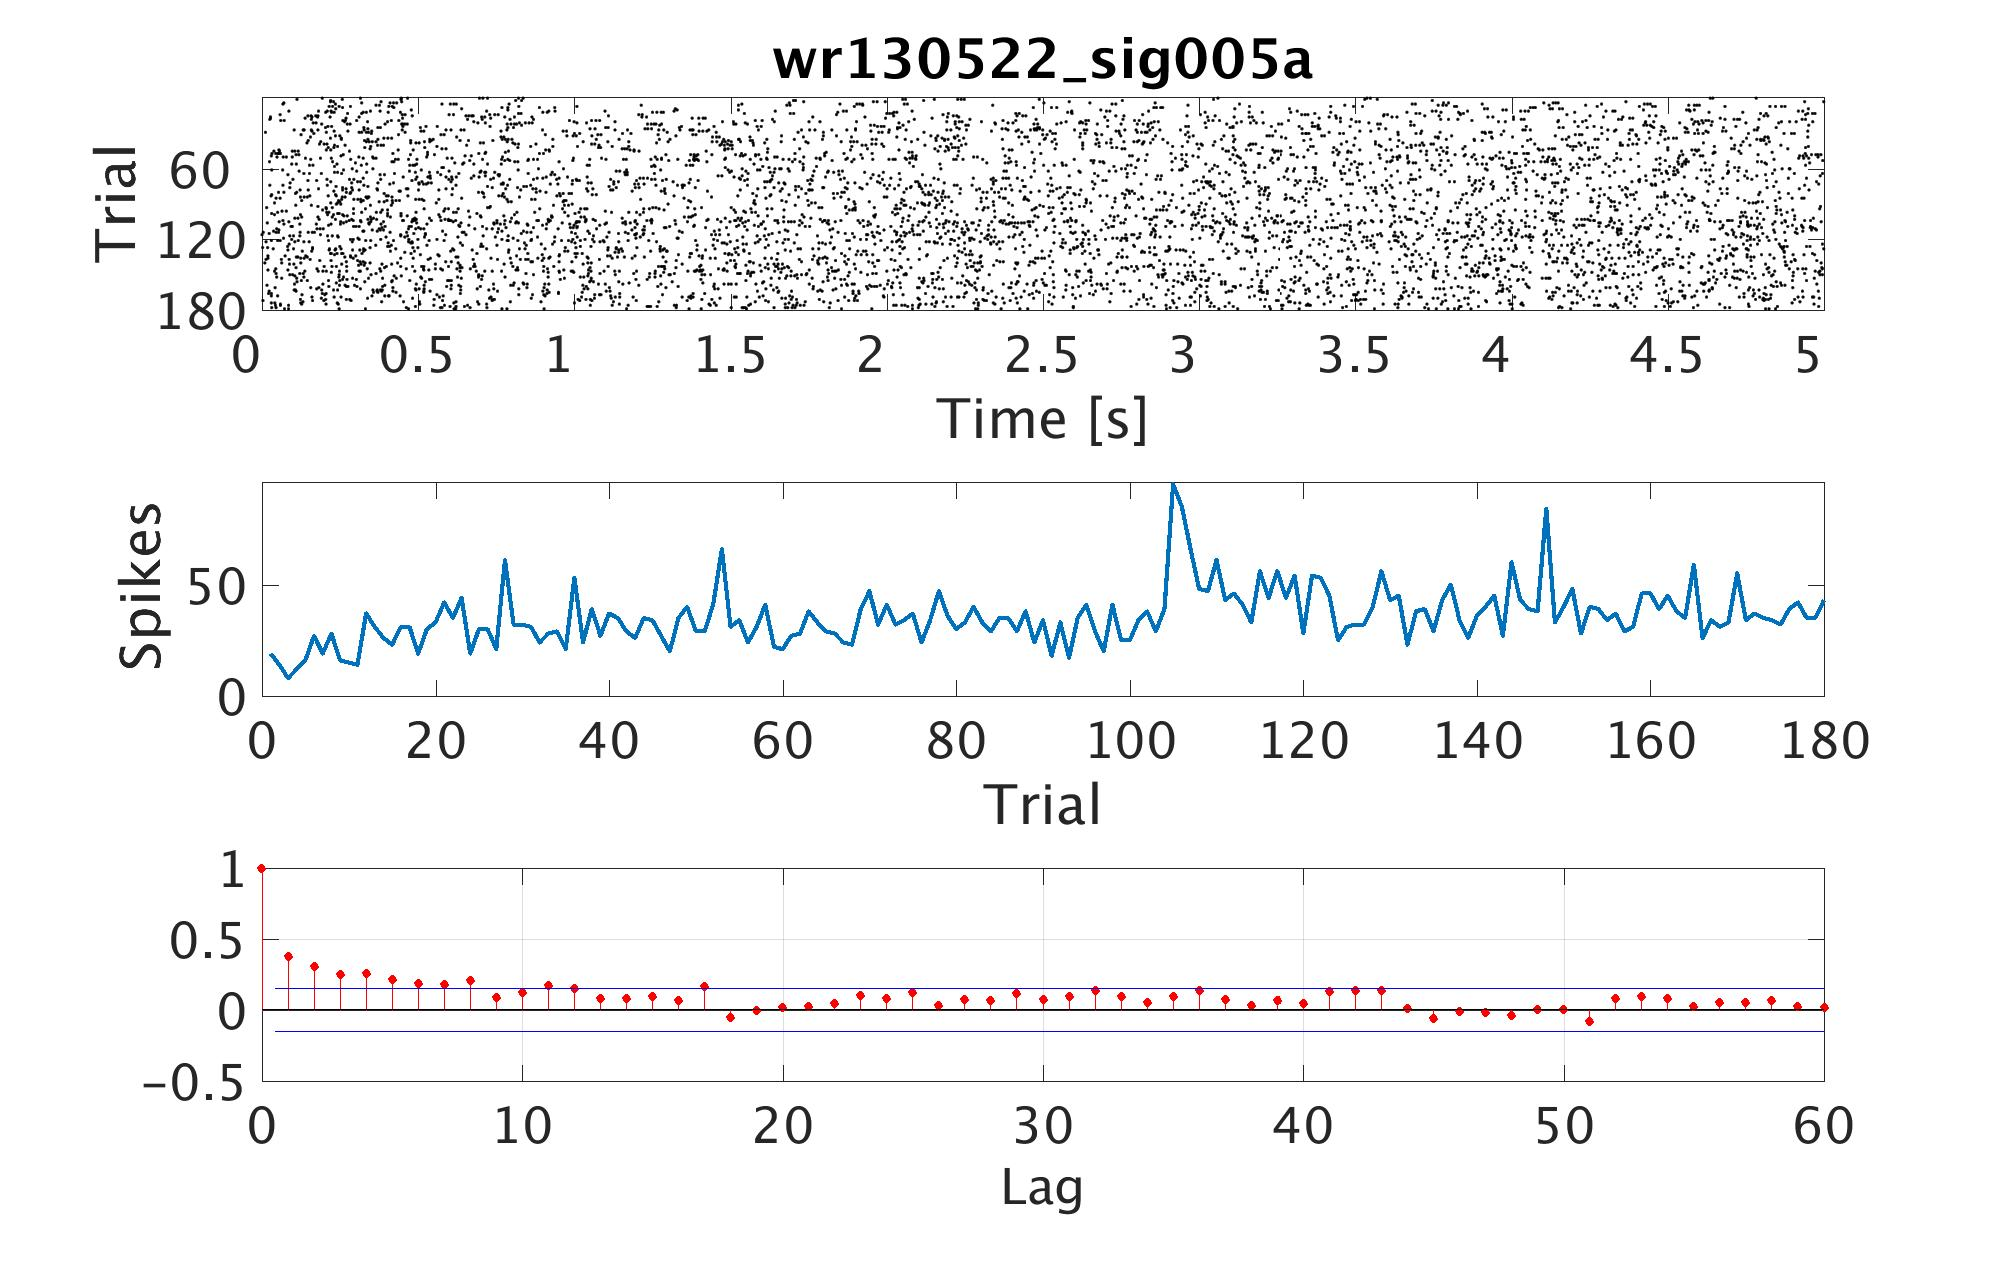
\includegraphics[width =.33\textwidth]{figs/cutAR_Rec_139_v_11.jpeg}
&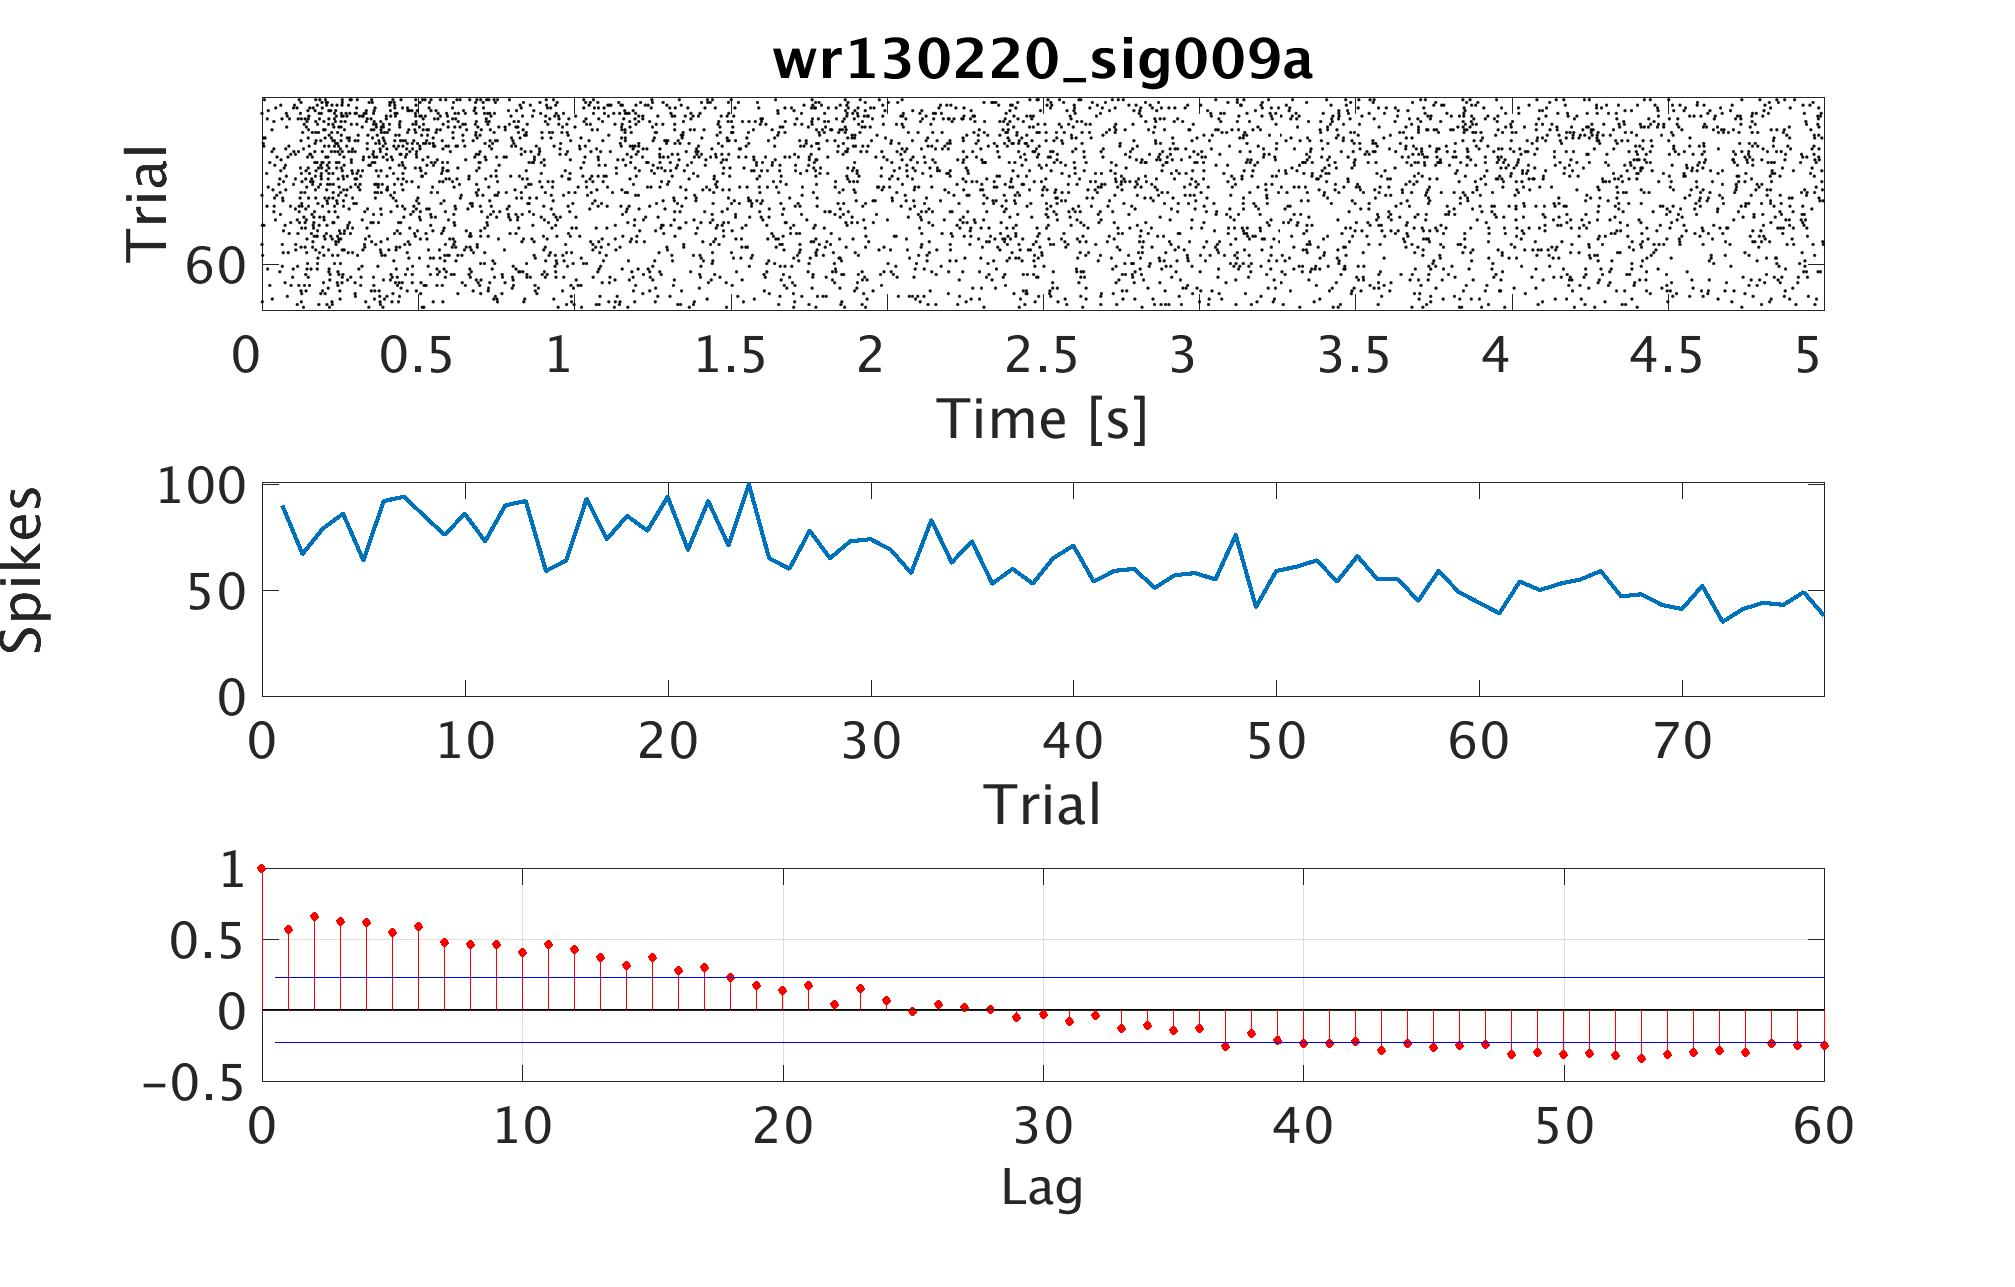
\includegraphics[width =.33\textwidth]{figs/cutAR_Rec_69_v_11.jpeg}
& 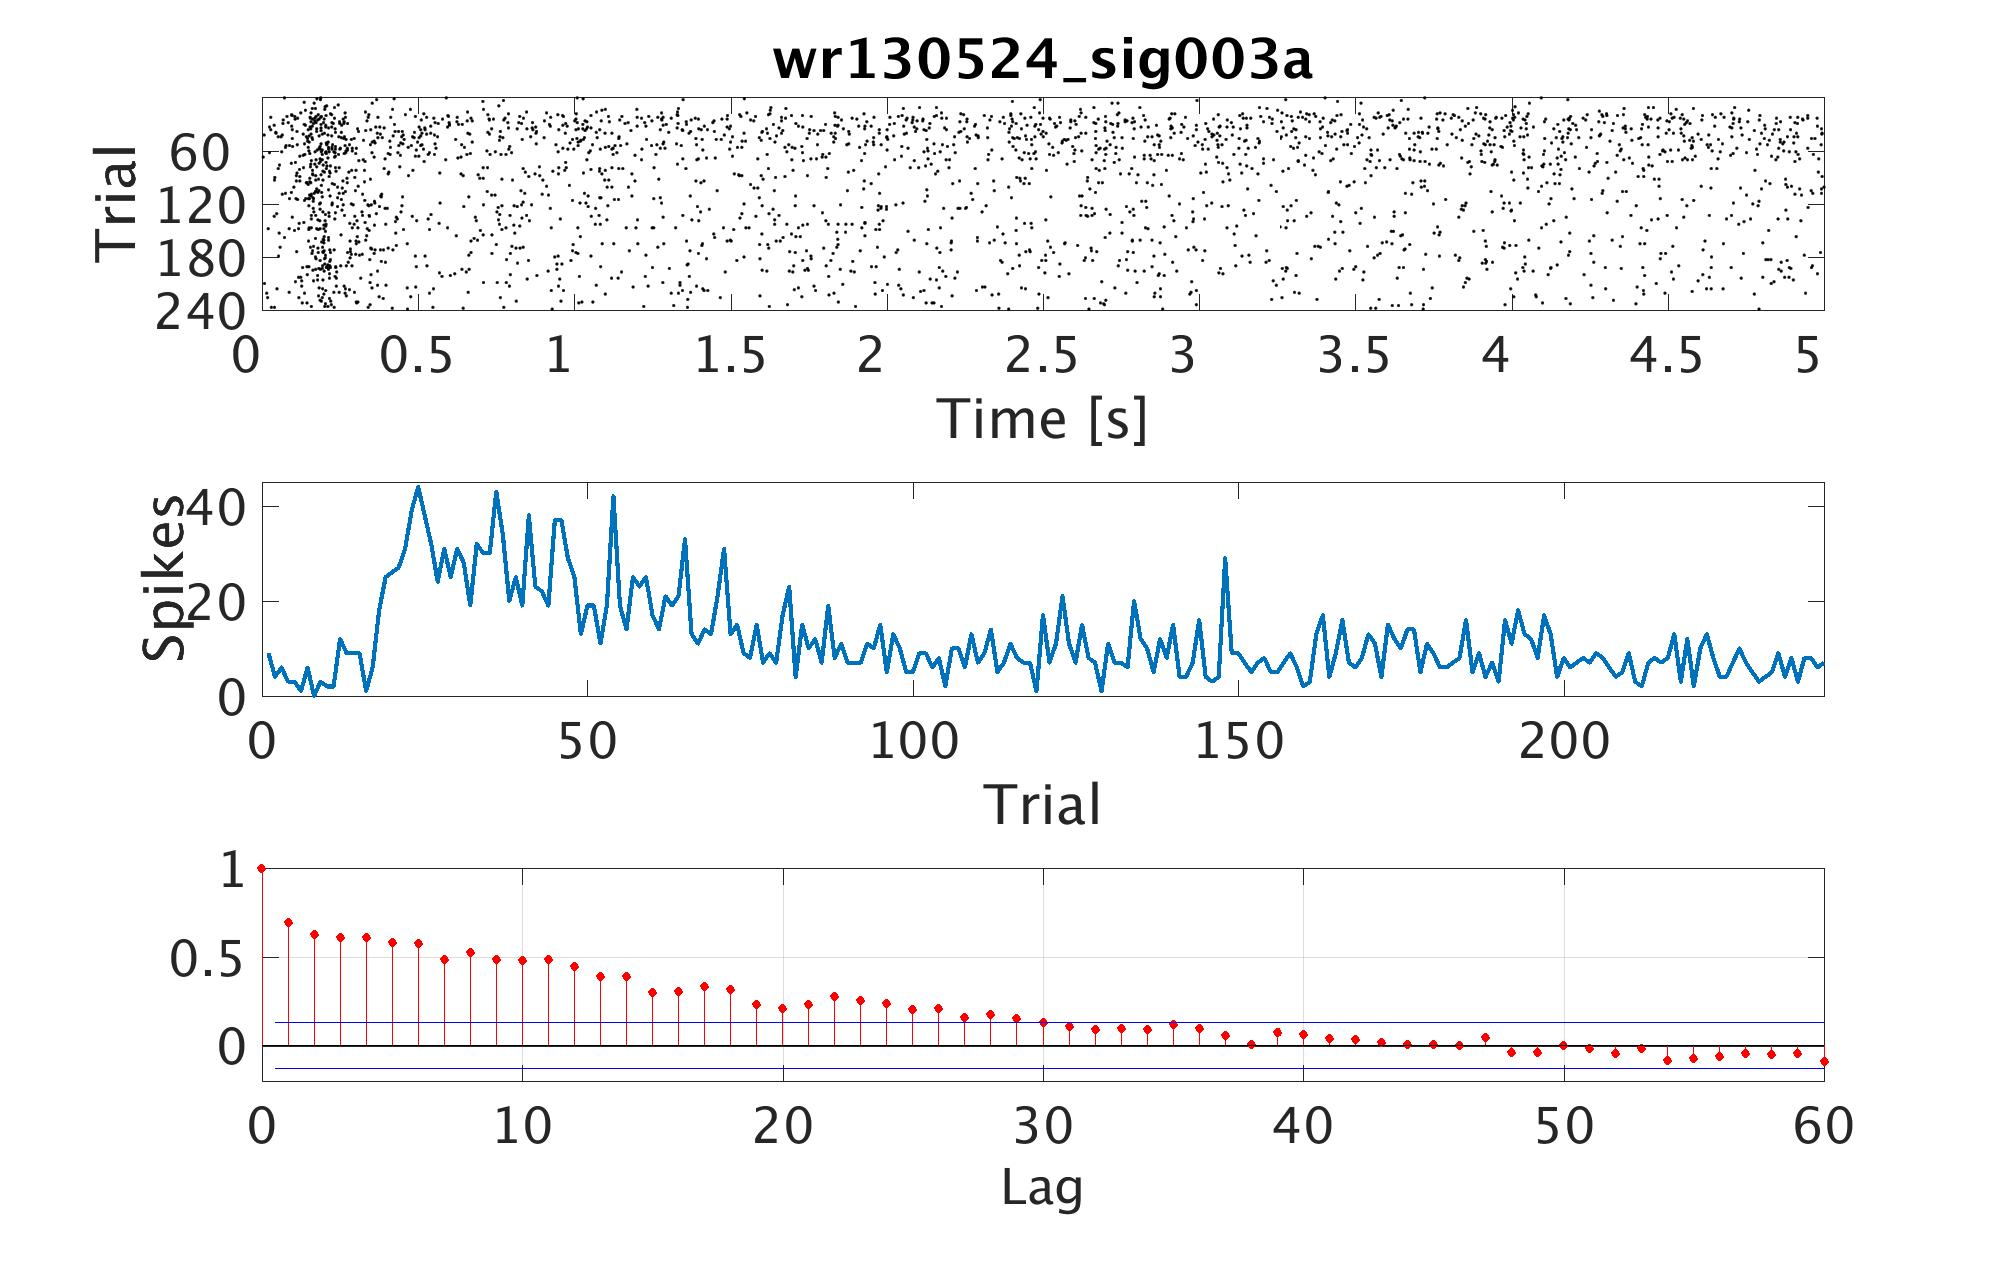
\includegraphics[width =.33\textwidth]{figs/cutAR_Rec_149_v_11.jpeg}
\\  
\end{tabular}
\begin{tabular}{l l }
\textbf{b}  
&\textbf{c} \\

\includegraphics[width=.48\textwidth]{figs/EmptyWhiteSpace.png}
&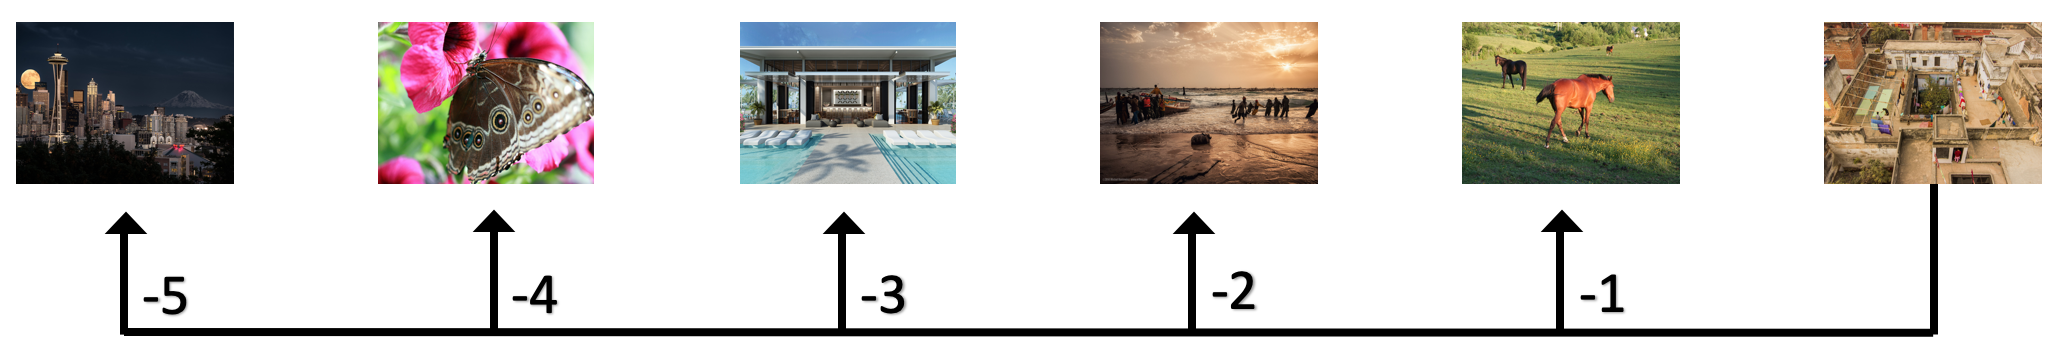
\includegraphics[width=.48\textwidth]{figs/RecS.png}\\
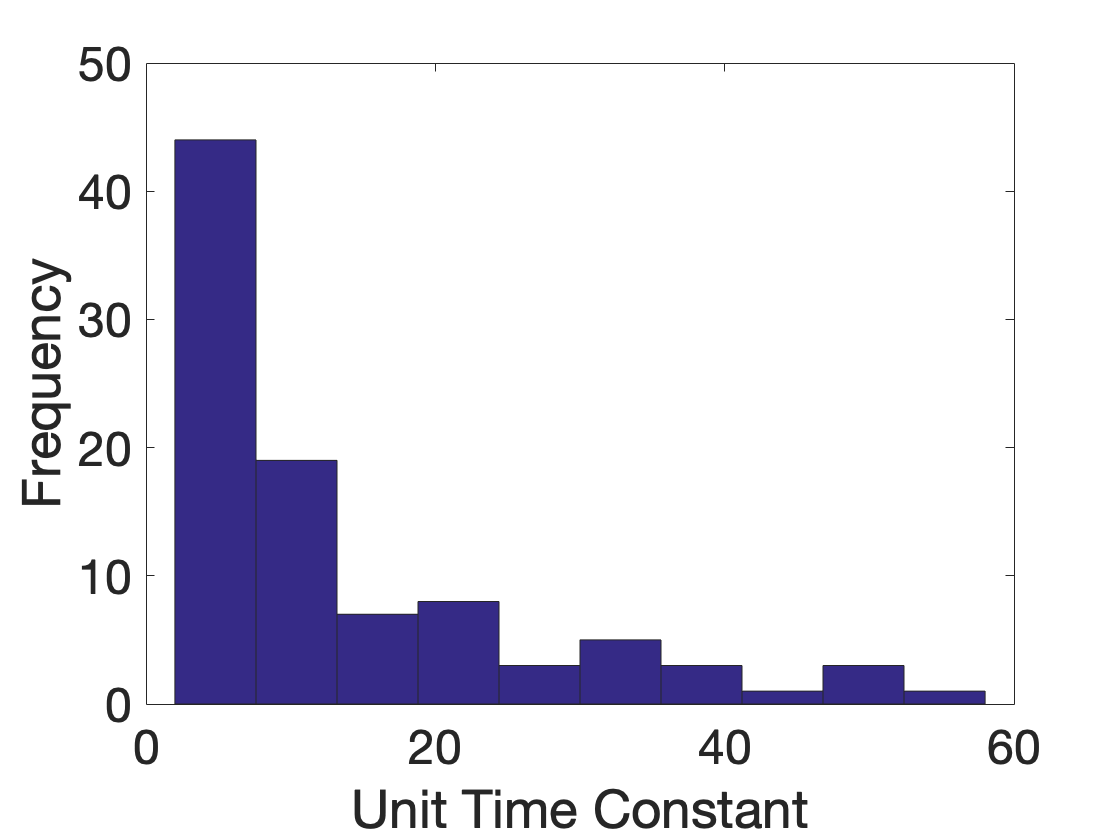
\includegraphics[width =.48\textwidth]{figs/AutoCorrDist.png}
&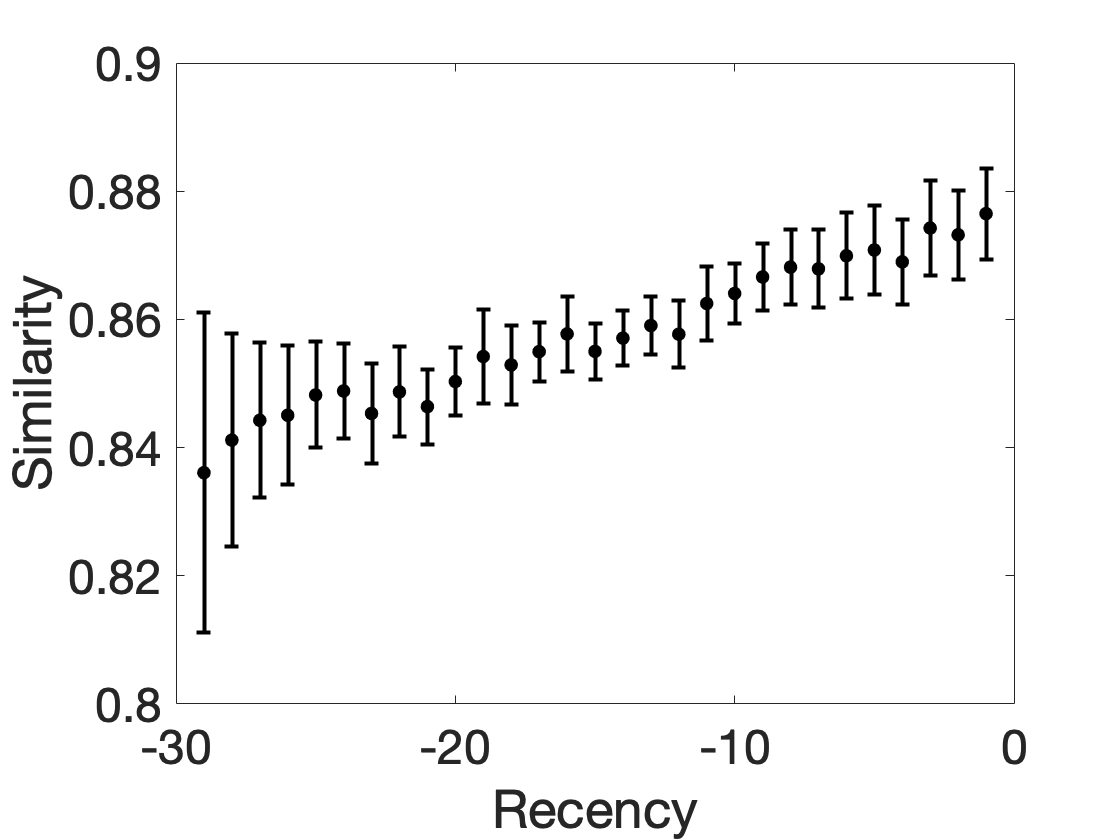
\includegraphics[width = .48\textwidth]{figs/Rec.png}
\end{tabular}
\caption{ \textbf{In addition to coding time on the scale of seconds, the
entorhinal population changed gradually over minutes with different units
changing at a wide variety of rates.}
\textbf{a}, Many units appeared to change their firing rate
systematically over the course of an entire session.   In each plot the top
panel shows the trial raster aligned to presentation of the image with the
first trial at the top.  The middle panel shows the number of spikes in the
five second interval as a function of trial number.  The bottom panel shows
the autocorrelation function over trials. We defined the macrotime constant
as the largest lag over which the autocorrelation function was above chance.
These three units show a variety of macrotime constants from short to long
(left to right).  The middle and right units were also classified as temporal
context cells based on their responsiveness to the image on the scale of
seconds.
\textbf{b}, The distribution of macrotime constants for units that were
autocorrelated across trials, as assessed by an AR(1) model.  There was a
broad spectrum of macrotime constants, with a peak near short times and
extending to many dozen trials.  Each trial is separated by X seconds, so this
corresponds to about Y.
\textbf{c},  To quantify the drift in the ensemble at the population level, we compared
the similarity of the population response as a function of  \emph{recency}.
Here recency measures the difference in trial number 
when two  population vectors across the five second interval were measured.  A
recency of~1 compares the population vector from a trial to the preceding
trial.  The cosine similarity between population vectors
changed robustly as a function of recency, meaning that the firing
rate of neurons in entorhinal cortex changed slowly across many  trials.
\label{fig:Rec}
} 
\end{figure}

\subsubsection{Firing of EC units was similar for presentations of the same
image}

In this experiment, each image was presented twice.  Although it is not
practical to assess image coding using a classifier, it is possible to exploit
the repetition of images to determine if entorhinal cortex units contained
information about image identity. 
One possible measure of how the population encoded items 
is to determine how correlated each unit's spiking activity was during the first and
second presentation of images using Kendall's $\tau$, a measure of correlation
that is appropriate for non-normal data.
If units respond to stimulus identity, spiking activity should show a positive correlation
for identical images.
The distribution of correlation coefficients across
units resulted in a mean that was significantly 
greater than zero, $t(303)=6.43$, $p <0.0001$,
$\text{ Cohen's } d = 0.3687$, indicating that the 
population's spiking activity was
similar during first and second presentations of items
(Fig.~\ref{fig:StimInfo}a). This was confirmed by a Wilcoxon signed rank
test, a test that does not assume normality $V = 32931, p <0.0001$.
Further, temporal context cells resulted in
a distribution of correlation coefficients with a mean significantly greater
than zero, as measured by t-test $t(118)=5.10$, $p <0.0001$, $\text{ Cohen's } d = 0.4677$
and Wilcoxon signed rank test, $V = 5659, p <0.0001$.
 While units that were not fit also resulted in a distribution with a mean
significantly different from zero $t(185)=3.65$, $p <0.01$,$\text{ Cohen's } d
= 0.2673, V = 11270, p = 0.0001$ these two distributions were also significantly
different from each other by t-test $t(303)=2.25$, $p =0.02$,$\text{ Cohen's } d = 0.2253$,
Wilcoxon rank sum test $V = 9092, p = 0.01$
and permutation analysis 98607/100000. 
Taken together, this suggests that EC unit spike activity
contains information about stimulus identity.


\subsubsection{The population of EC units was more similar during image repetition}

At the individual unit level, EC responds to stimulus identity.  
If the response of the entire population contained information about stimulus
identity, we would expect, all things equal, that the population vectors 
corresponding to presentations of the same image would be more similar 
than the population vectors corresponding to presentations of different images.
It is well-known that repeated presentations of a visual image result in less
neural firing than initial presentations \cite{BrowAggl01,MeyeRust18}.  To
control for the repetition effect these analyses compared the similarity
between initial presentation of an image and second presentation of the same
image to the similarity between second presentations of an image and
repetitions of a different first presentation image. 
Figure~\ref{fig:StimInfo}a shows the results of a population analysis 
comparing the similarity of the ensemble response to the second presentation
of a target image and first presentations of the same image (lag~0) and to
first presentations of neighboring images.  Images that followed the initial
presentation of the target image are associated with positive lags.  For
instance, lag $+1$
corresponds to the image that followed the presentation of the target image;
lag $-1$ corresponds to the image that was presented just before the
target image.  As can be seen from Figure~\ref{fig:StimInfo}b, the similarity
to lag~0 was greater than adjacent lags.  
Statistical comparisons to lags $\pm 1$ each showed a reliable difference.
A within block mixed effects regression found that image repetition resulted in a statistically reliable
increase in population similarity $t(3758) = 3.59$, $p<0.001$, in addition to an
increase in similarity for items presented closer together $t(3758)=8.37$, $p<0.0001$. 
A post-hoc paired t-test comparing population similarity at the block level showed that
similarity at lag~0 was reliably larger than at lag $+1$, $t(63)=5.11$, 
$p<0.0001$, Cohen's $d = 0.61$, and lag $-1$, 
 $t(63)=5.02$, $p<0.0001$, Cohen's $d = 0.60$. 
To evaluate the same hypothesis using a non-parametric method, we performed a
permutation analysis by randomly swapping within-session pairs of lag~0 and lag~$\pm 1$
and calculating the mean difference between the pairs 100000 times. 
The
observed value exceeded the value of 100000/100000 permuted values
for both lags $+1$ and $-1$. 


\section*{Discussion}


Episodic memory requires information about both the content of an event as
well as its temporal context \cite{Tulv83,EichEtal07,Eich17a}.  
Many units changed their firing in response to the onset of the visual image.
These \emph{temporal context cells} changed at about the same time within a
few hundred milliseconds after the image was presented.  However, temporal
context cells  relaxed back to baseline at different rates (see
Figure~\ref{fig:SingleCellResults}).  Information about time was implicitly
encoded in the slowly  relaxing firing rates allowing us to decode the time
since image onset over a few seconds (see Figure~\ref{fig:SingleCellResults}d-e). 
Notably, the relaxation rate was not constant across units, but rather
showed a spectrum of time constants.
In addition to temporal information on the scale of seconds, the population
also drifted over minutes (see Figure~\ref{fig:Rec}).
The population vectors following repeated presentations of the same image were
more similar to one another than to presentations of different images.   This,
coupled with several control analyses, enable us to conclude that entorhinal
units also carried some information about stimulus identity.  
Thus, entorhinal units had properties consistent with a temporal
record of the past constructed from a spectrum of time constants.  Because
this record contains information about what happened when, it could  be
helpful in supporting episodic memory.


Sequentially-activated time cells, such as have been observed in the
hippocampus \cite{PastEtal08,MacDEtal11,SalzEtal16}, medial entorhinal cortex
\cite{KrauEtal15} and many other brain regions
\cite{JinEtal09,MellEtal15,TigaEtal18a,TigaEtal17} also show a temporal record
of the past.
Although the entorhinal temporal context cells provided a temporal record of recent
events, they had different firing properties than time cells that have been
observed in the hippocampus and  other brain regions.   Different time cells convey the
past time of occurrence of an event by responding at different temporal lags
after the event.   Here the temporal context cells all responded at about the
same time but relaxed at different rates.  This result aligns well with
a recent report from rodent LEC \cite{TsaoEtal18}.  In that study LEC neurons
responded to a salient event---entering a new environment rather than onset of
a visual image---and then changed firing monotonically.  Notably, different
in that study, as in this one, different units responded at different rates.
The similiarity of these findings despite the many methodological differences
between the two studies---rats moving through a series of open enclosures
compared to seated monkeys observing a series of visual images---is striking.



\subsection*{Exponentially-decaying units with a spectrum of time constants is
just the Laplace transform of time}

This study and a previous rodent study \cite{TsaoEtal18} observed entorhinal
neurons that code time by gradually change their firing rate with different
units changing at different rates.  This is in contrast to the temporal coding
shown by time cells observed in the hippocampus and other regions.  Why would
the brain use two such distinct coding schemes to represent the same form of
information?
It has been proposed \cite{ShanHowa12,ShanHowa13,HowaEtal14} that the brain
estimates a temporal record of the past---a function over past time---by
first computing the (real) Laplace transform of that function.  
The Laplace transform of the
past with a discrete event would manifest as a set of exponentially-decaying
cells with a spectrum of time constants \cite{HowaEtal14}, very much like the
results observed here and in the \citeA{TsaoEtal18} study.  

Although it may seem inefficient to estimate the Laplace transform of a
function and then invert the transform rather than estimating the function
directly, there are several computational advantages to this approach.  For
instance, in much the same way that the Fourier transform has useful
computational properties that make it widely used in signal processing and
manipulation, many computations can be more efficiently calculated in the
Laplace domain \cite{HowaEtal16}.  The inverse transform, which takes a set of
exponentially-decaying temporal context cells into a set of
sequentially-activated time cells, can be implemented using simple
center-surround receptive fields in a feedforward circuit
\cite{ShanHowa13,LiuEtal18}.  Notably, one can use the same computational
framework to compute the Laplace transform of functions other than time,
including spatial variables \cite{HowaEtal14}, accumulated evidence
\cite{HowaEtal18} and temporal distance to expected outcomes
\cite{MomeHowa18}.  For instance, border cells observed in rodent and monkey
EC \cite{SolsEtal08,KillEtal12,HardEtal15}, have properties like one would
expect for the Laplace transform of distance to an environmental boundary.  In
the spatial case, the inverse transform of distance to a boundary would appear
as one-dimensional place cells
\cite{GothEtal96,LeveEtal09,BurgOKee96}.  Perhaps temporal
context cells and time cells---the Laplace transform and inverse transform of
functions of time---are a special case of a more general principle of
computational cognitive neuroscience. 




\section{Methods}

\subsection{Recording techniques}


357 cells were recorded in 2 macaque monkeys over 43 sessions. Of those cells,
349 were located in entorhinal cortex, 
while 8 were hippocampal cells and were
removed from subsequent analyses. 

\subsection{Behavioral task}


\subsection{Analysis of Neural Firing Fields}

Spikes were analyzed using a custom maximum likelihood estimation script run
in MATLAB 2016a. We calculated model fits across all trials. Fits were
compared using a nested maximum likelihood model of each cell's spike train. A
likelihood ratio test was performed to calculate the probability that
increasing parameters significantly improved a model's fit. This approach is
the same as the method used in \citeA{SalzEtal16} and other papers
\cite{TigaEtal17b,TigaEtal18a} to identify time cells. In the present paper, we
considered two models: a constant firing model and, in contrast to the
Guassian model used in the previous papers, we fit spikes to a
temporally-modulated convolution of a Gaussian distribution and exponential
distribution. The constant model,


\begin{equation}
M_1(t; \theta_1) = a_o
\end{equation}

consisted of a single parameter $a_o$ that predicted the probability of a spike at time $t$. The convolution model, 

\begin{equation}
M_2(t; \theta_2) =
\frac{p}{2}e^{\frac{\lambda}{2}(2\mu+\lambda\sigma^2-2t)}\text{erfc}(\frac{\mu+\lambda\sigma^2-t}{\sqrt{2}\sigma})+a_o
\end{equation}

where erfc is the complementary error function, consisted of five parameters,
the constant term $a_o$, a peak height term $p$, a decay rate $\lambda$ from the
exponential distribution, and $\mu$ and $\sigma$ from a Gaussian distribution
which describes the peak of the distribution and spread of the distribution
respectively. $\mu, \sigma, \text{and } \lambda$ are measured in terms of
seconds. $\mu$ and $\tau$ were allowed to take values between 0 and 5
\emph{s}. $\sigma$ was allowed to take values between 0 and 1 \emph{s}. Cell
fits were performed over a 5.5 \emph{s} window, encompassing 5 \emph{s} of
stimulus viewing and .5 \emph{s} of fixation prior to viewing. Kendall's
$\tau$ correlation coefficients and Bayes Factors were calculated using JASP
statistical software.

\subsection{Linear Discriminant Analysis}
\subsubsection{LDA Implementation in Matlab}
Time
was discretized into bins of 250~ms.  For each bin of each trial, the average firing rate was calculated.
Training and testing trials were separated by even and odd
trials.  The number of trials varied for each unit.  To mitigate any problems
from this, several steps were taken.  First, 4 units with less than 30~trials
each were entirely excluded from this analysis.  
Units with less than 200~trials were bootstrapped to 200~trials, while units
with more than 200~trials were randomly down-sampled.
To avoid errors due to a singular covariance matrix, a small amount of uniform
random noise ( between $0$ and $.25*10^{-13}$ spikes/s) was added to the
firing rate in each time bin.  The averaged firing rate of each time bin for
each training trial across all units made up an element of the training data and the averaged
firing rate of each time bin for each testing trial across all units made up an element of the
testing data.  Linear discriminant analysis was implemented using the Matlab
function ``classify''.  This function takes in the training data, testing
data, labels for the training data, and a selection of the method of
estimation for the covariance matrix (the option 'linear' was used) and
returns the resulting classification and a posterior distribution for each
element of test data.  

\subsubsection{LDA Repeated on subduration of time to Further Verify Results}


To verify that the temporal information could be decoded across the time
interval, the LDA was repeated for successively fewer bins, removing the
earliest time bin with each repetition.  For each repetition
the decoder was tested by training it on permuted data
1000 separate times and then comparing the performance on the permuted vs.
un-permuted data by comparing the mean of the absolute error for each
permutation.  The training data was permuted by randomly shuffling the labels for every training bin.  The classifier's performance was considered better than chance if under
10/1000 permutations performed better than unpermuted data. 
As quantified with the
permutation test, omitting all time bins before 2000~ms (or omitting later
than 2000~ms) the decoder did not perform significantly greater than chance
level.  Thus, entorhinal units can be used to decode time at very least up to at least 1750~ms.  This analysis was repeated with
larger bins (500~ms) generating a similar result (1500~ms).

\subsubsection{Decoding of time from simulated temporal context
cells and time cells decreases in precision with the passage of time}
In order to illustrate properties of theoretically-motivated models for time
coding, we applied the LDA used on the data to two populations of simulated
cells.  One population was composed of exponentially-decaying temporal context
cells with a range of time constants.    The other population was chosen to
have properties like those observed for hippocampal time cells.  
One can understand these two populations as encoding the Laplace transform of
time since the onset of the stimulus and an approximate inverse of the Laplace transform
respectively.   
\begin{equation}
\frac{dt(\tau,s)}{d\tau}=\alpha(\tau)\left[-st(\tau,s)+f(\tau)\right]
\label{eq:little_t}
\end{equation}
To construct this spectrum of time cells, first a spectrum of leaky integrators is constructed (Equation \ref{eq:little_t}).  In this equation, $\tau$ is time, $s$ is inversely proportional to the time constant of each simulated neuron. $t$ is the activity of each simulated neuron.
A spectrum of $s$ are used to get a spectrum of simulated neurons. The input $f$ is a an impulse at time $\tau=0$.  The resulting neurons spike immediately and then decay according to the value of $s$.
\begin{equation}
T(\tau,s)=\frac{-1^k}{k!}s^{k+1}t^k(\tau,s)
\label{eq:big_T}
\end{equation}
\begin{equation}
\taustar=-\frac{k}{s}
\label{eq:taustar}
\end{equation}
Next, Post's inversion formula (Equation \eqref{eq:big_T}) 
is used with an approximation of the derivates in order to invert this formula.  
The result, $T$, can be thought of as a time shifted "smeared" approximation of the original input.
$T$ is shifted by an amount inversely proportional to $s$.  This amount is the time constant $\taustar$ (Equation \eqref{eq:taustar}). These differential equations are described in more detail in \cite{ShanHowa12}.

Exponentially-decaying temporal context cells can be used to decode
information about the time at which they were activated.  The scale over which
each unit contributes maximally to decoding should be on the order of its time
constant.
The simulated exponentially decaying cells are constructed using Equation \eqref{eq:little_t} with a 
spectrum of time constants ($\taustar=-\frac{k}{s}$) ranging from 50~ms to 10000~ms spaced geometrically with a ratio of 1.1 between successive time constants.  Note that the figure \ref{fig:LDA_simulated} a does not show all time cells for visual clarity.

This range of time constants means that the smallest time constant is only 1/5 the duration of the bin size, and that the largest time constant is over twice the total duration being decoded.  This reduces the possibility of any edge effects.
Because there are fewer cells with slow time constants (because of the geometric spacing) and because the firing fields become wider through the interval, decoding accuracy should go down with the
passage of time.  
Figure~\ref{fig:LDA_simulated}c~and~e shows results of the same LDA decoder used on
the empirical data when applied to this simulated population of  temporal
context cells.  

In addition to the population of exponentially-decaying temporal context
cells, we also applied the LDA to a population of model time cells.  
These time cells were constructed using Equations \eqref{eq:little_t} and \eqref{eq:big_T}, with time constants ranging from 50~ms to 10000~ms, spaced geometrically with a ratio of 1.1. 
Note that the figure \ref{fig:LDA_simulated} b does not show all time cells for visual clarity.
This range of time constants means that the smallest time constant is only 1/5 the duration of the bin size, and that the largest time constant is over twice the total duration being decoded.  This reduces the possibility of any edge effects altering the analysis.
 The width of the receptive fields expands with the peak time and
because there are fewer neurons with peak times later in the delay, the
decoding accuracy of this population of time cells should also go down with
the passage of time.
Figure~\ref{fig:LDA_simulated}~d~and~f shows the results of the LDA applied to
this set of simulated time cells.  Despite the fact that these two populations
have different forms of temporal responsiveness, they both code information
about time with the same properties.  This is a natural consequence of the
fact that the time cell population is just a linear transformation of the
temporal context cell population \cite{ShanHowa13}. 

The mean absolute value of error is not precisely linear for several reasons.  Edge effects alter the decoding error towards the beginning and end of the duration.  The fact that the decoder is a linear decoder while the underlying encoding (exponentially decaying cells and time cells) is not linearly also partially accounts for the nonlinear change in decoding error.

\subsection{Autocorrelation}

For each unit, we calculated if the time series of spike counts during image presentation 
was significantly fit by an AR(1) model as measured by Akaike information criterion, using the
ar function in R. Only units that averaged a firing rate of at least 2 Hz during image presentation 
and were recorded for at least 60 trials were considered.
Once units were identified using this method, we then measured at what lags
those units showed a significant autocorrelation using the autocorr function in Matlab. We
considered the length of a unit's autocorrelation to be the lag just prior to the smallest lag 
at which the unit was no longer significantly autocorrelated.

\subsection{Population Similarity}

For each item we created two population vectors, one during first
presentation and one during second presentation. Each vector was created from
the mean firing activity of all the available units, such that vector length
was equal to the number of available units. Mean firing rates were normalized
by each unit's maximum average firing rate so that firing rates ranged from 0
to 1. Only blocks where all images were presented twice were considered. In
order to control for different block lengths between sessions, only the first
30 images presented in each block were used. Lag was the distance between the
first presentation of an image and another image, and ranged from -29 to 29.
Recency was the distance between every pair of first presentation images in
the same block and ranged from 1 to 29. Similarity was measured by measuring
the cosine similarity of the two population vectors. The linear mixed effects
model was calculated using R, with the packages ``plyr'', ``lme4'', and
``lmerTest''. Spike correlations were calculated by determining the number of
spikes in each trial. Spikes were then compared across first and second
presentations of images.

\nocite{Wick11,KuznEtal17,BateEtal14}

\bibliography{bibdesk}
\clearpage

\setcounter{figure}{0}
\renewcommand{\thefigure}{S\arabic{figure}}

\setcounter{equation}{0}
\renewcommand{\theequation}{S\arabic{equation}}


\section{Supplementary Information}

\subsection{Modeling properties of temporal responsive units}
Increases in
$\mu$ shift the curve to the right and increases in $\tau$ lengthen the
curve's decay rate (Figure~\ref{fig:SMTschematic})d. 
An additional model parameter $\sigma$ measures the deviation from exponentially-decaying
firing. 


\subsubsection{Properties of $\sigma$, $\mu$ and $\tau$ for idealized time cells
and exponentially decaying units}

TODO: Remind people about sigma, mu and tau.

It is straightforward to compute the relationships between $\mu$ and $\tau$
across units for two forms of temporal coding.  For a population of temporal
context cells coding for the Laplace transform of time since presentation of a
stimulus, the responsive of unit $i$ should be given be given by 
\begin{equation}
		F(t > 0) = A_i + B_i e^{- t/\tau_i}
		\label{eq:Laplaceunits}
\end{equation}
where $A_i$ and $B_i$ are parameters describing the baseline firing rate and
amplitude of modulation of unit $i$, $\tau_i$ is the time constant of unit
$i$.
The set of units described by this expression provide the Laplace transform of
$t$ the time at which the stimulus was experienced.

If a population of units were described by Eq.~\ref{eq:Laplaceunits}, we would
expect to see a large degree of variability in the estimates of $\sigma$.  
$\mu$ should describe the latency between when the stimulus is presented and
it conveys information to the neurons.  We would expect $\mu$ to be the same
across units that encode Eq.~\ref{eq:Laplaceunits}.
TODO: Talk about $\sigma$.

TODO: Analogous walk through the equation and each of the parameters.
\begin{equation}
		A_i + B_i  t^k e^{ -s_i t}
\end{equation}

\begin{figure}
	\begin{minipage}{.25\linewidth}
		\textbf{a}
		\begin{center}
			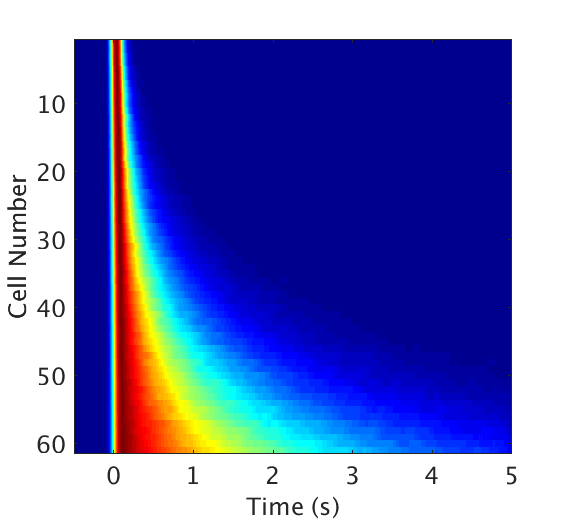
\includegraphics[width=.99\linewidth]{figs/HeatmapExpDecayV2.png}
			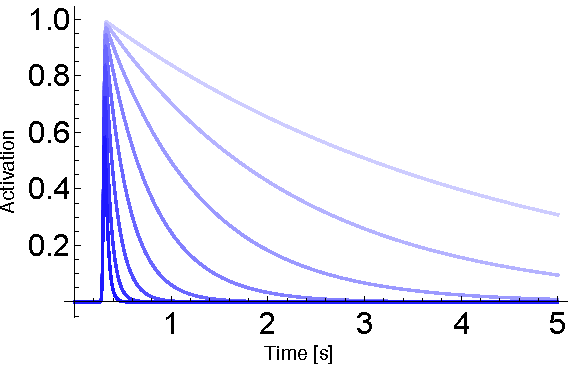
\includegraphics[width=.99\linewidth]{figs/ExpDecParams.pdf}
		\end{center}
	\end{minipage}
	\begin{minipage}{.25\linewidth}
		\textbf{b}
		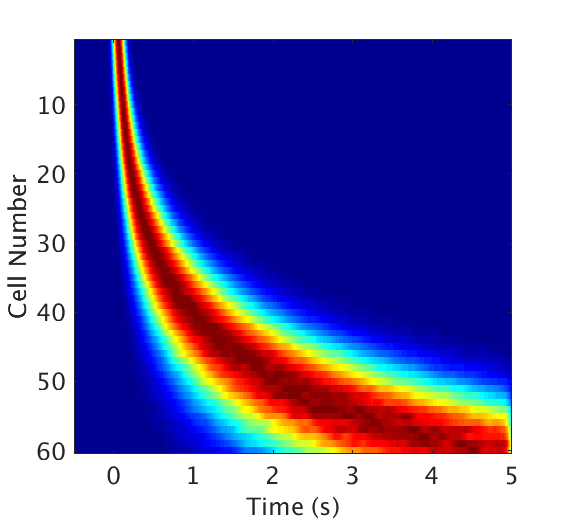
\includegraphics[width=.99\linewidth]{figs/HeatmapTimeCellsV2.png}
		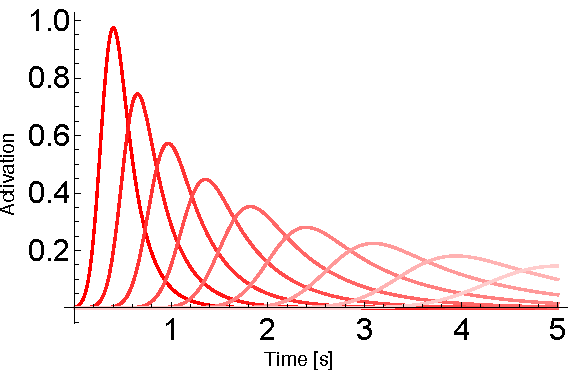
\includegraphics[width=.99\linewidth]{figs/TimeCellParams.pdf}
	\end{minipage}
	\begin{minipage}{0.5\linewidth}
		\textbf{c}
		\begin{center}
			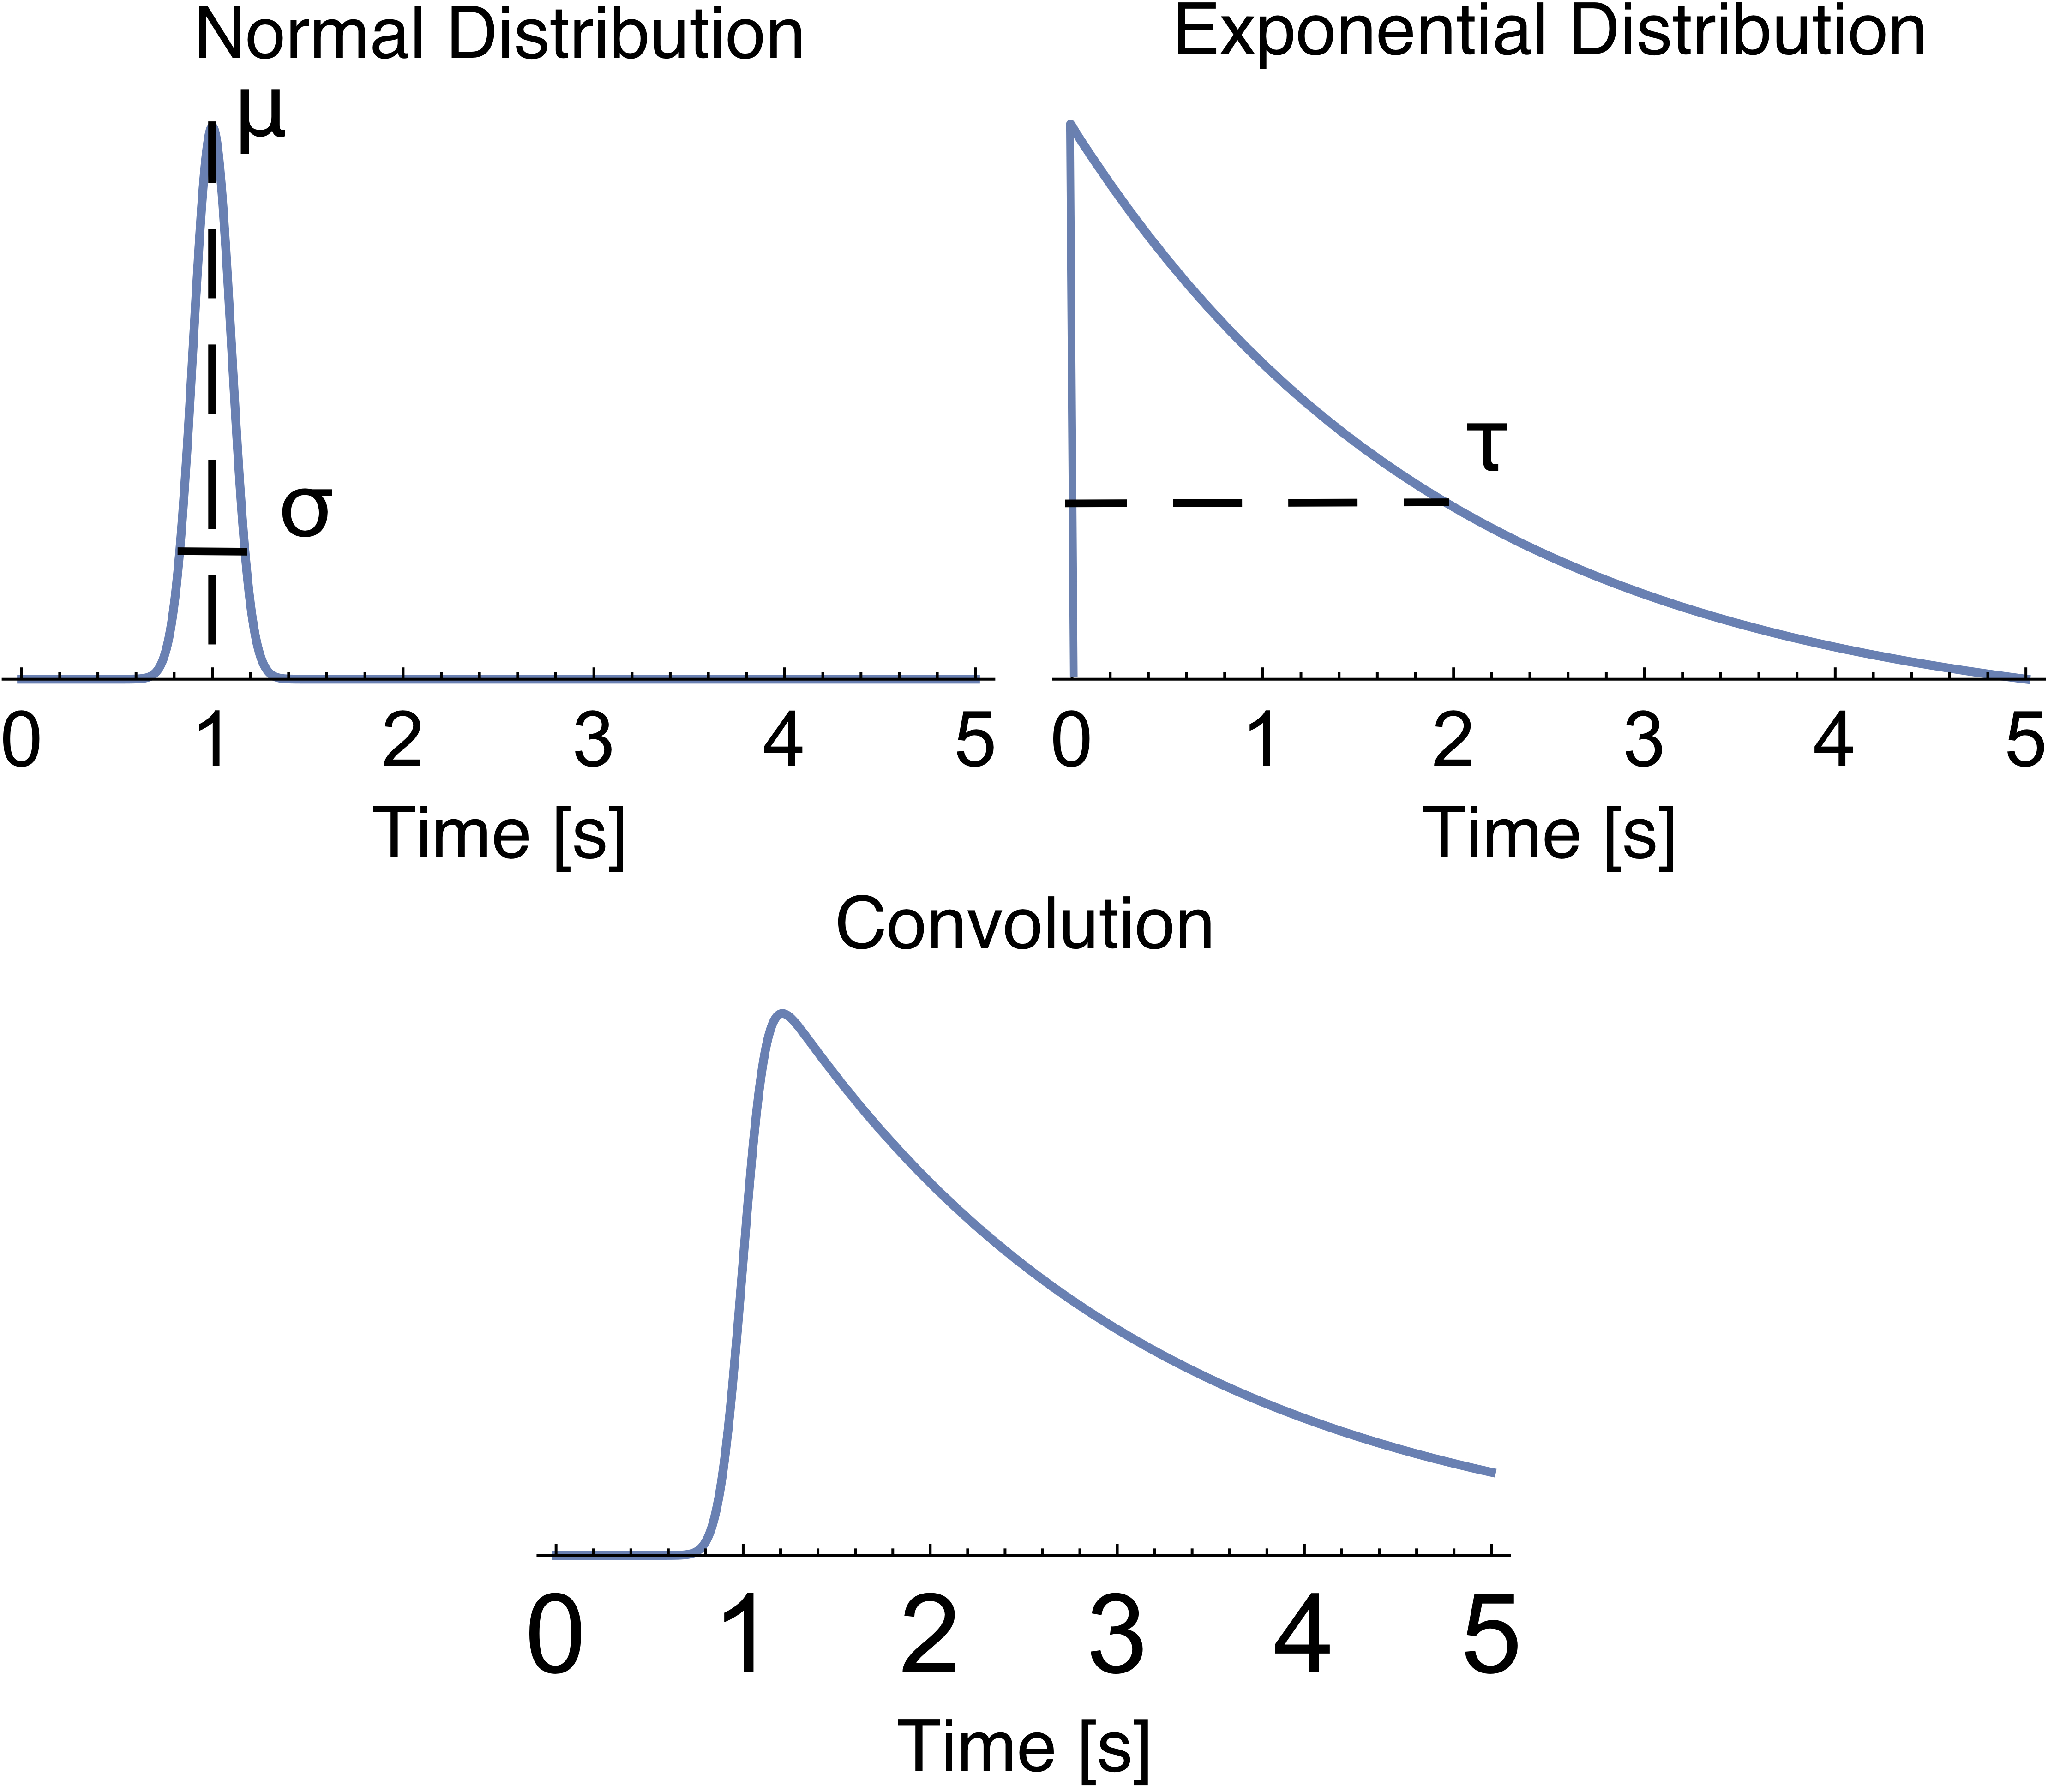
\includegraphics[width=.98\linewidth]{figs/alldists.jpg}
		\end{center}
	\end{minipage}
	\begin{minipage}{0.5\linewidth}
		\textbf{d}
		\begin{flushleft}
			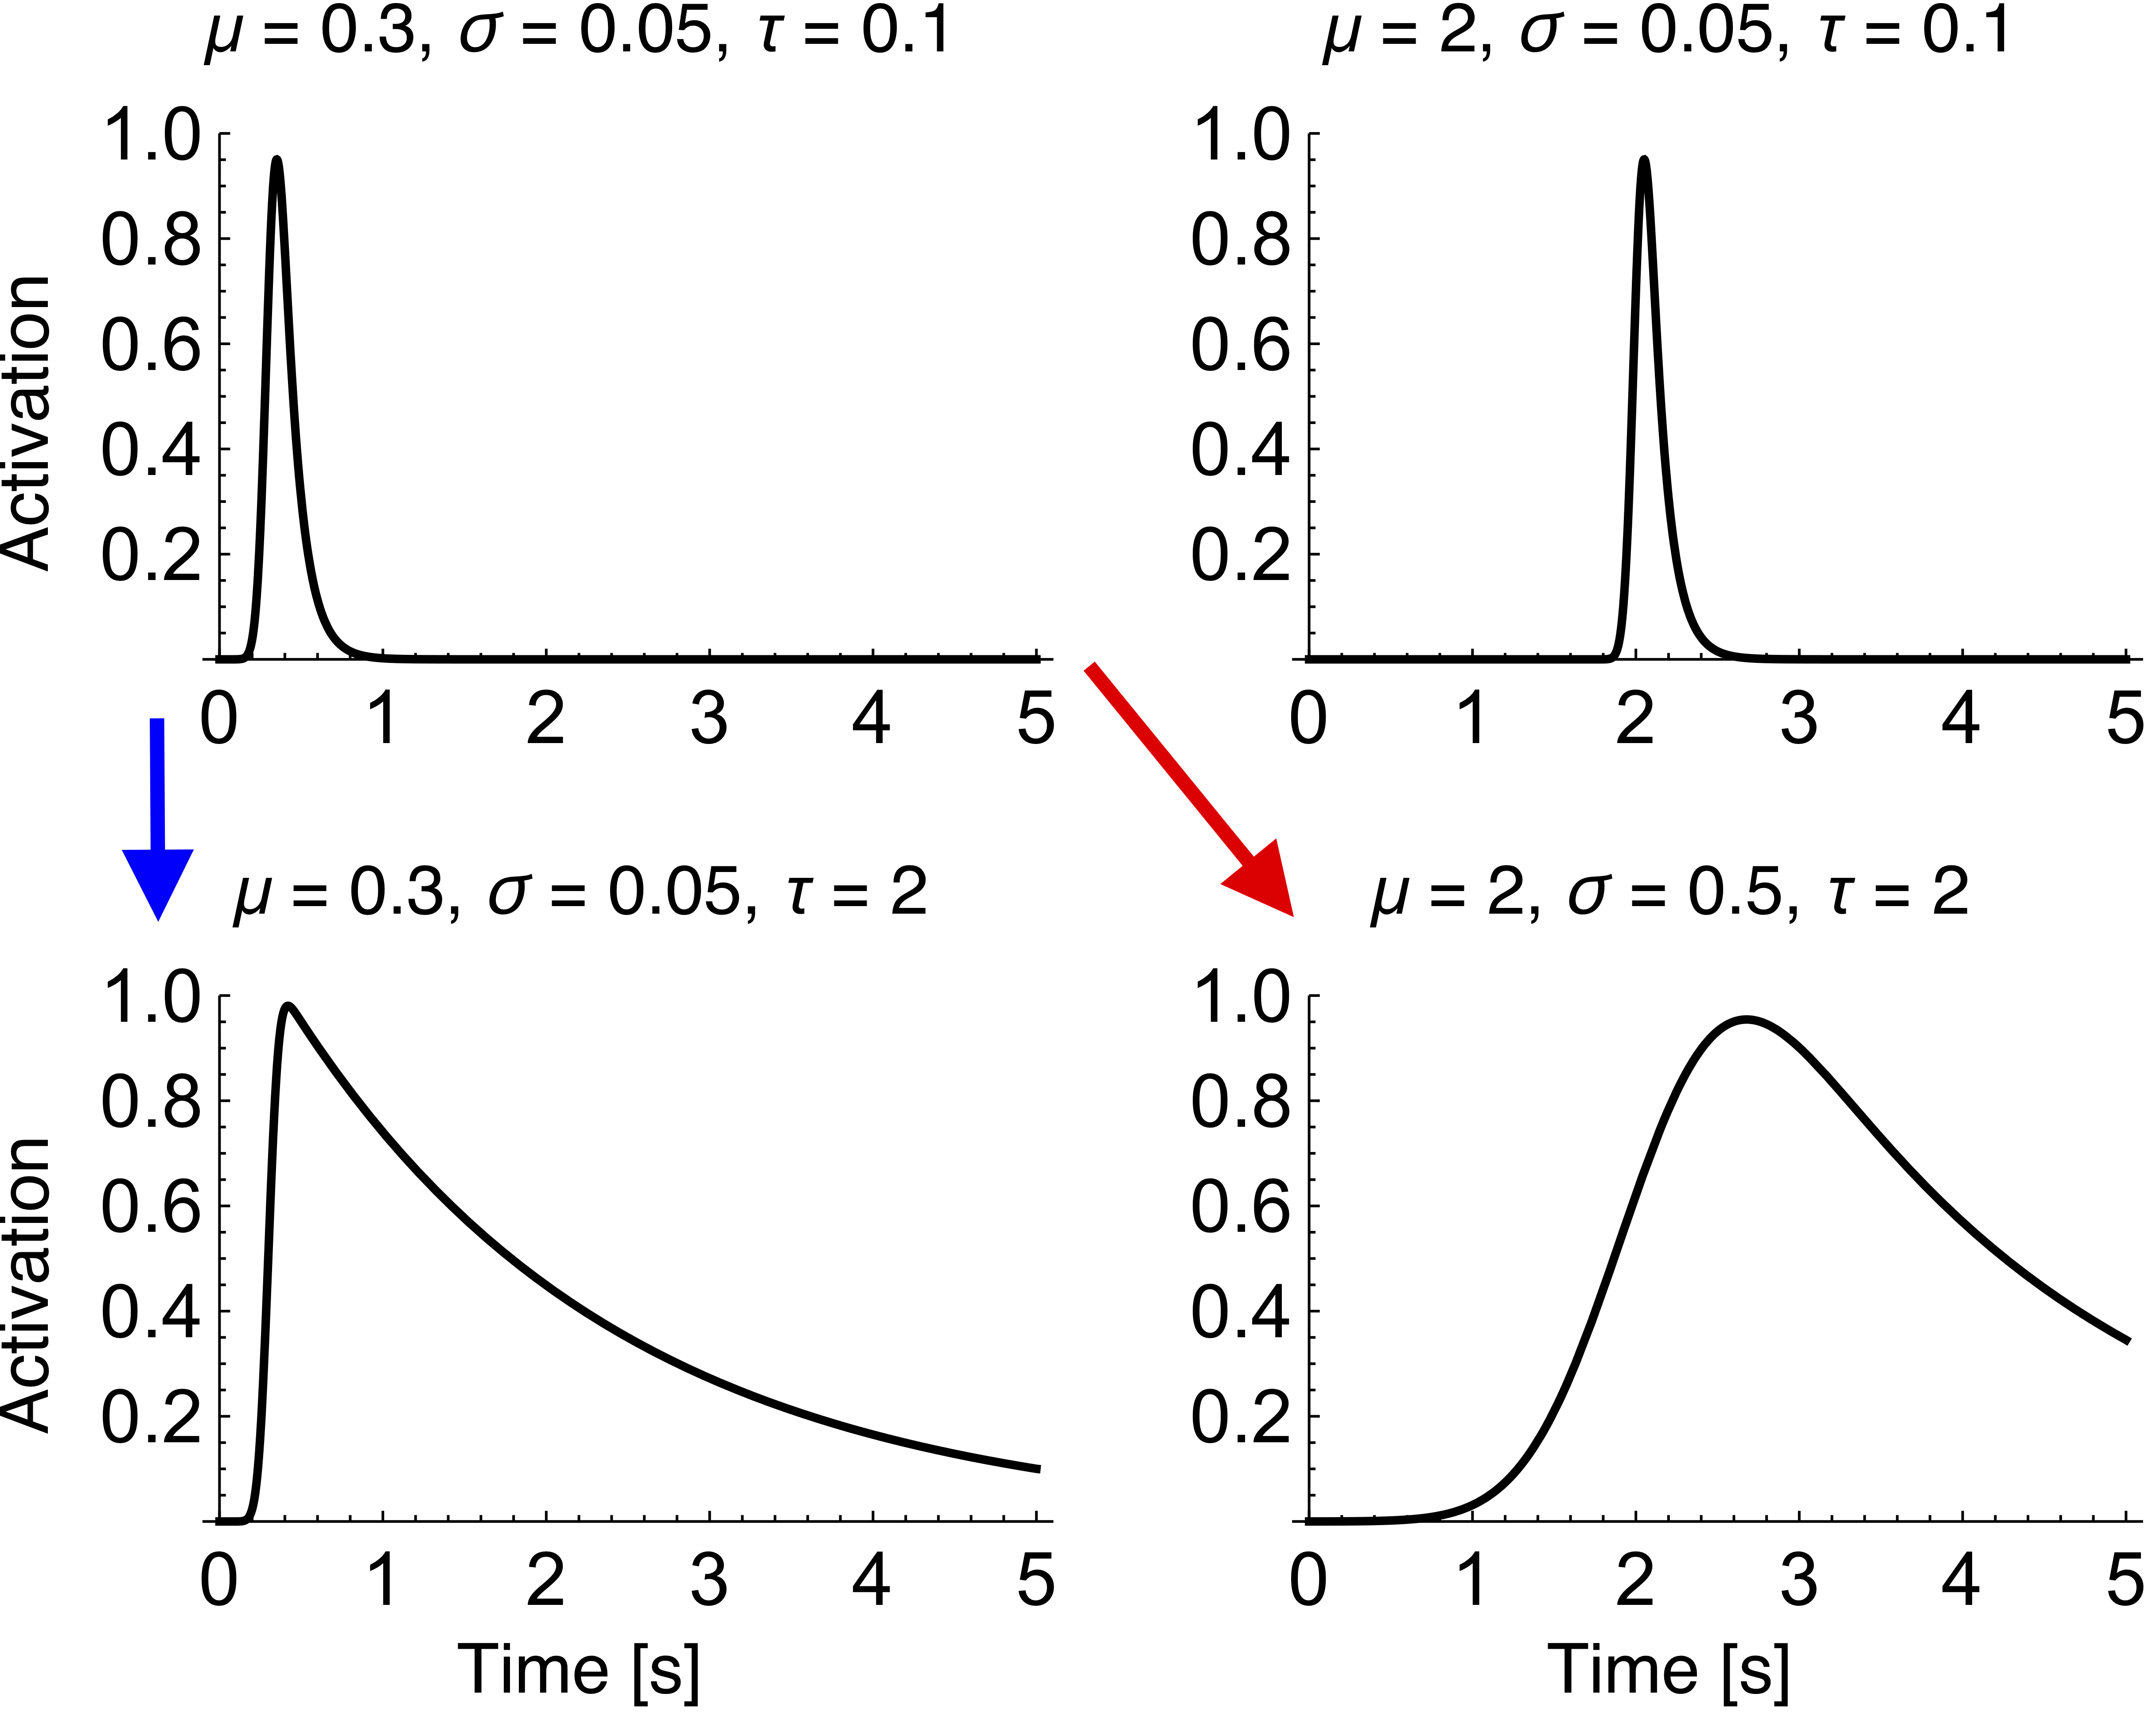
\includegraphics[width=.98\linewidth]{figs/allexamples2.jpg}
		\end{flushleft}
	\end{minipage}
	\begin{minipage}{.5\linewidth}
		\textbf{e}
		\begin{flushleft}
		%\includegraphics[width=.49\linewidth]{figs/BothParams.pdf}
		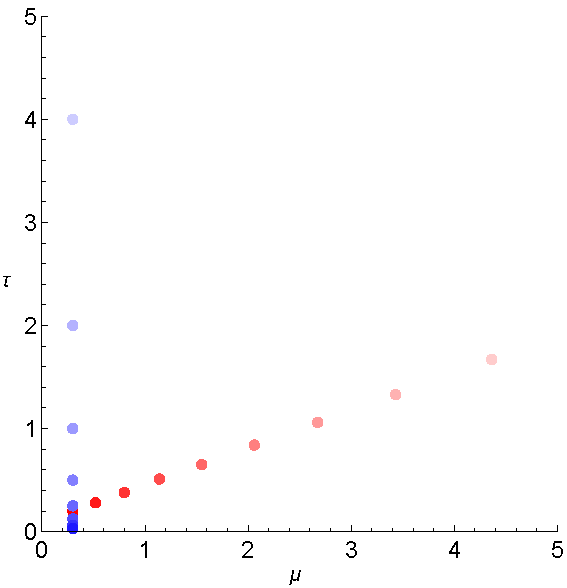
\includegraphics[width = .98\linewidth]{figs/Mu_Tau.pdf}
		\end{flushleft}
	\end{minipage}
	\caption{
		\label{fig:SMTschematic} 
		\textbf{Two Ways of Encoding the Recent Past.} 
		\textbf{a}, Top, heatplot of ideal exponentially decaying cells.
		Bottom, tuning curves of exponentially decaying cells. Cells all peak
		at the beginning of a time interval, but decay at different rates, as
		indicated by line shade. 
		\textbf{b}, Top, heatplot of ideal sequentially activated time cells.
		Bottom, tuning curves of time cells.  Cell peaks span a given time
		interval, as indicated by line shade, and widen their receptive field
		the later in a time interval they peak. 
		\textbf{c}, The convolution model (bottom) is formed by the
		combination of a Gaussian distribution, with parameters $\mu$ and
		$\sigma$ and an exponential distribution, with parameter $\tau$ (top).
		\textbf{d}, In the convolution model, an increase in $\mu$ shifts the
		distribution to the right, an increase in $\sigma$ widens the entire
		distribution, and an increase in $\tau$ lengthens its decay rate. The
		blue and red arrows correspond to the parameter changes expected of
		exponentially decaying and sequentially activated time cells
		respectively. 
		\textbf{e}, Values of $\mu$ and $\tau$ of the cells plotted in the
		bottom of \textbf{a} and \textbf{b}. A population of exponentially
		decaying cells all have small $\mu$ values but show a variety of
		$\tau$ values. Time cells show values of $\mu$ that span a time span,
		with $\tau$ values that increase with $\mu$.
	}
\end{figure}

\subsubsection{Empirical results for model parameters}
Results for $\mu$ and $\tau$ are discussed in detail in the main text.  The values
of $\sigma$ were small and tightly clustered.  



\subsection{Temporal decoding from ideal sequentially-activated time cells and
exponentially-decaying units}

This technique is demonstrated on
simulated exponentially decaying cells and simulated time cells in Figure
\ref{fig:LDA_simulated}.  The decoding error appears to behave similarly for
both ideal time cells and exponentially decaying cells. 

\begin{figure}
\begin{tabular}[t]{l c l c}
\textbf{a} & & \textbf{b}& \\
&
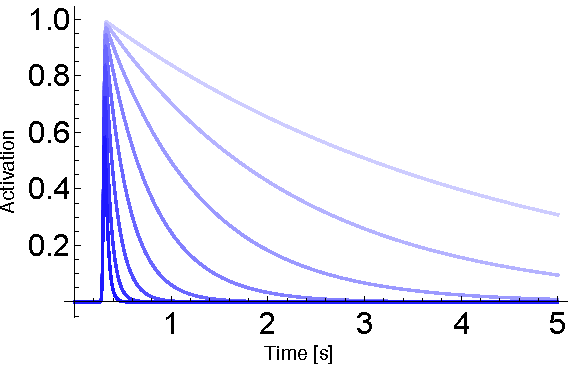
\includegraphics[width=.4\linewidth]{figs/ExpDecParams.pdf}
&
&
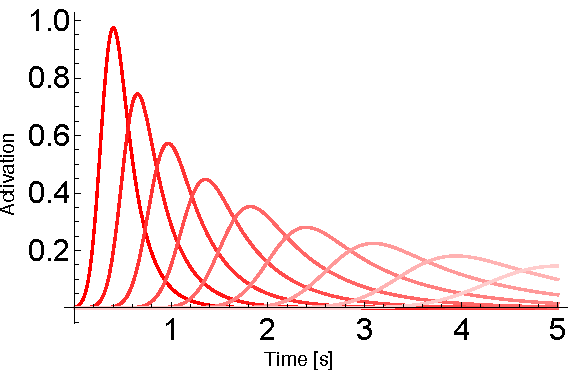
\includegraphics[width=.4\linewidth]{figs/TimeCellParams.pdf}
\\
\textbf{c} & & \textbf{d}& \\
 & 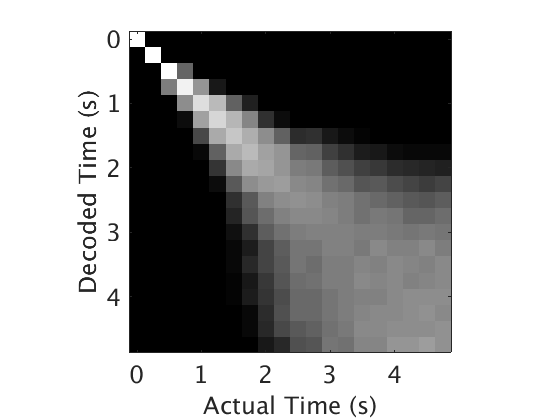
\includegraphics[width=.45\linewidth]{figs/LogPosteriorExpDecay_75noiseV3.png}
& & 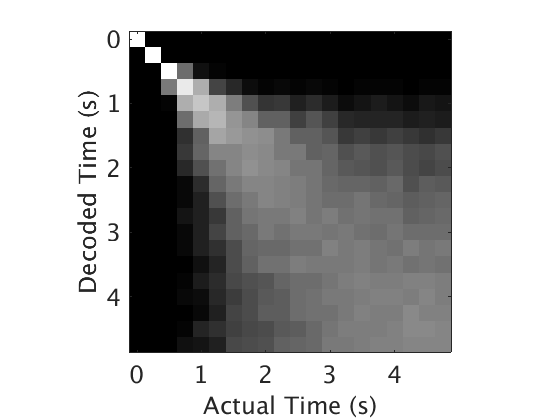
\includegraphics[width=.45\linewidth]{figs/LogPosteriorTimeCells_20noiseV3.png}
\\
\textbf{e} & & \textbf{f}& \\
 & 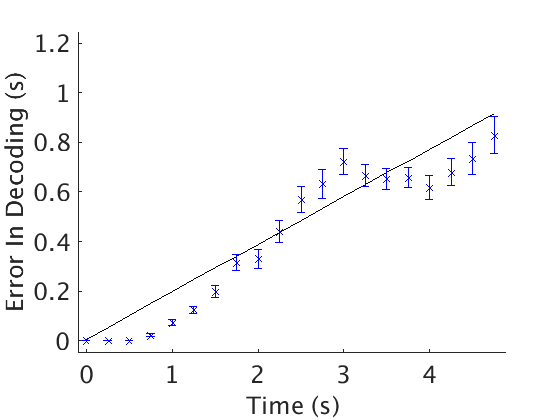
\includegraphics[width=.4\linewidth]{figs/AbsErrorExpDecay_75noiseV3.png} 
 & &
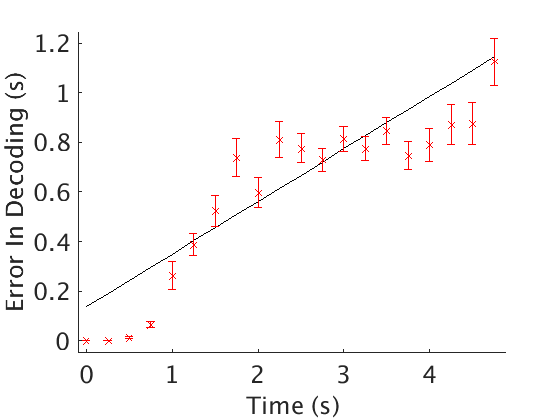
\includegraphics[width=.4\linewidth]{figs/AbsErrorTimeCells_20noiseV3.png}
\end{tabular}
\caption{\textbf{Time can be decoded from both time cells and exponentially
decaying cells with decreasing accuracy as time unfolds.} Simulated noisy
time cells and exponentially decaying cells.  Time is binned in 250ms bins.  A
linear decoder is trained on odd trials and tested on even trials.  \textbf{a}
An illustration of a small collection of exponentially decaying cells.  The
actual simulated data set used 30 cells with time constants ranging from 50 ms
to 10s. \textbf{b} An illustration of a collection of ideal time cells.  The
actual simulated data set used 30 cells with time constants ranging from 50ms
to 10s.  \textbf{c}, \textbf{d} Log of the posterior probabilities.  The
posterior probabilities of the classify function are averaged across trials
for each time bin.  Perfect decoding would look like a white diagonal.  In
order to show the distinction between small values, the log of the averaged
posterior probabilities plus a small threshold is shown here.  The posterior
distribution of the classifier shows an increasing spread in the model's
estimation of decoded time. \textbf{e}, \textbf{f} Averaged absolute value of
decoding error.  The decoding error goes up with time, as shown by the fitted
regression line (black line). }
\label{fig:LDA_simulated} 
\end{figure}

\begin{figure}
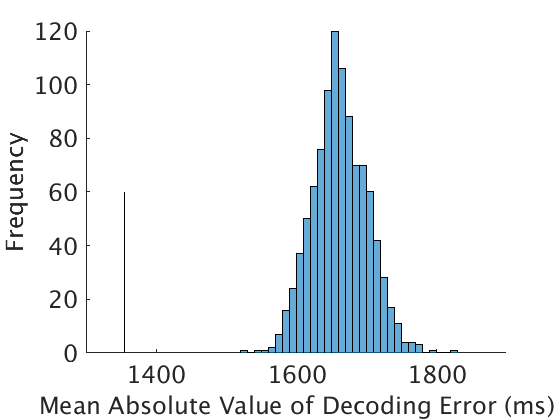
\includegraphics[width=.7\linewidth]{figs/Permutest.png}
\caption{\textbf{Data with permuted labels contains less information than the original data.}. 
The histogram shows the distribution of mean absolute value of decoding error for the permuted data.  
The mean absolute value of decoding error for the original data is marked with the line.  
The original data's decoding error is clearly different from that of the permuted data.  This indicates the decoding is significantly better than chance.}
\label{fig:permutest}
\end{figure}


 %if we control for the number of cells, other cells are only significant up to 750 ms for permutation test and only significant up to 500ms for chi2squared GoF




\begin{figure}
\begin{tabular}{l l}
\textbf{a}
&\textbf{b}\\
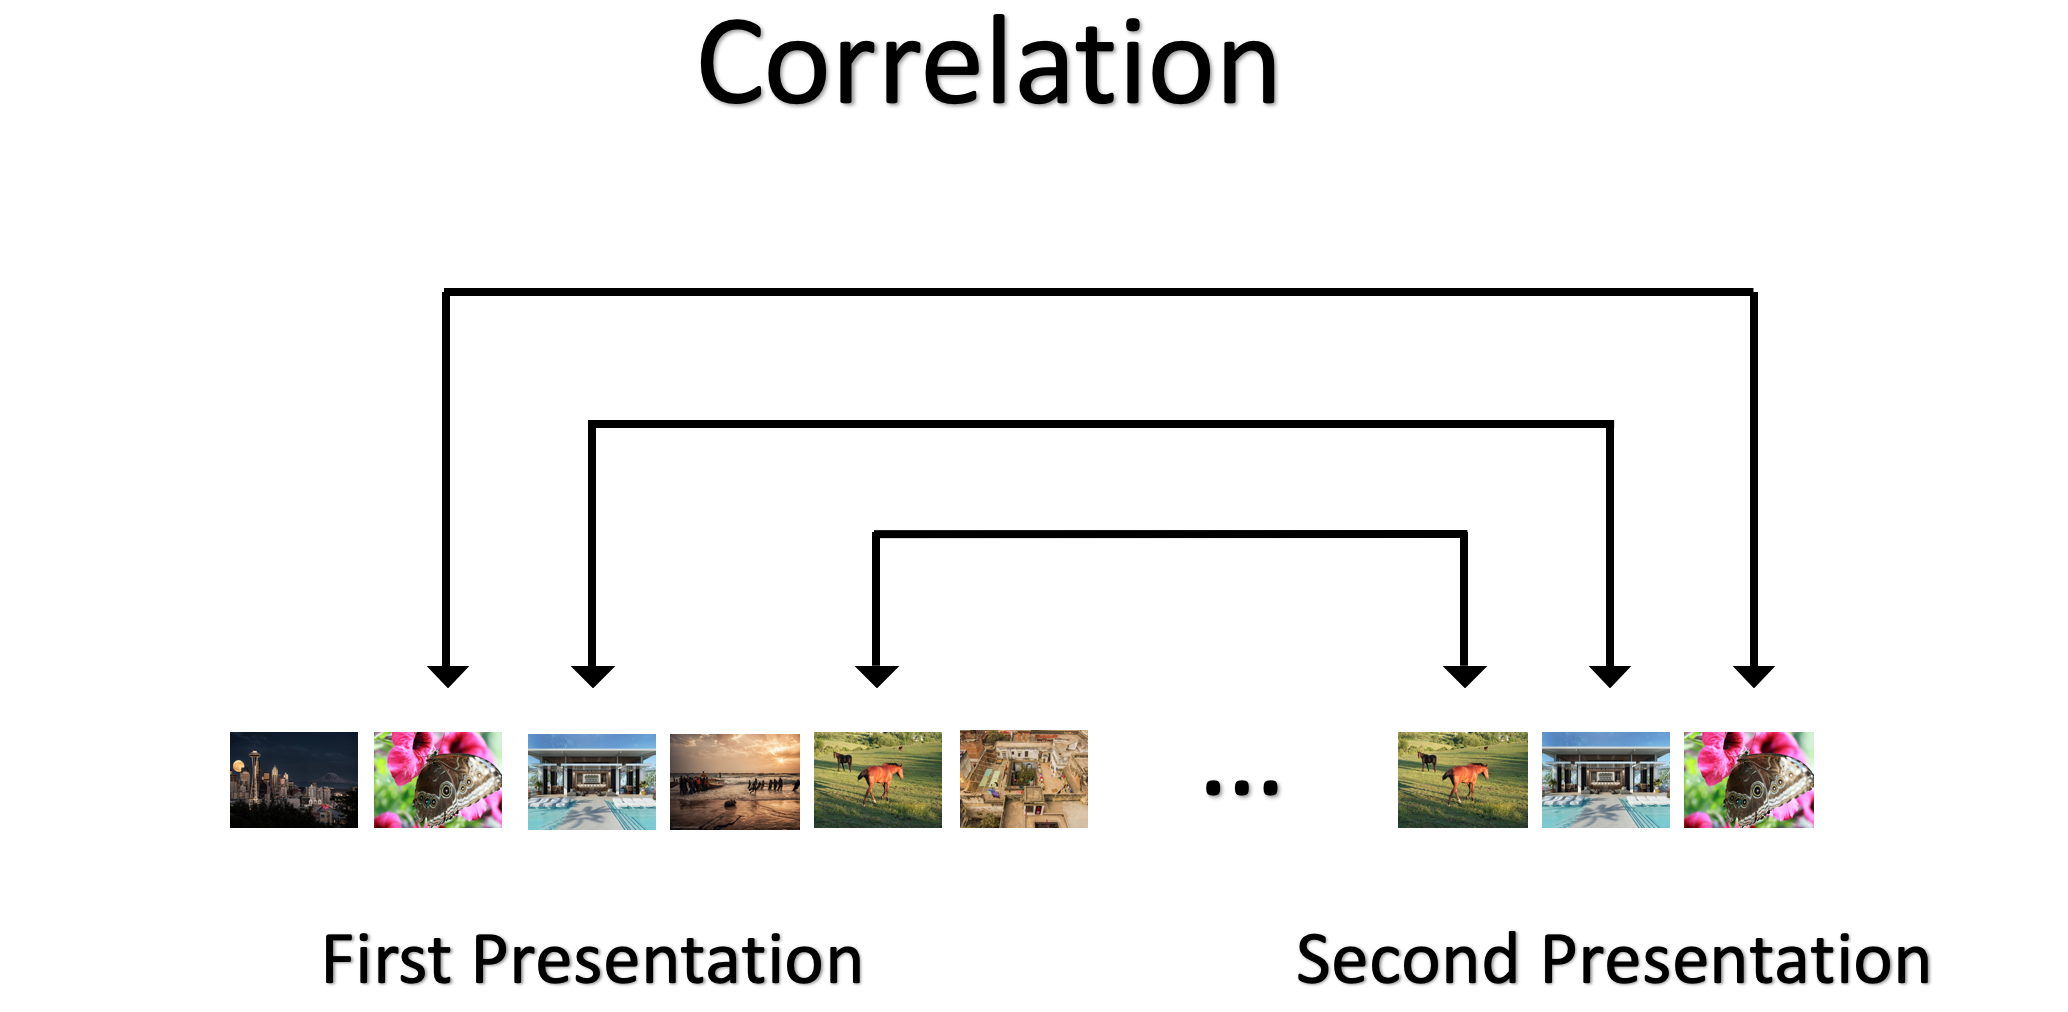
\includegraphics[width =.48\textwidth]{figs/CorrS.png}
&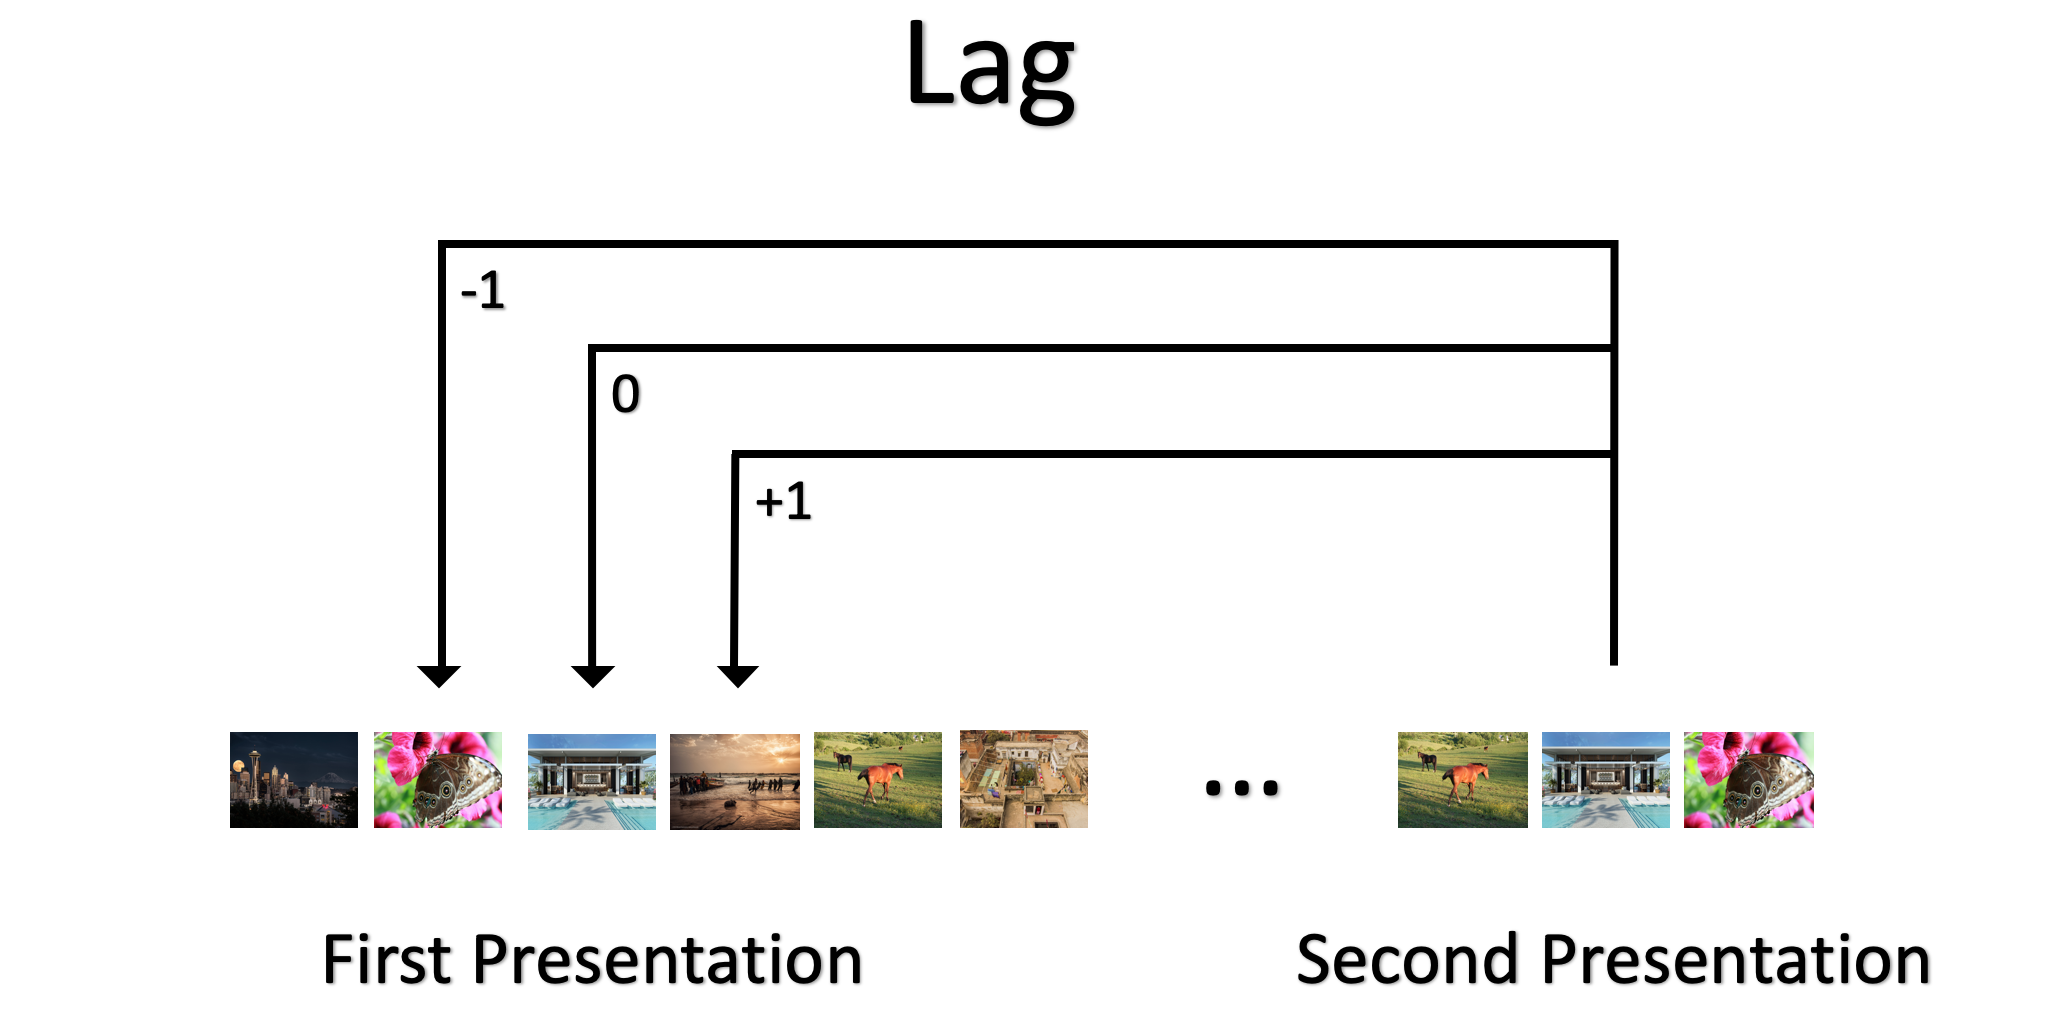
\includegraphics[width = .48\textwidth]{figs/JBITS.png}\\
\textbf{c}
&\textbf{d}\\
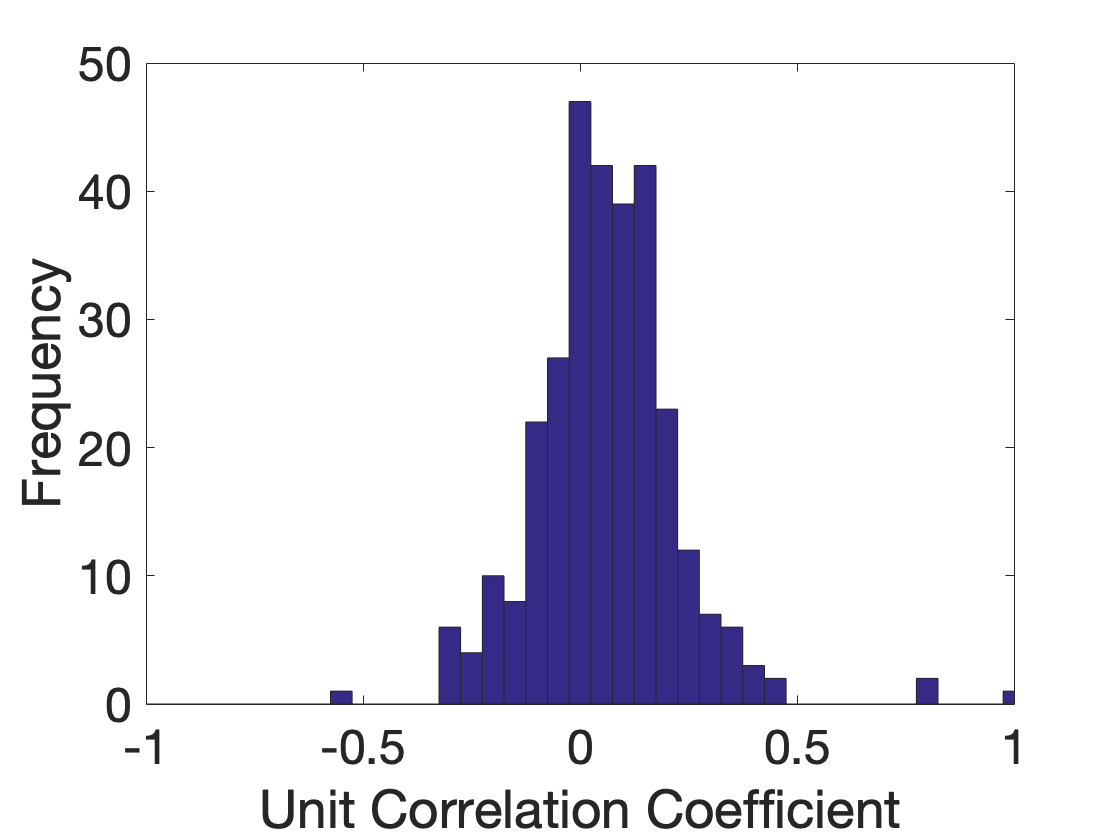
\includegraphics[width = .5\textwidth]{figs/CorrDist.png}
&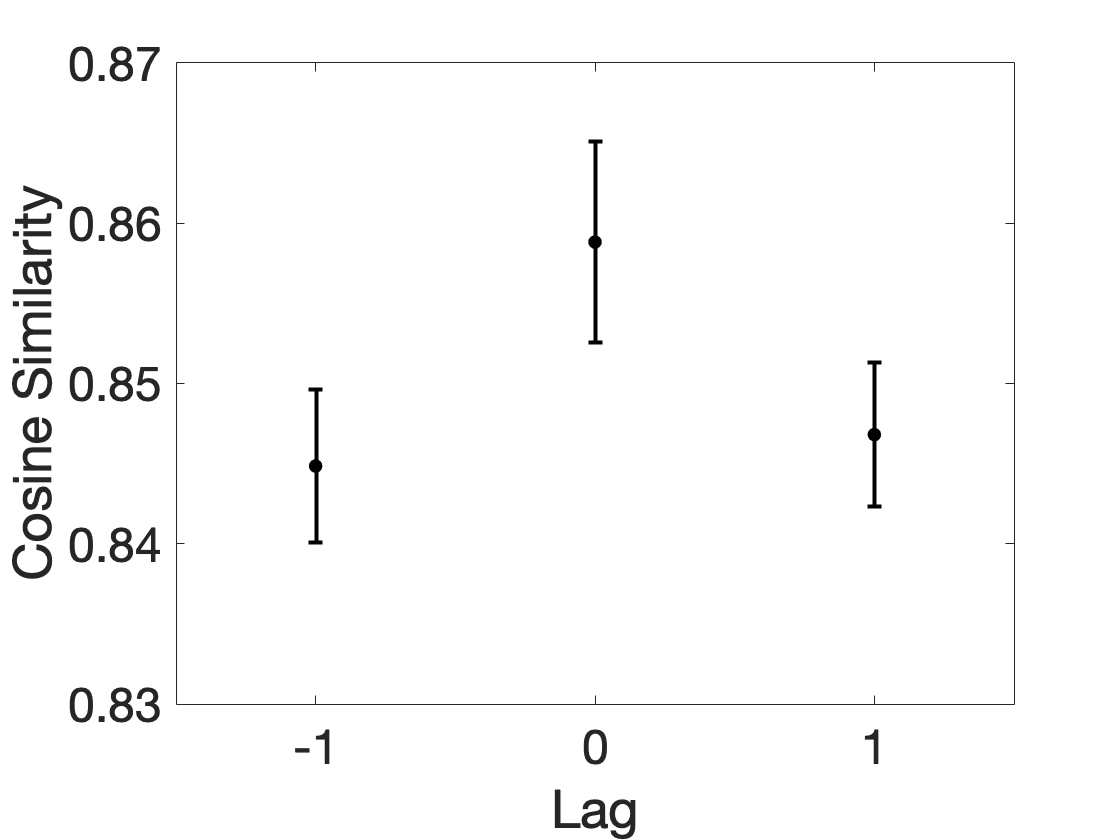
\includegraphics[width = .5\textwidth]{figs/JBIT2.png}
\end{tabular}
\caption{ \textbf{The Entorhinal Ensemble Carries Information About Stimulus Identity.}
\textbf{a}, At the unit level, we measured how correlated spiking activity was in response to the 
same image, as measured by Kendall's $\tau$.
\textbf{b}, In lag analyses the population of cells during the second
presentation of an image is compared to the population of cells during the
first presentation of all images. \textbf{c}, Across the population, unit spiking activity in
response to image repetition was positively correlated. \textbf{d}, There is a significant spike in image
similarity at lag zero (image repetition) compared to lag +1 and lag -1 (adjacent images).} 
\label{fig:StimInfo} 
\end{figure}

\begin{figure}

\begin{tabular}{l l l}
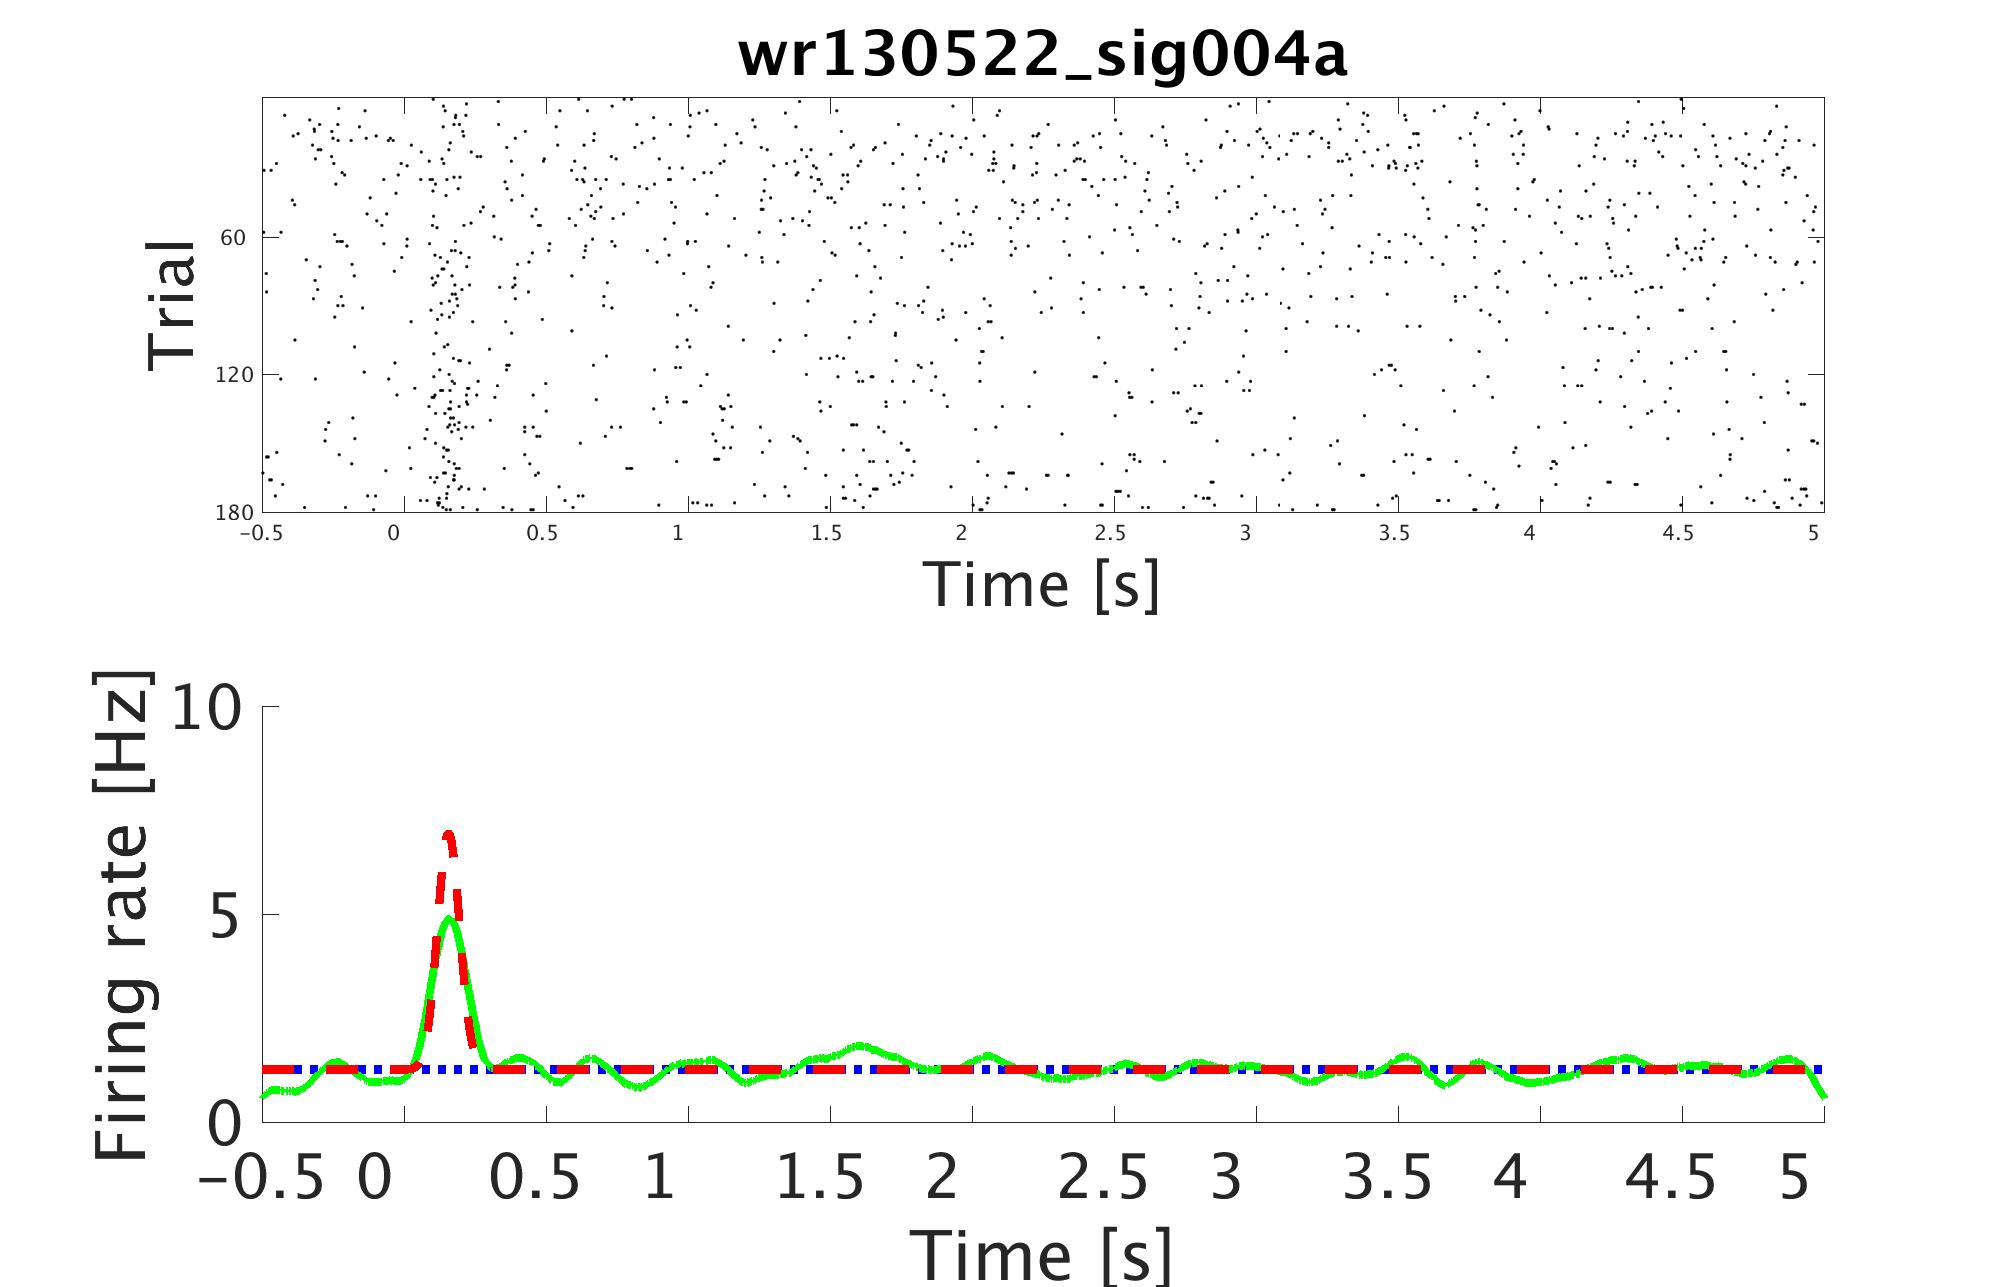
\includegraphics[width =.33\textwidth]{Supplemental_Cells/allcell_138_v_11.jpeg} %0.01
&
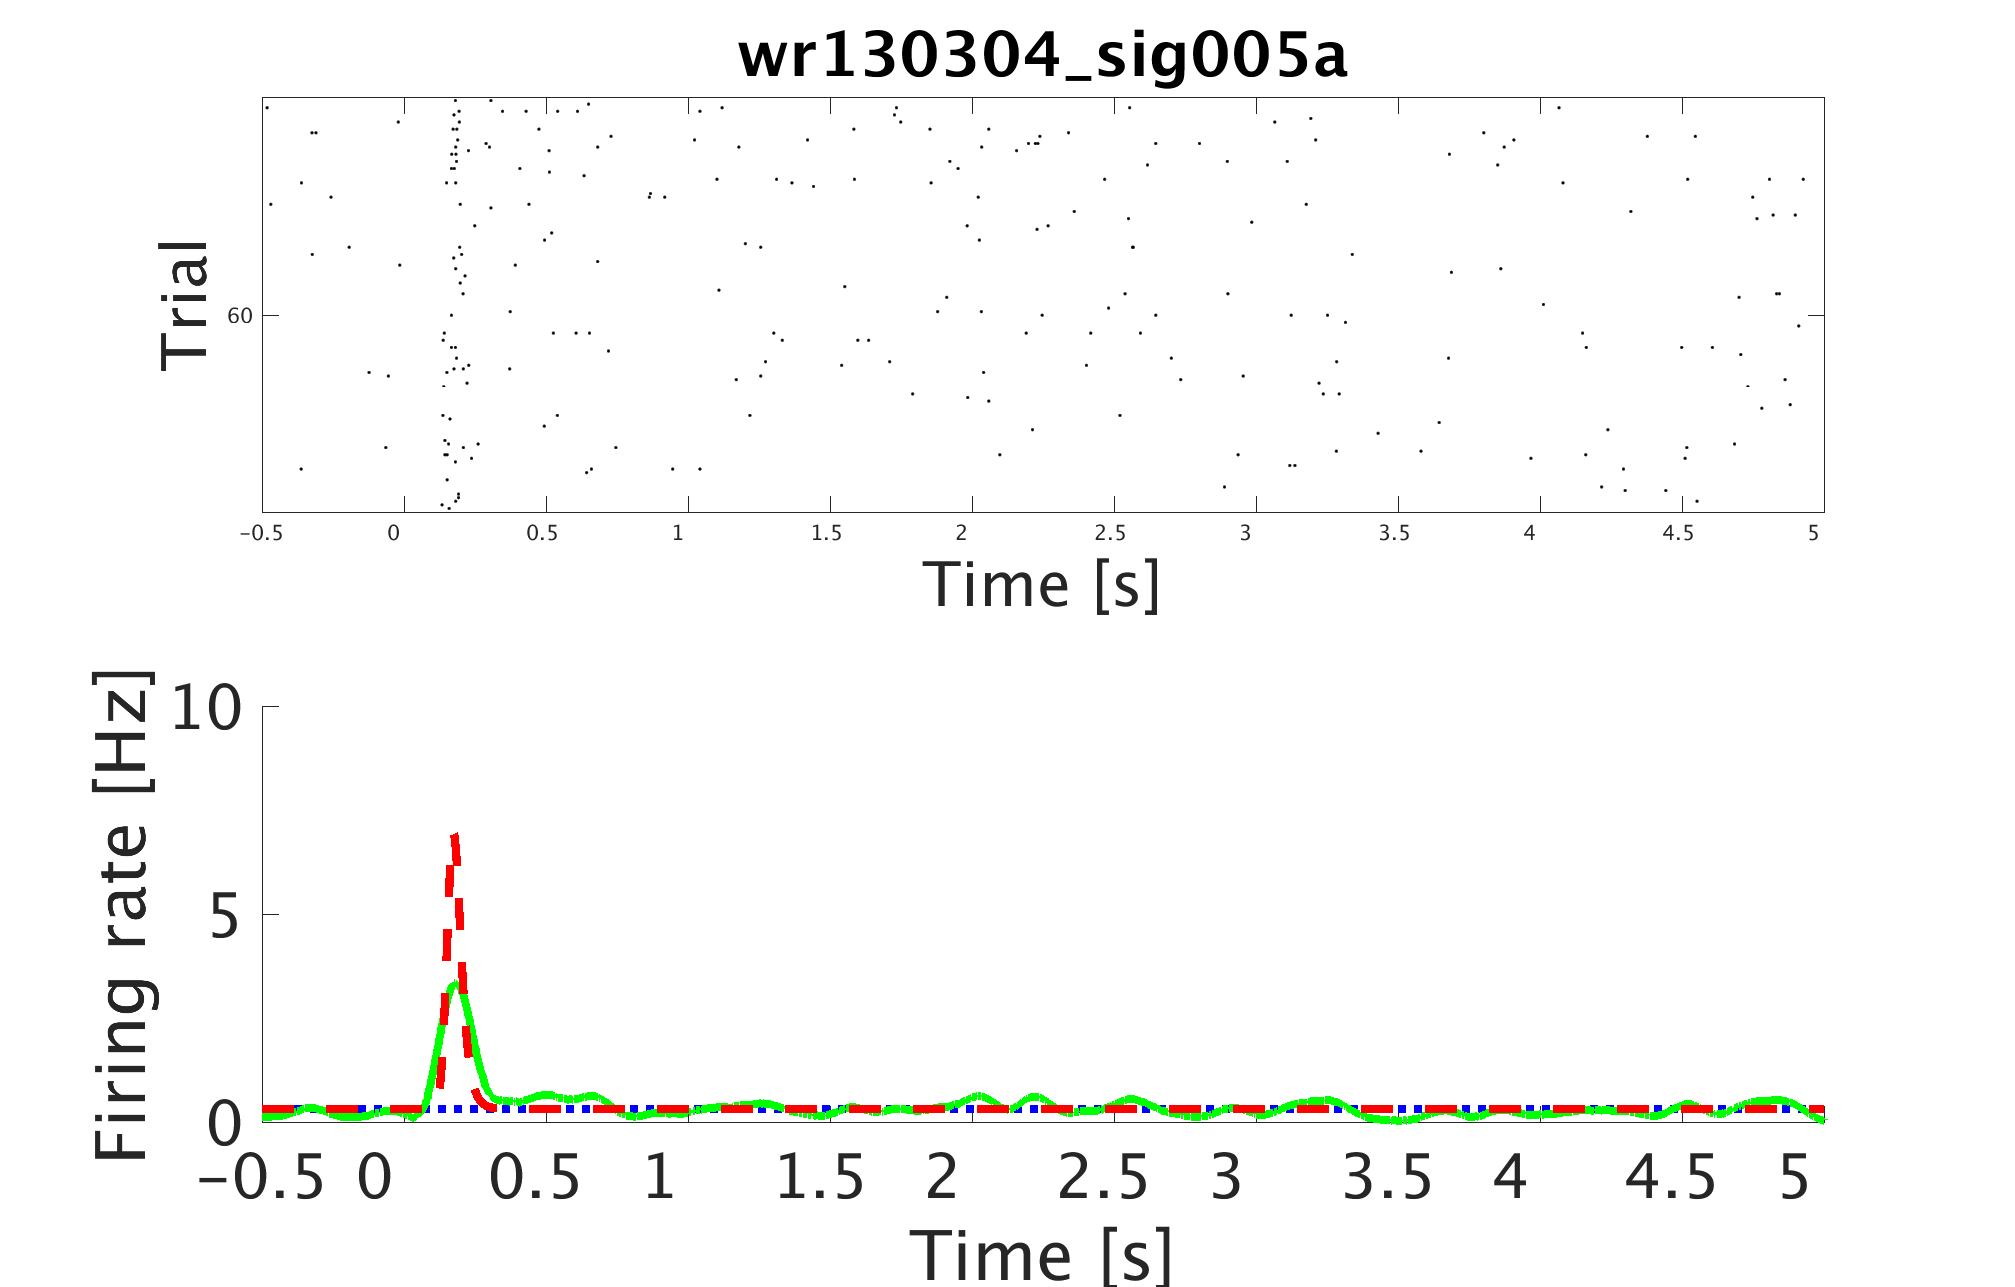
\includegraphics[width =.33\textwidth]{Supplemental_Cells/allcell_92_v_11.jpeg} %.02
&
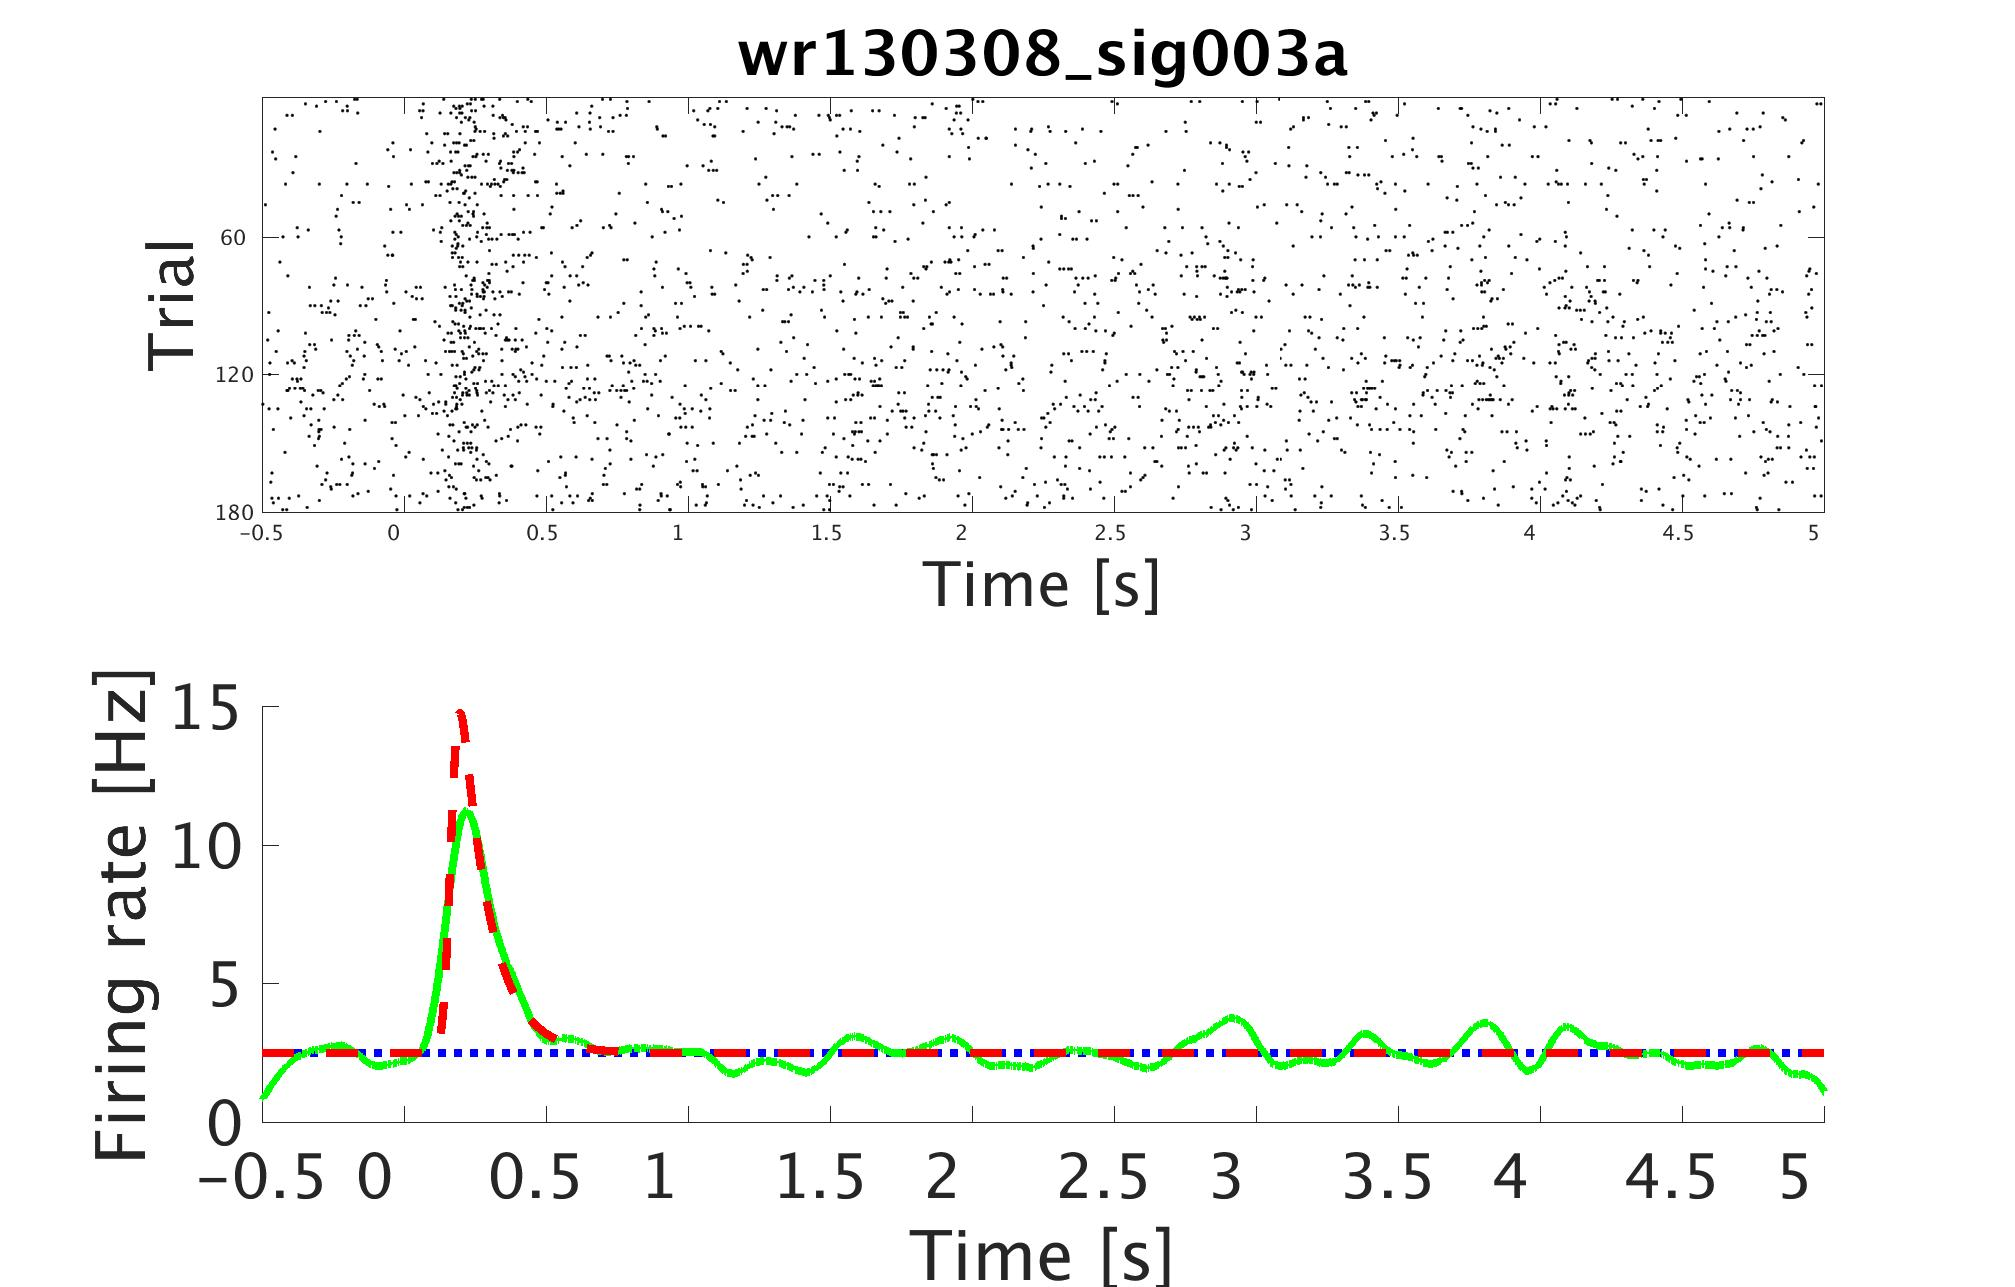
\includegraphics[width =.33\textwidth]{Supplemental_Cells/allcell_101_v_11.jpeg}\\%.10


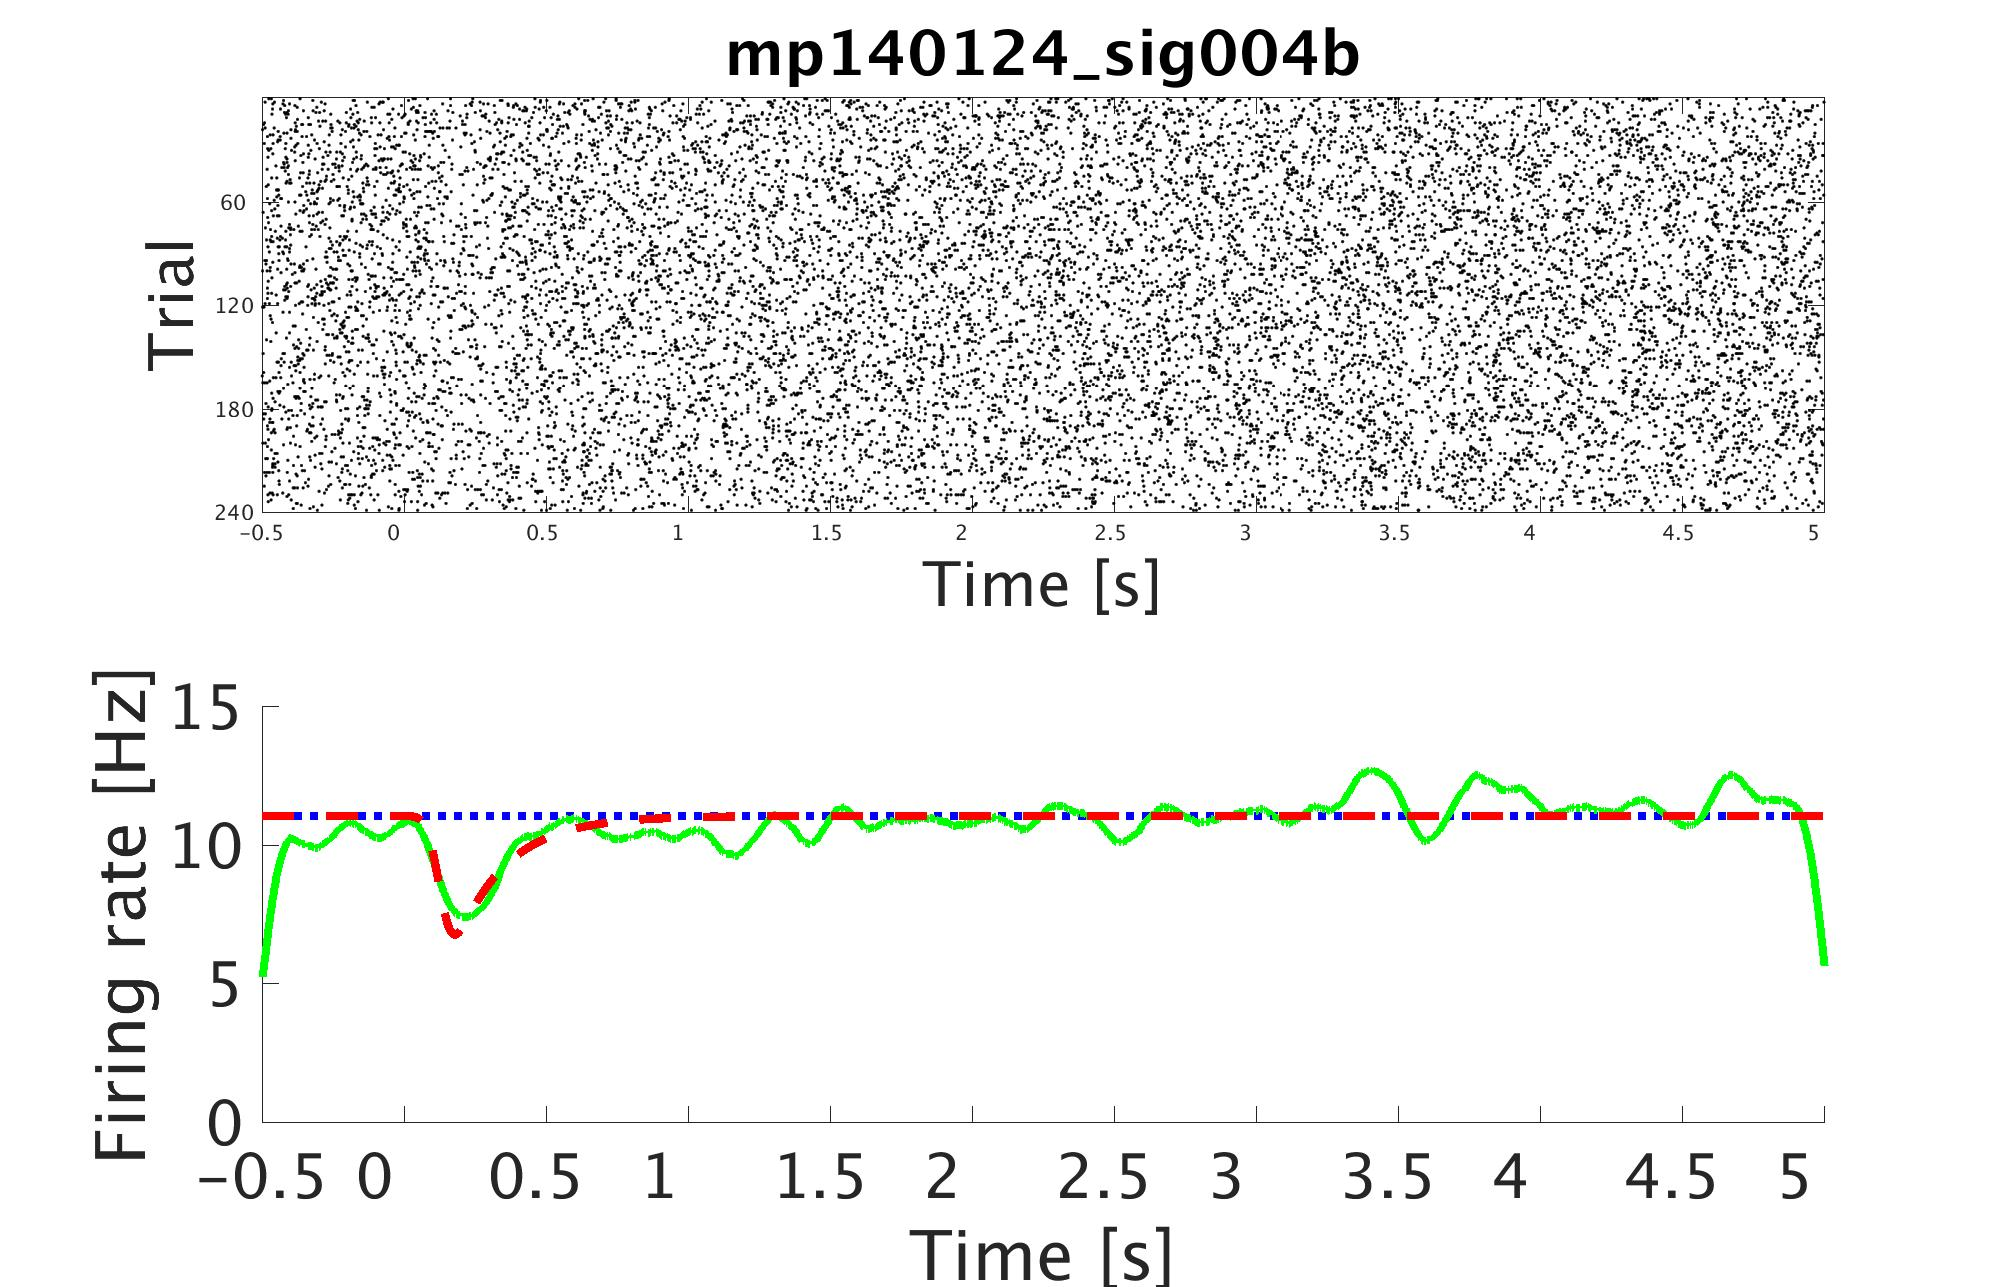
\includegraphics[width =.33\textwidth]{Supplemental_Cells/allcell_292_v_11.jpeg}%.18
&
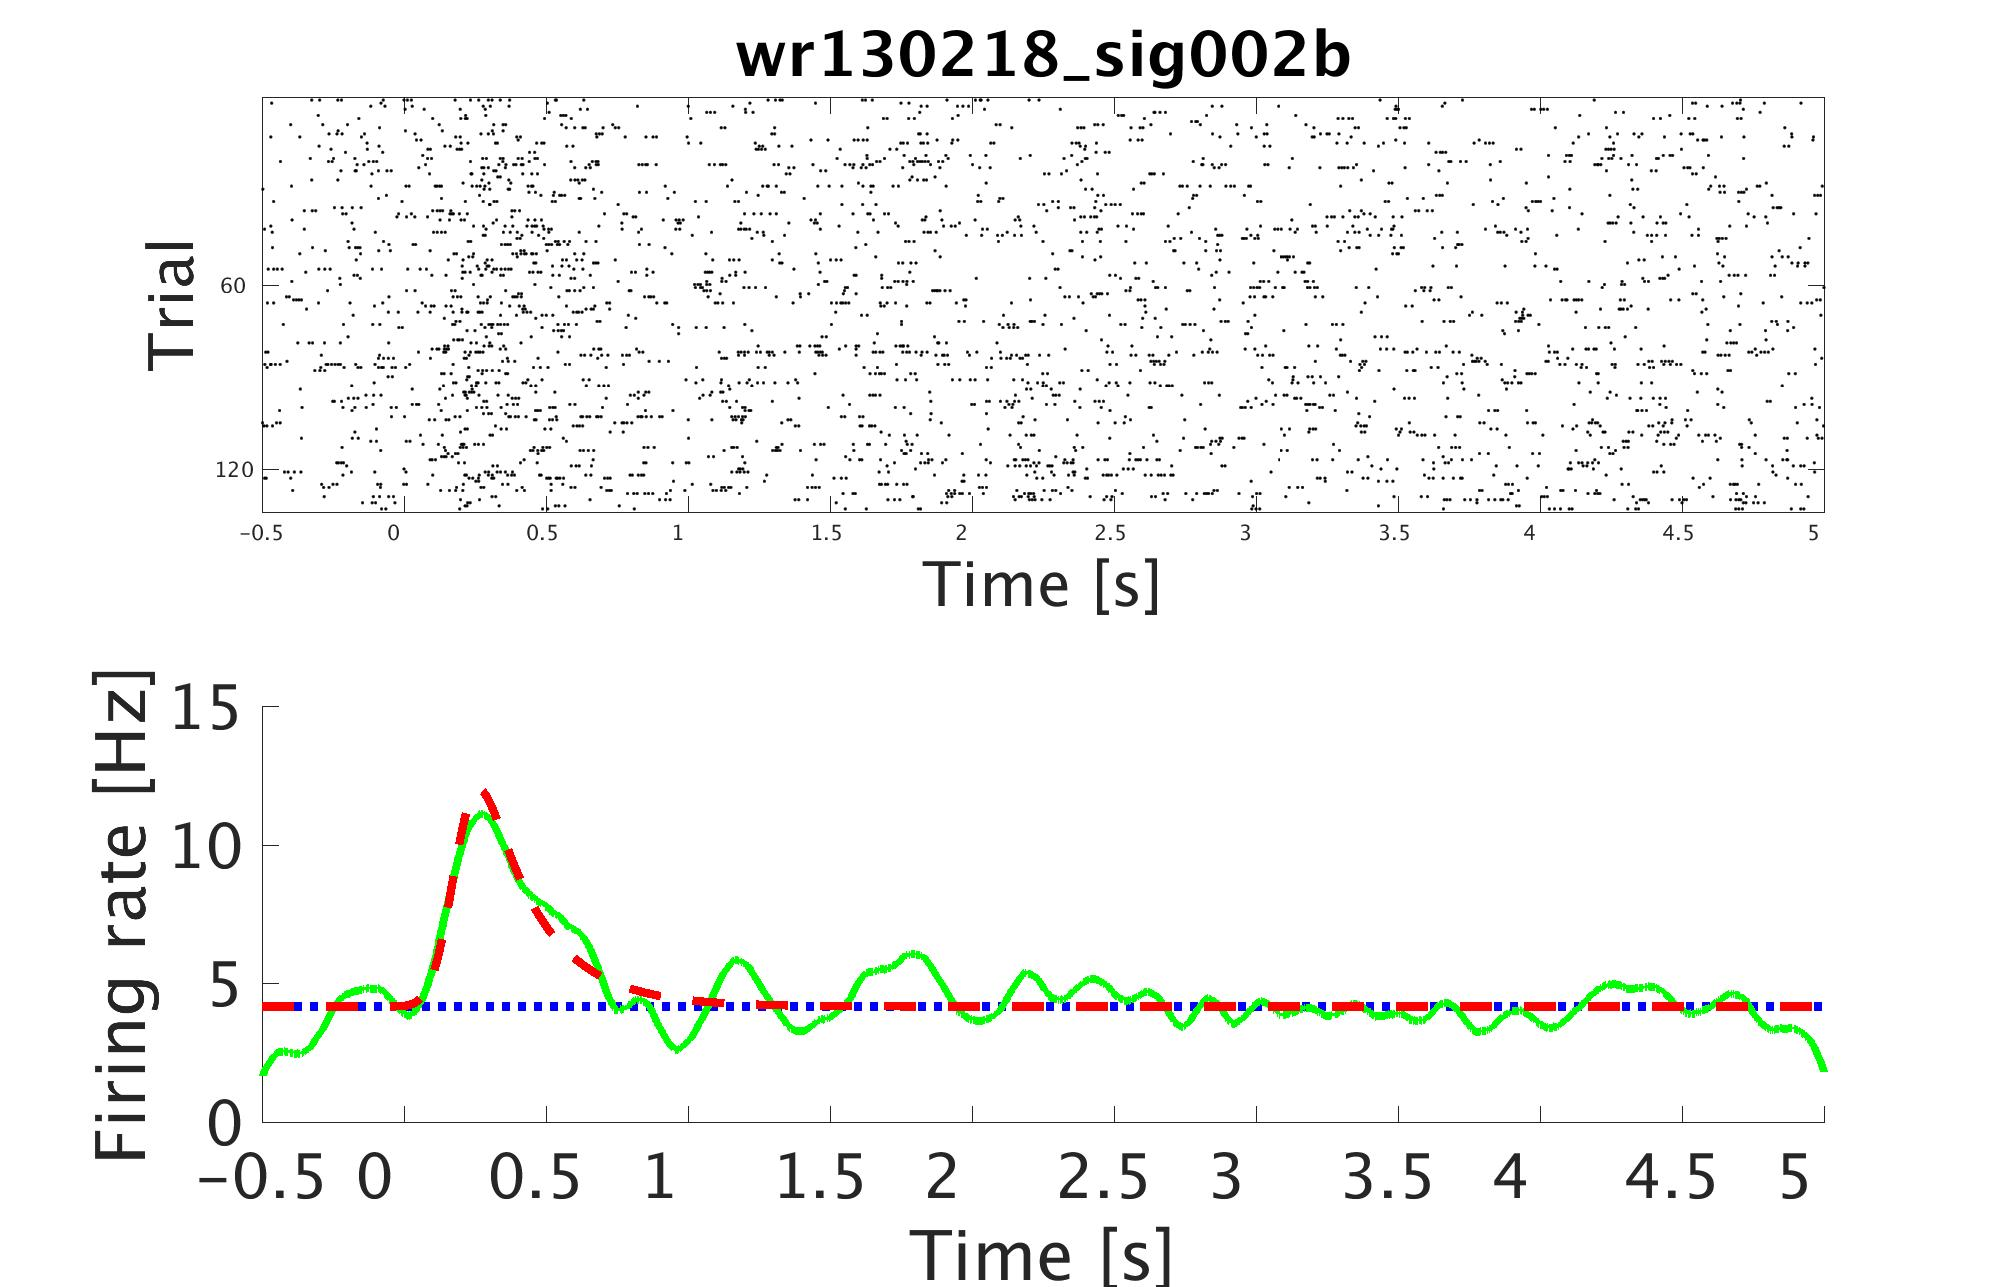
\includegraphics[width =.33\textwidth]{Supplemental_Cells/allcell_35_v_11.jpeg}%.20
&
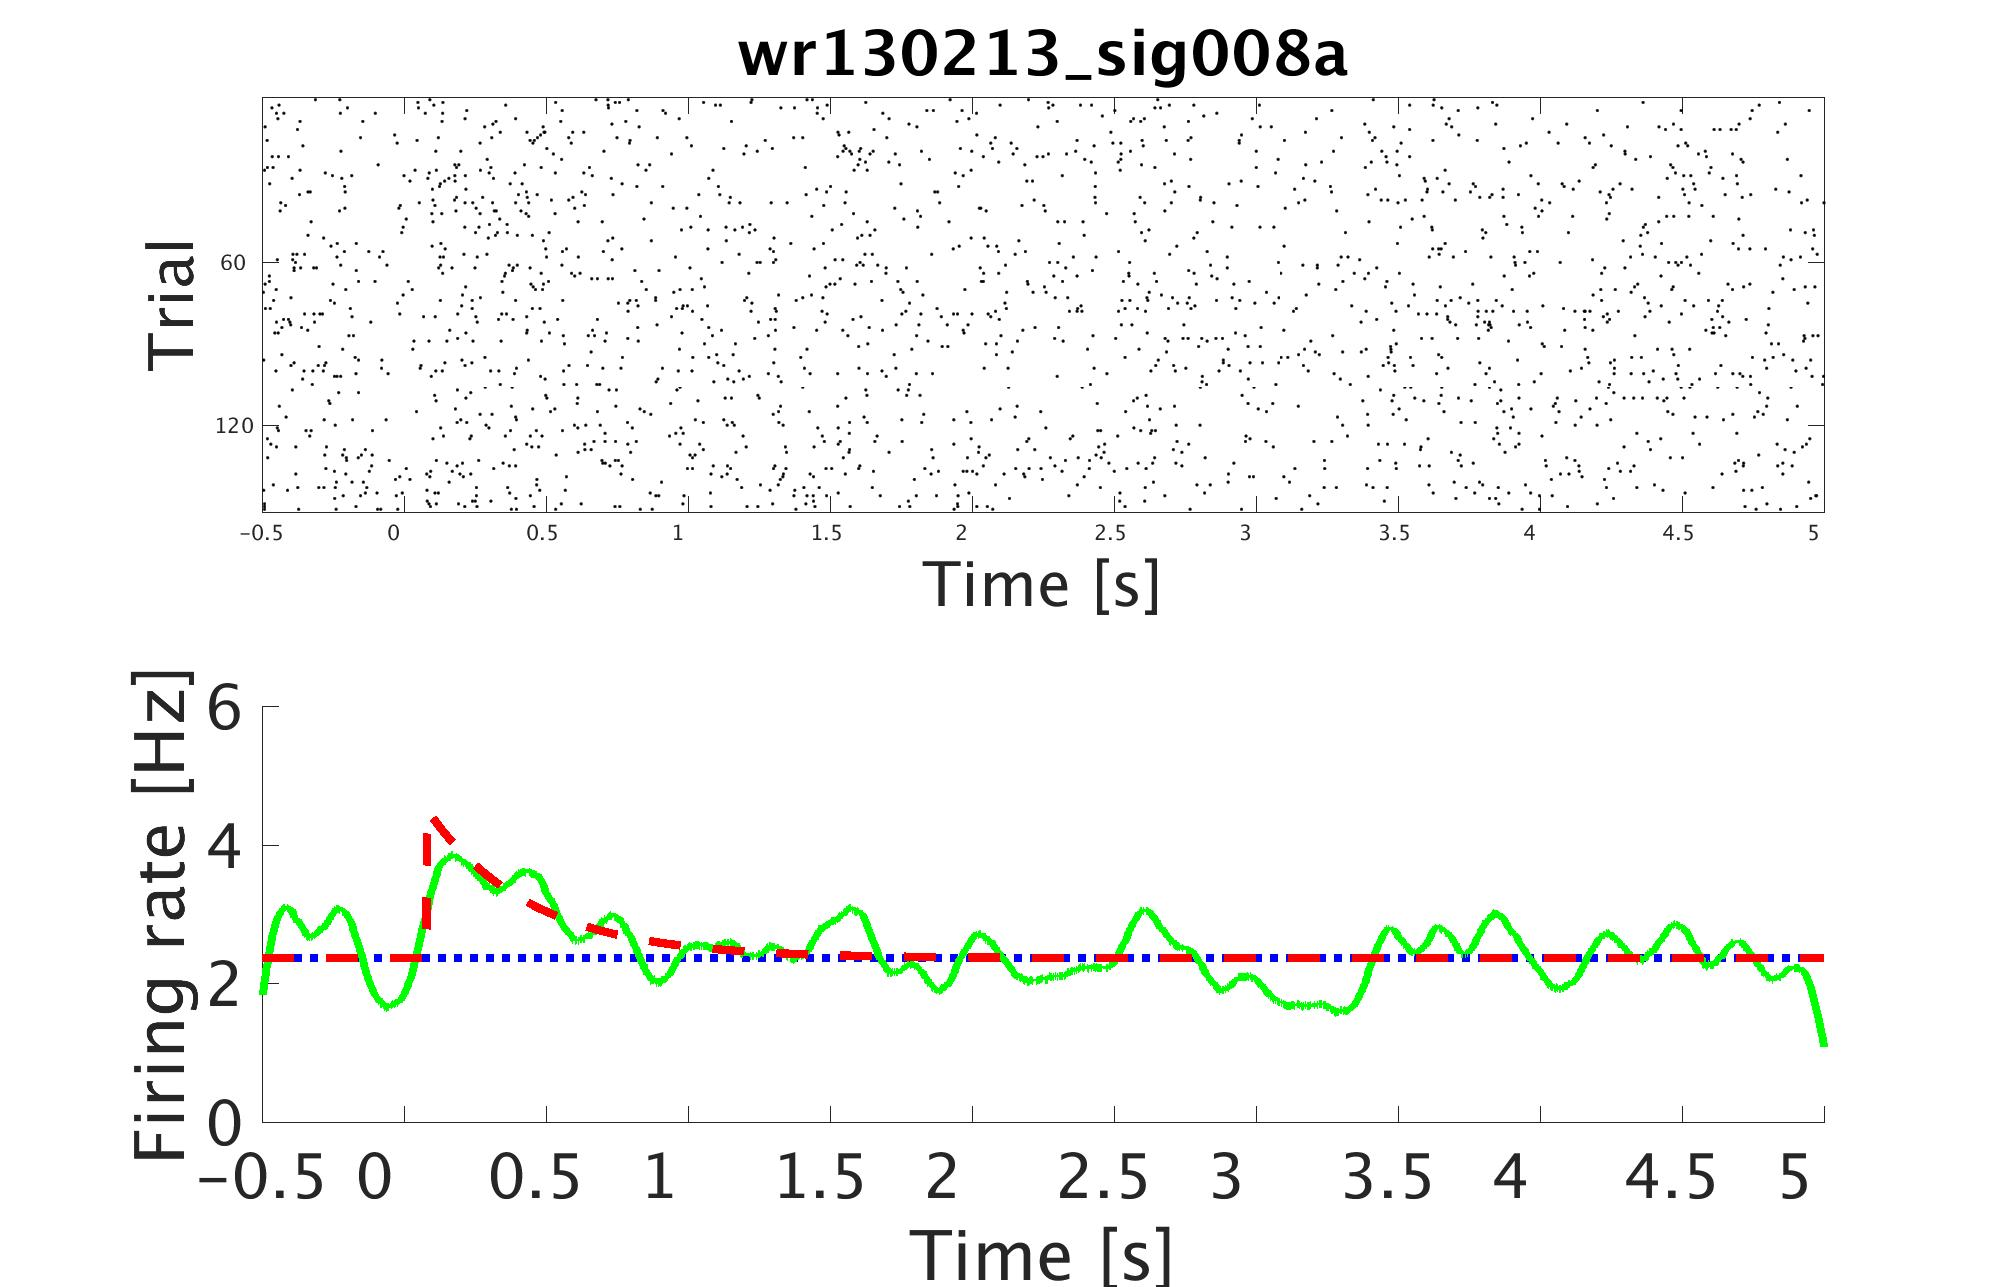
\includegraphics[width =.33\textwidth]{Supplemental_Cells/allcell_17_v_11.jpeg}\\ %0.36


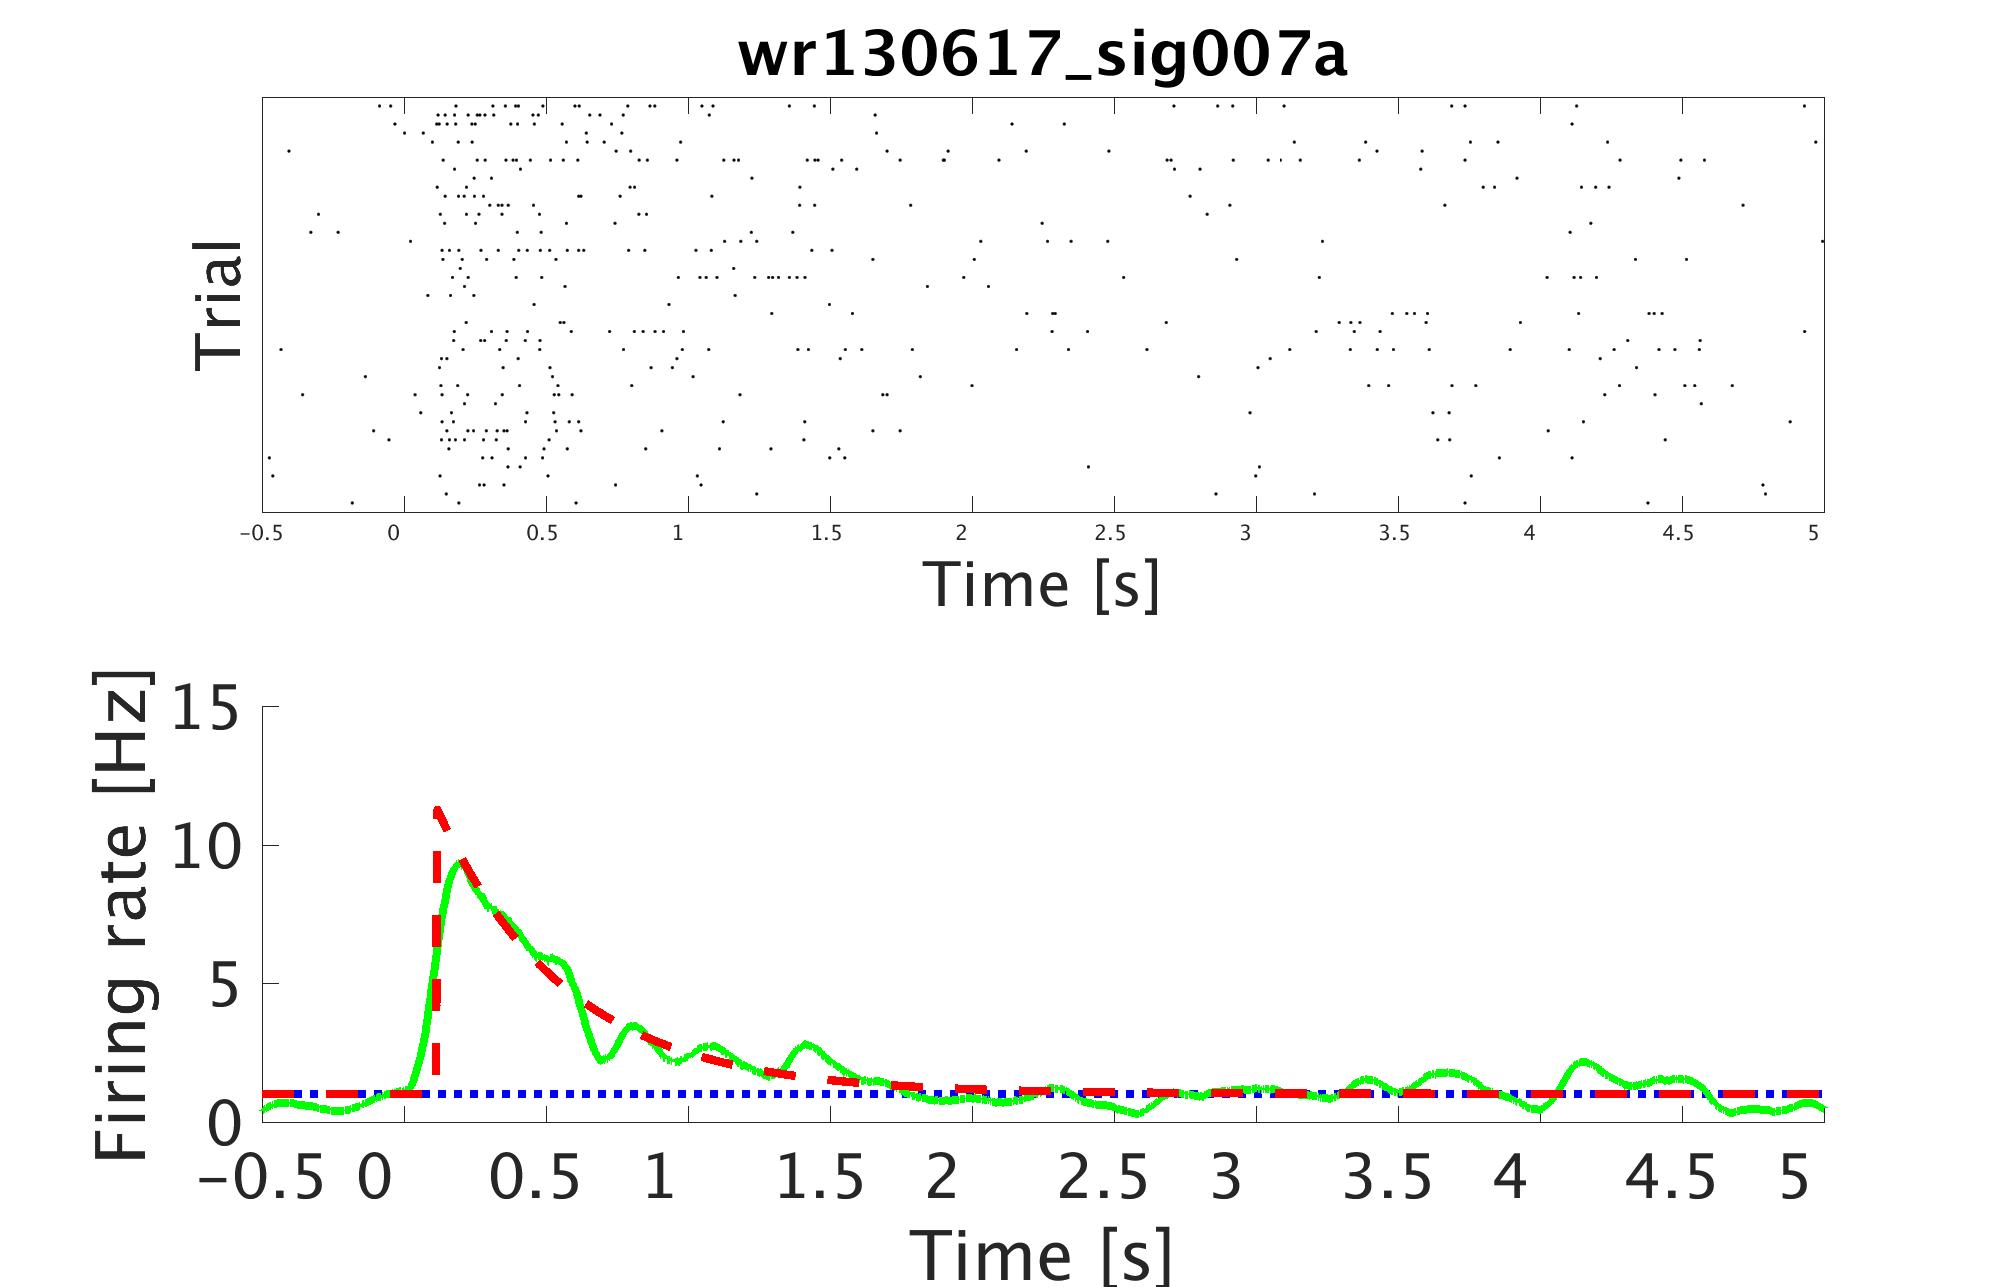
\includegraphics[width =.33\textwidth]{Supplemental_Cells/allcell_209_v_11.jpeg} %0.46
&
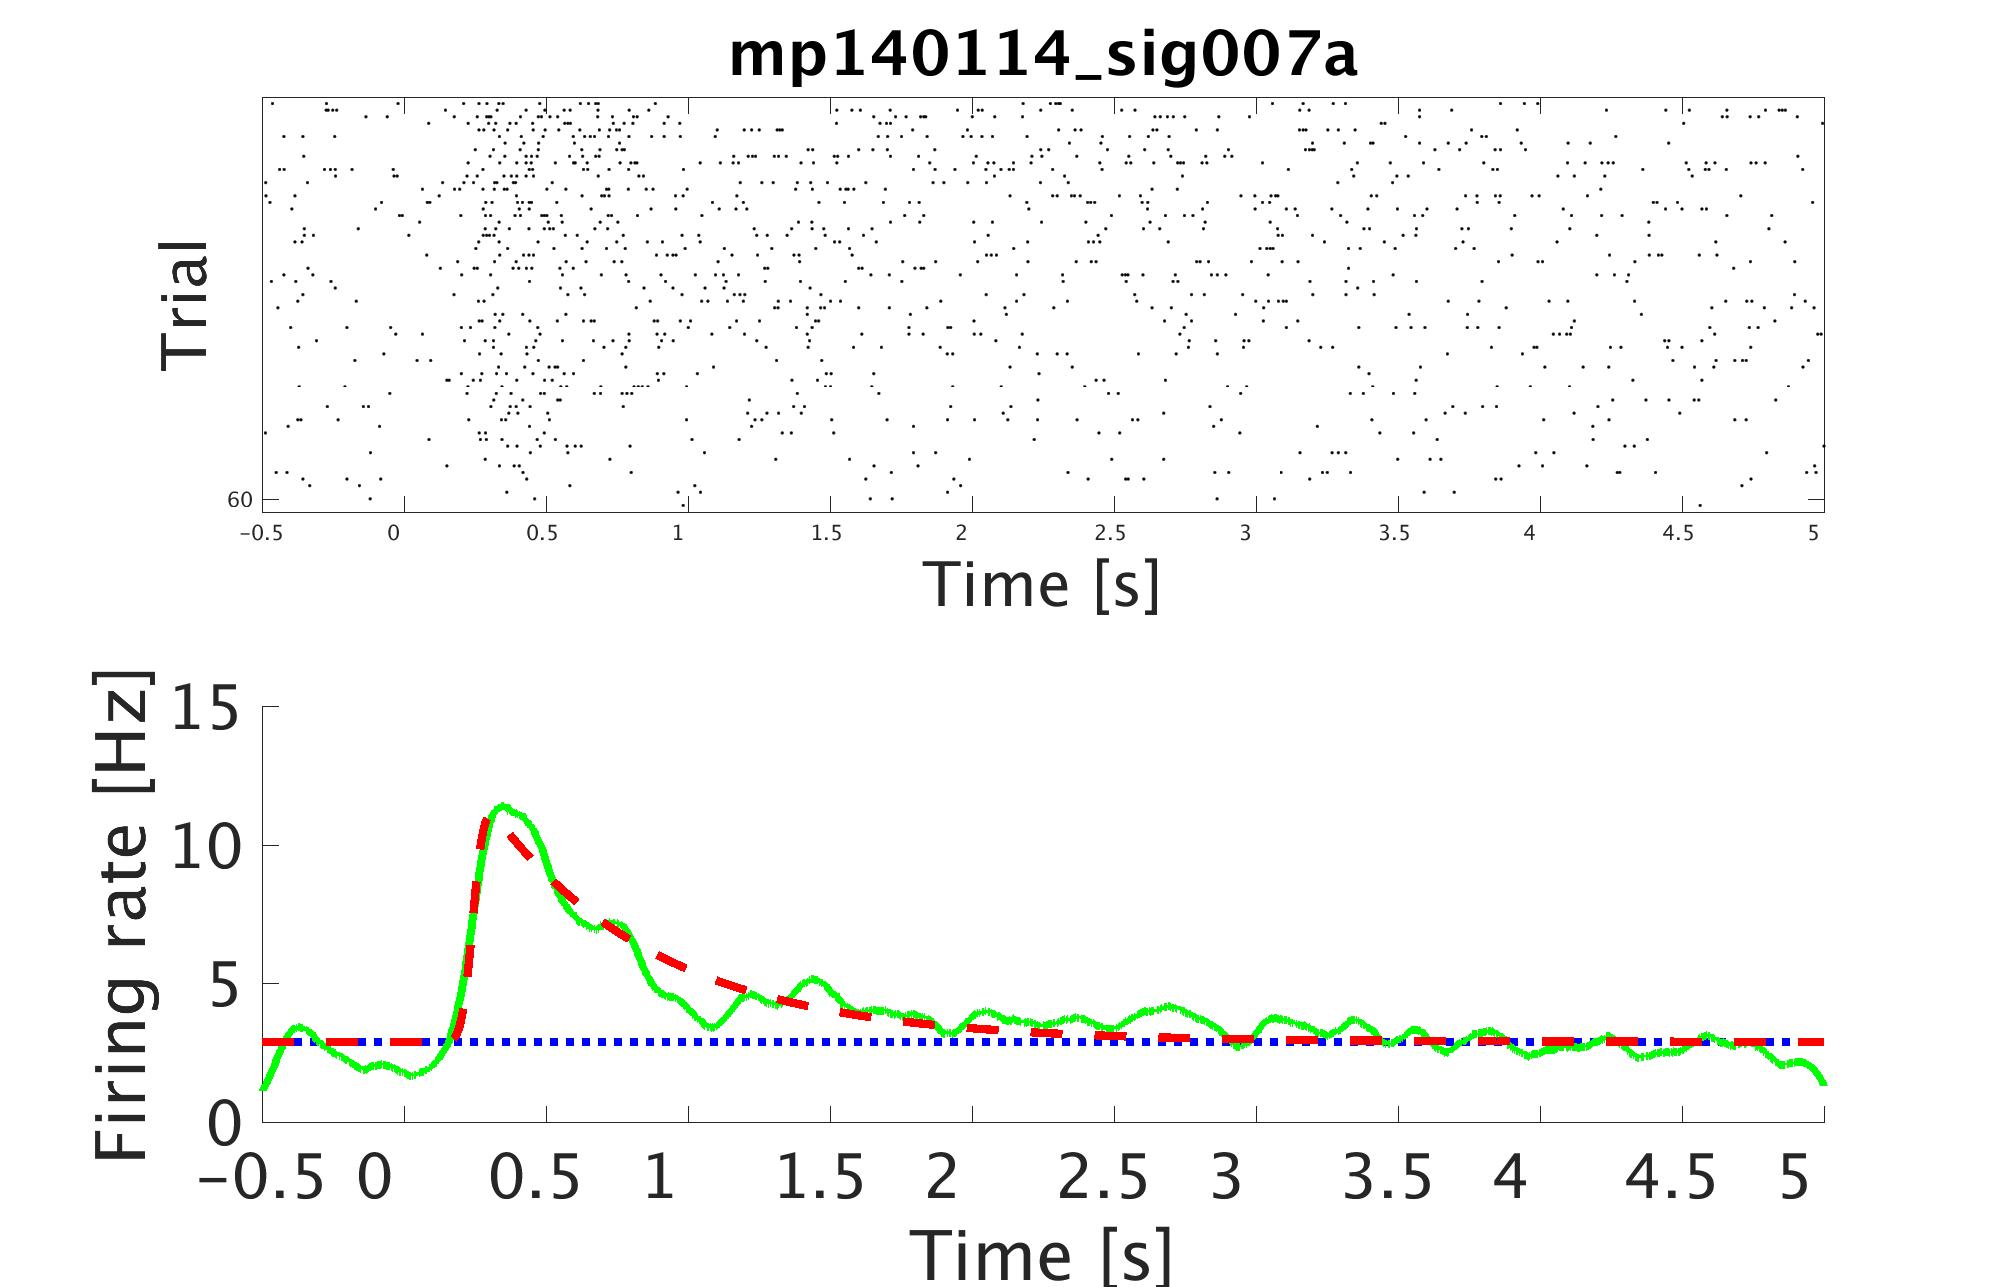
\includegraphics[width =.33\textwidth]{Supplemental_Cells/allcell_252_v_11.jpeg} %0.60
&
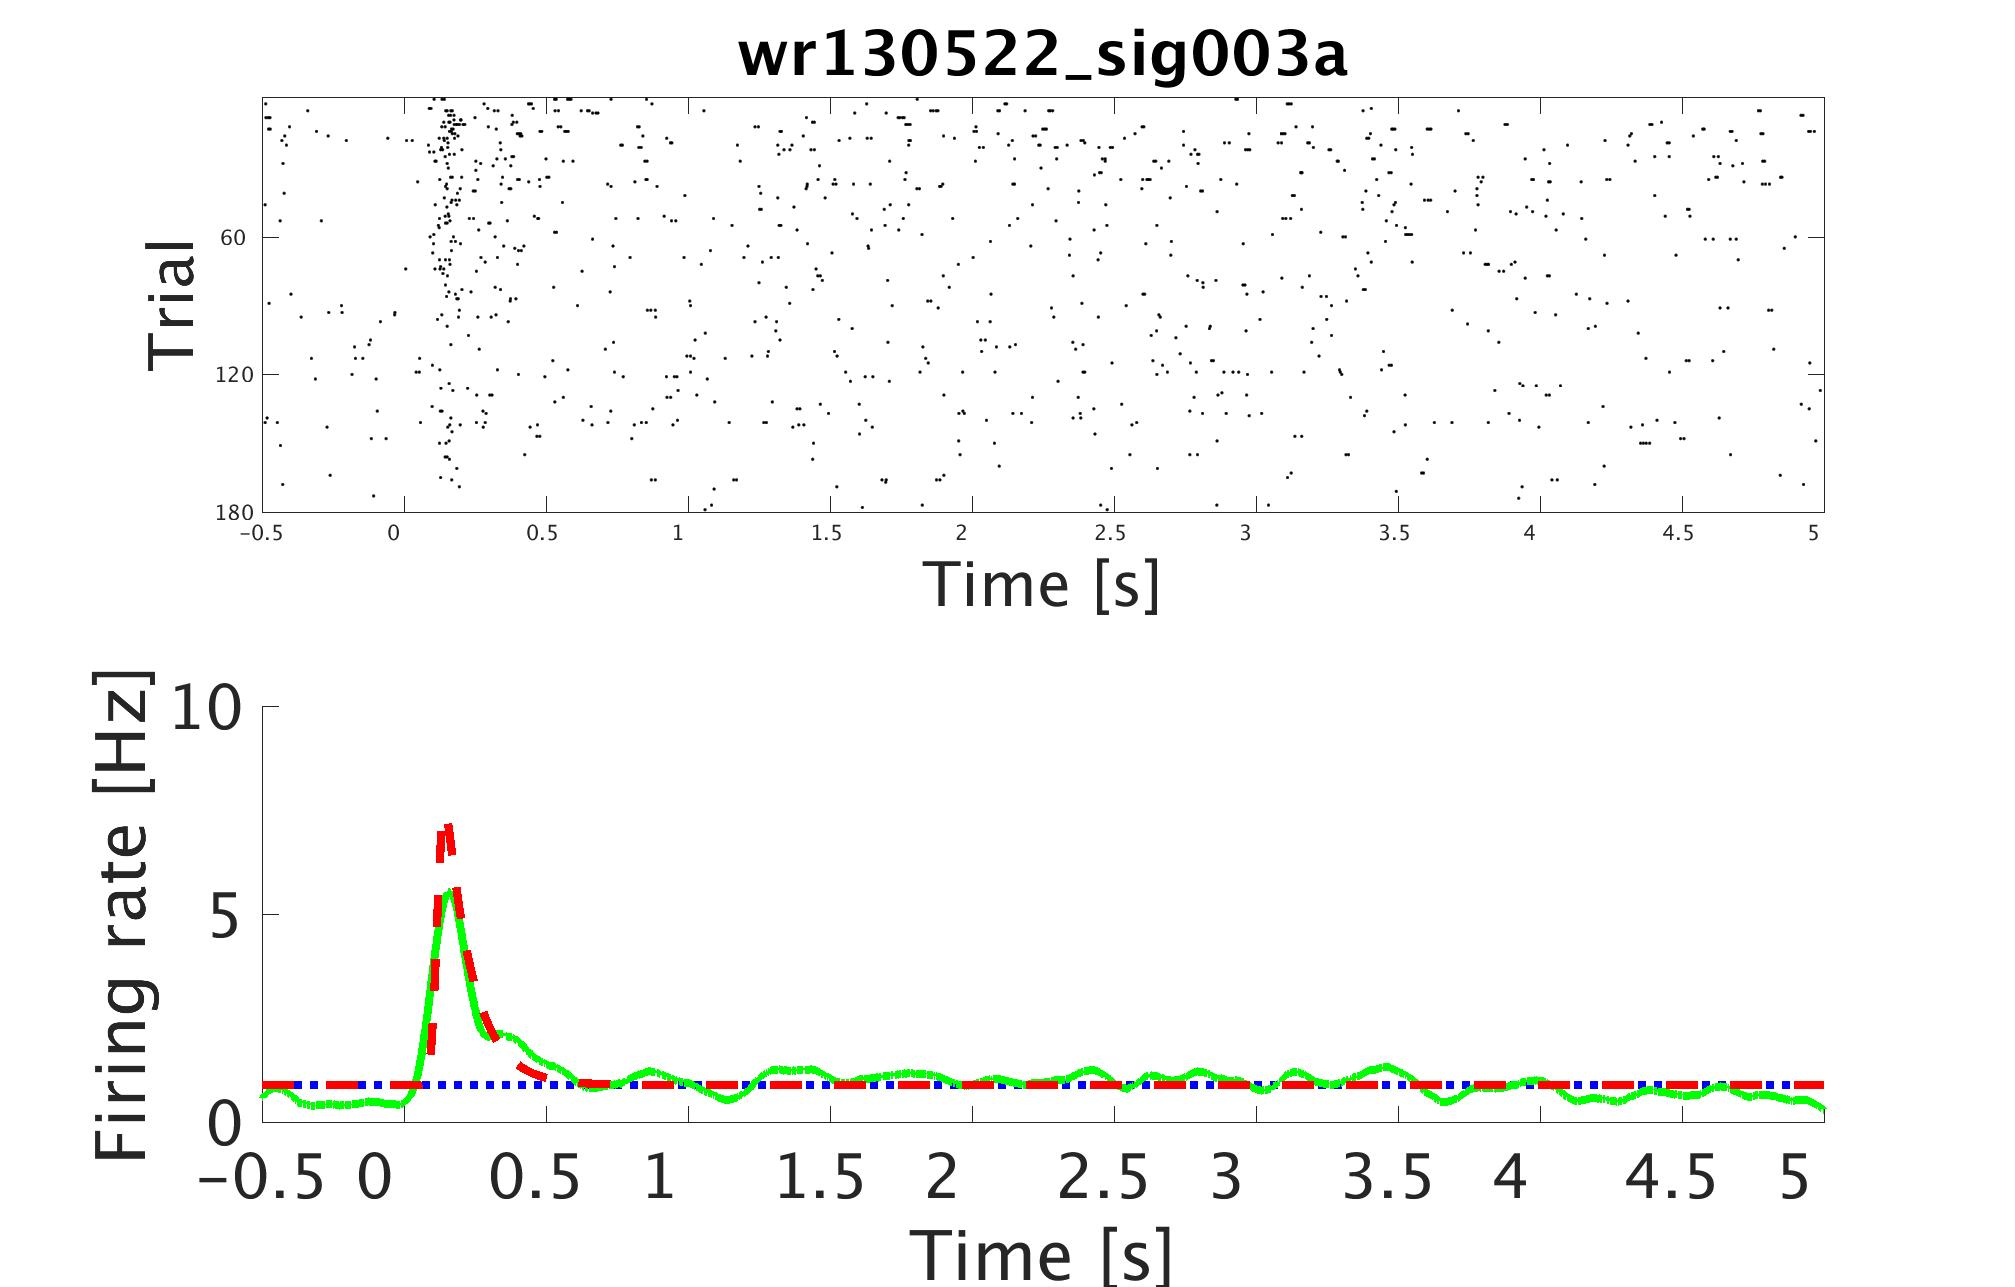
\includegraphics[width =.33\textwidth]{Supplemental_Cells/allcell_137_v_11.jpeg}\\ %0.74


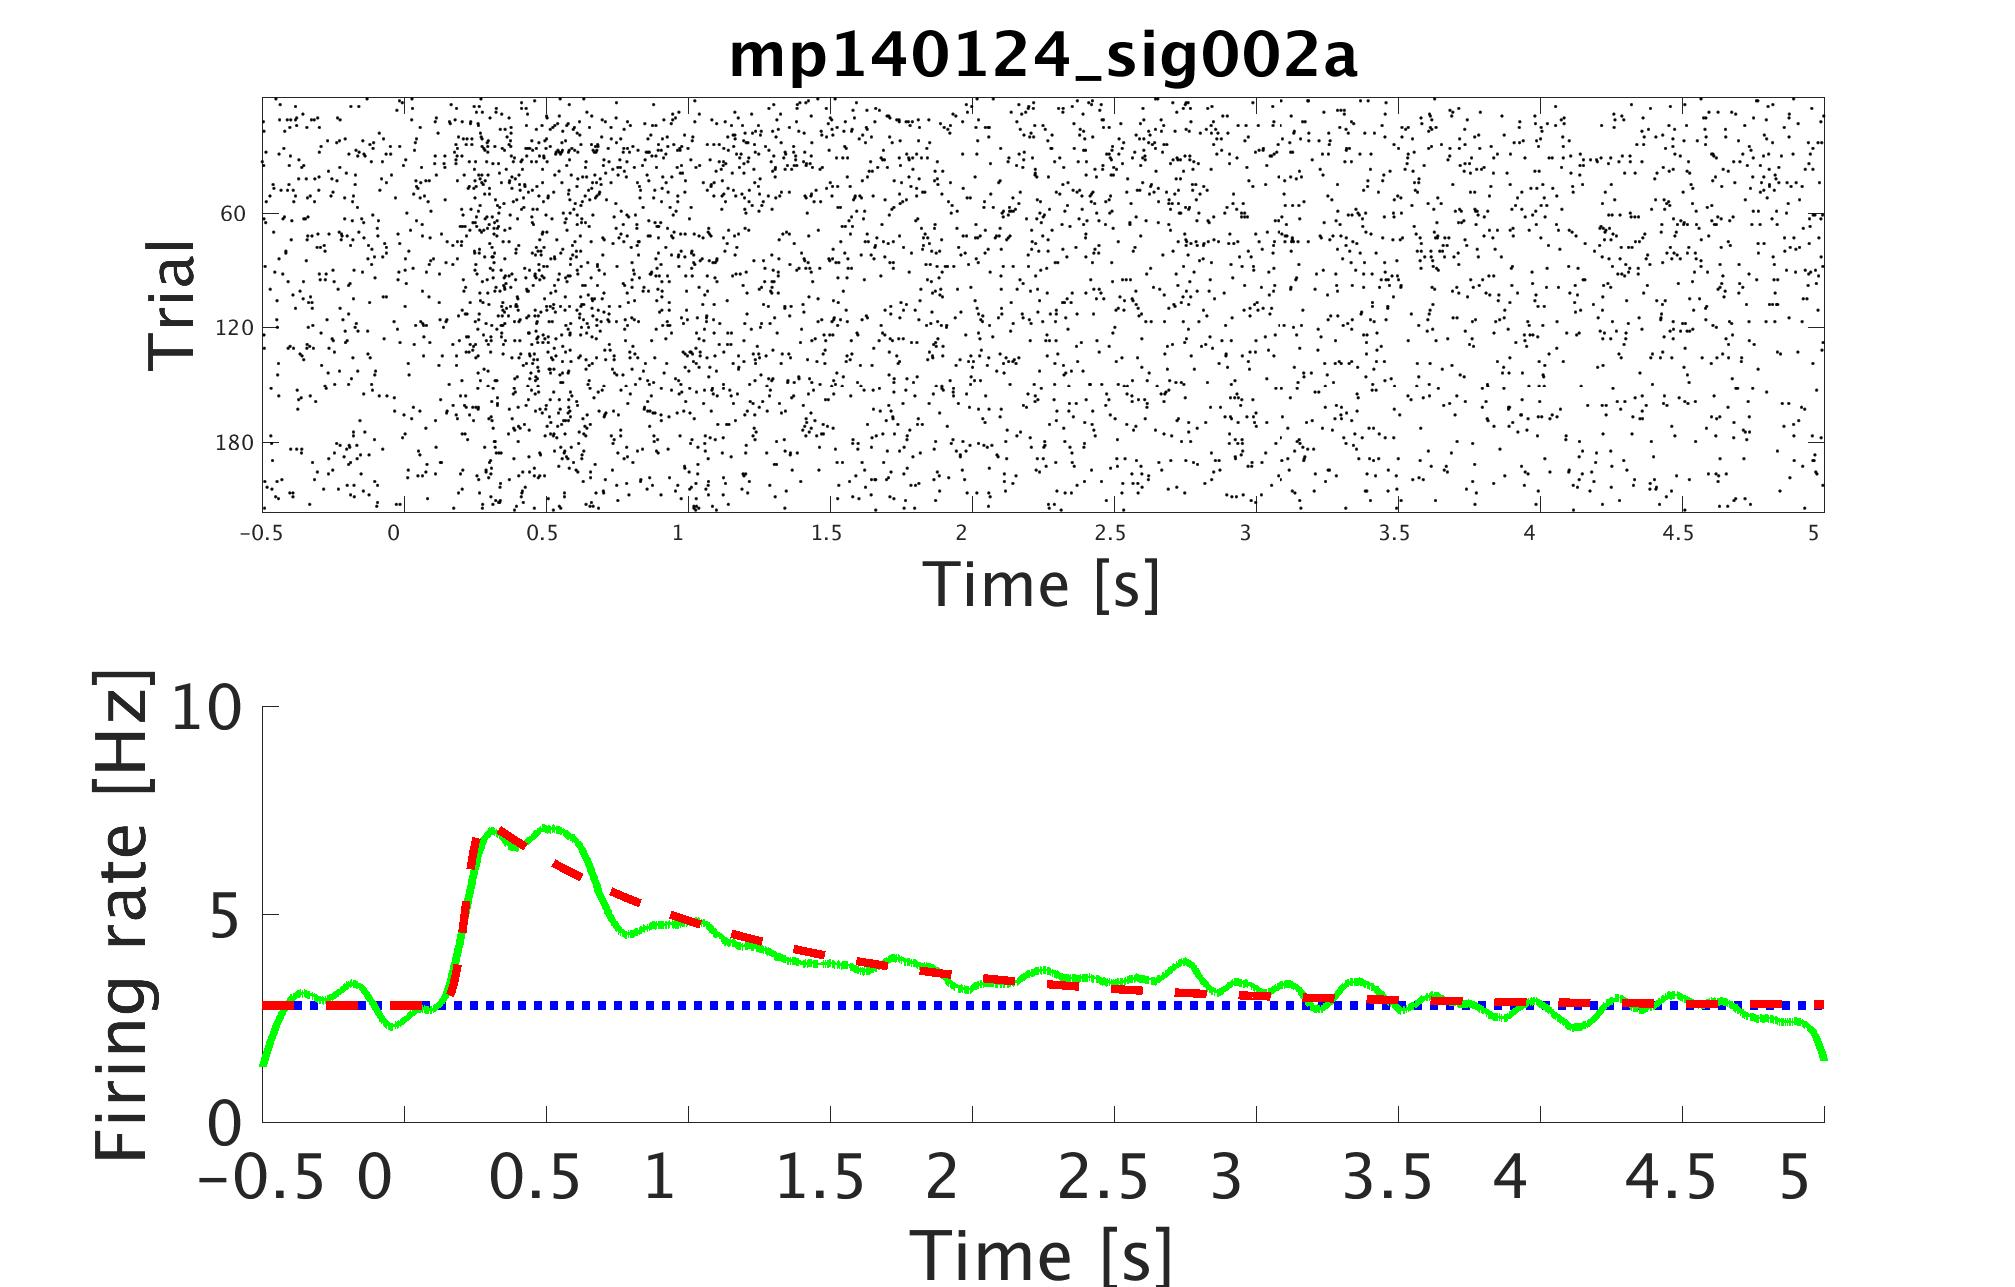
\includegraphics[width =.33\textwidth]{Supplemental_Cells/allcell_289_v_11.jpeg} %0.92
&
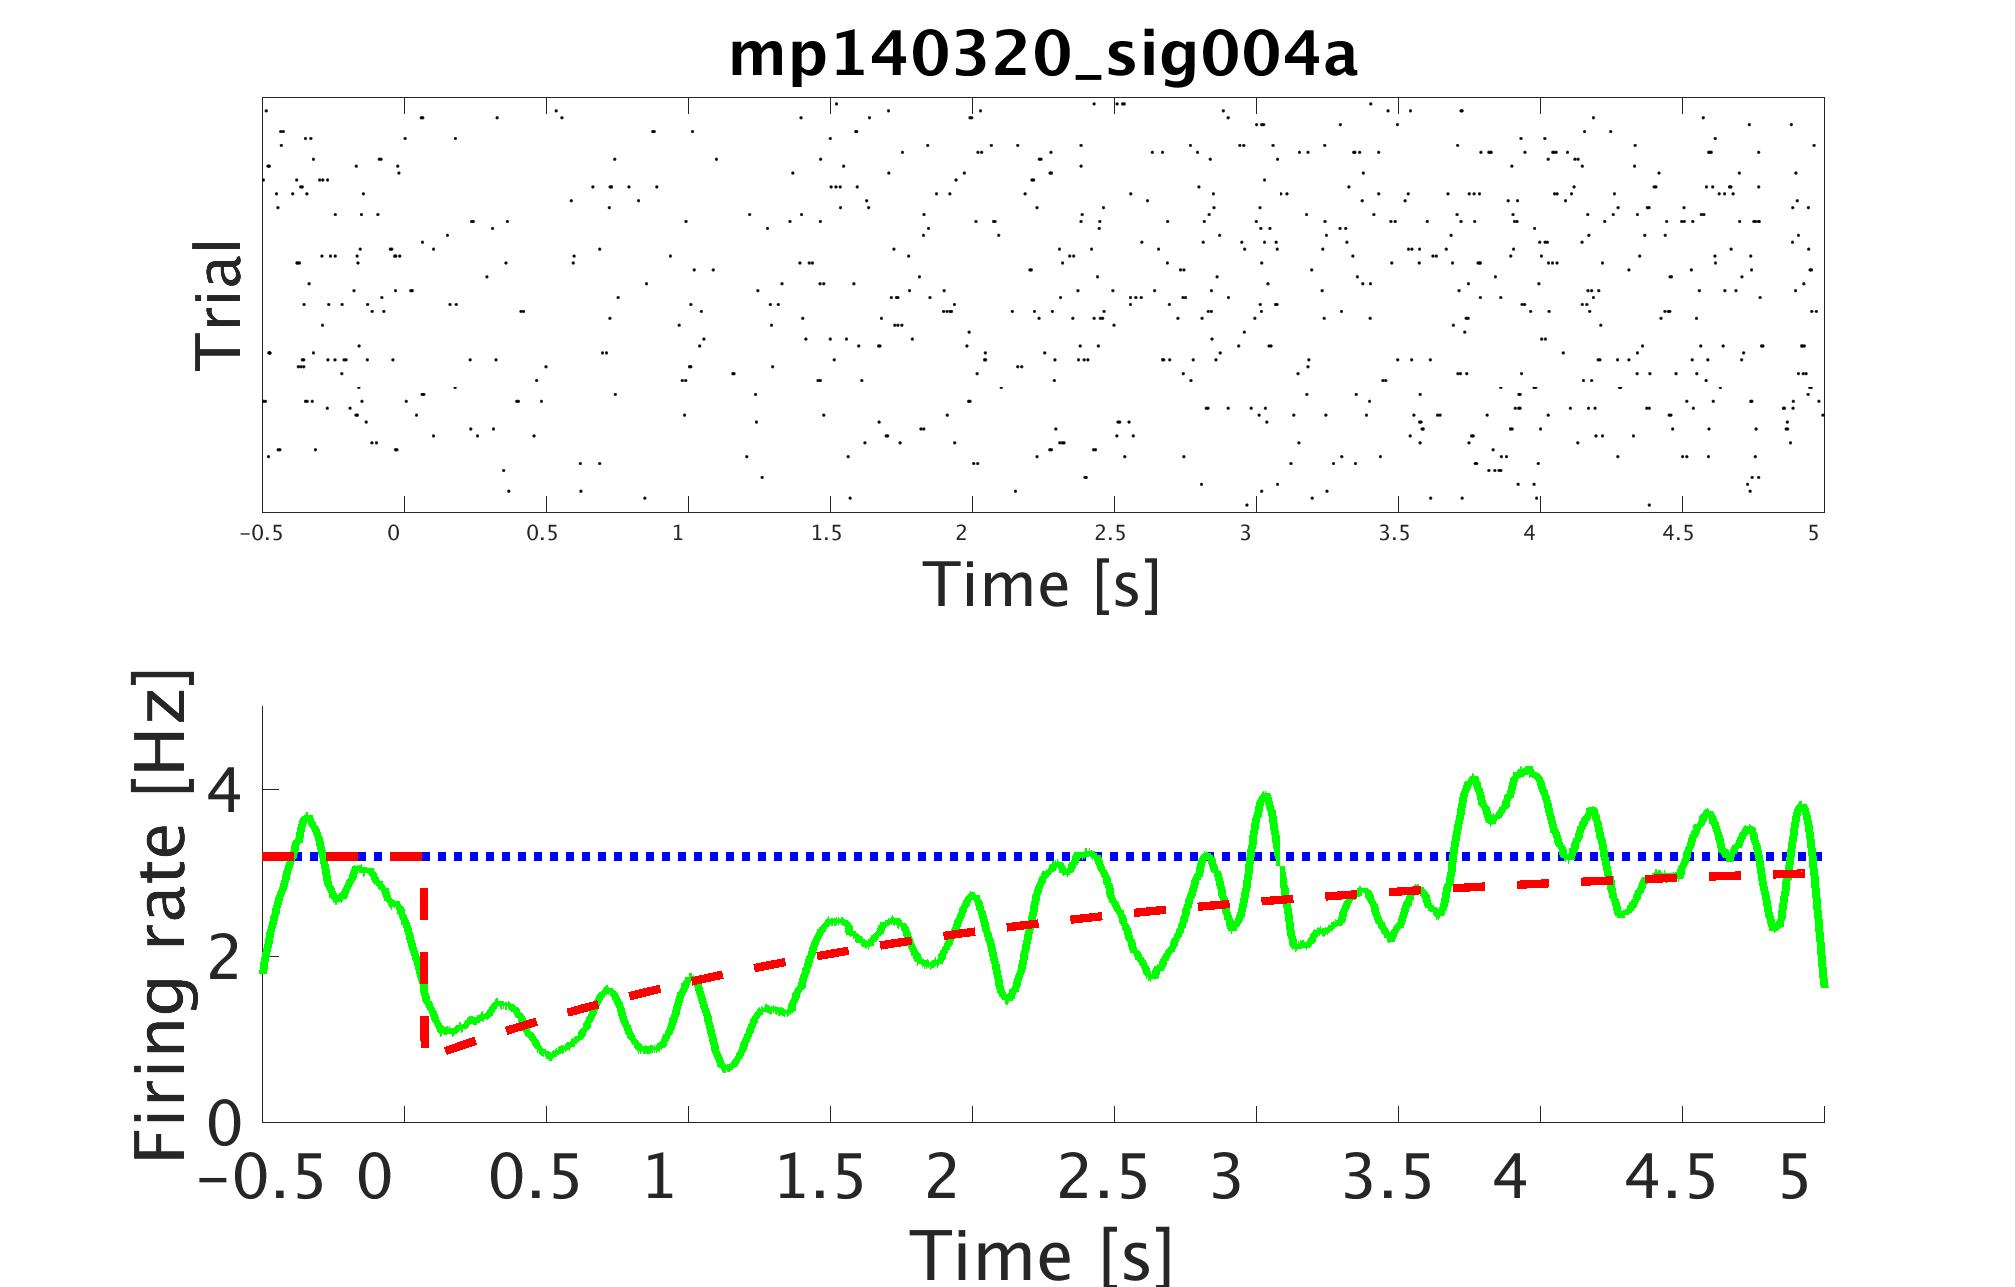
\includegraphics[width =.33\textwidth]{Supplemental_Cells/allcell_330_v_11.jpeg} %1.96
&
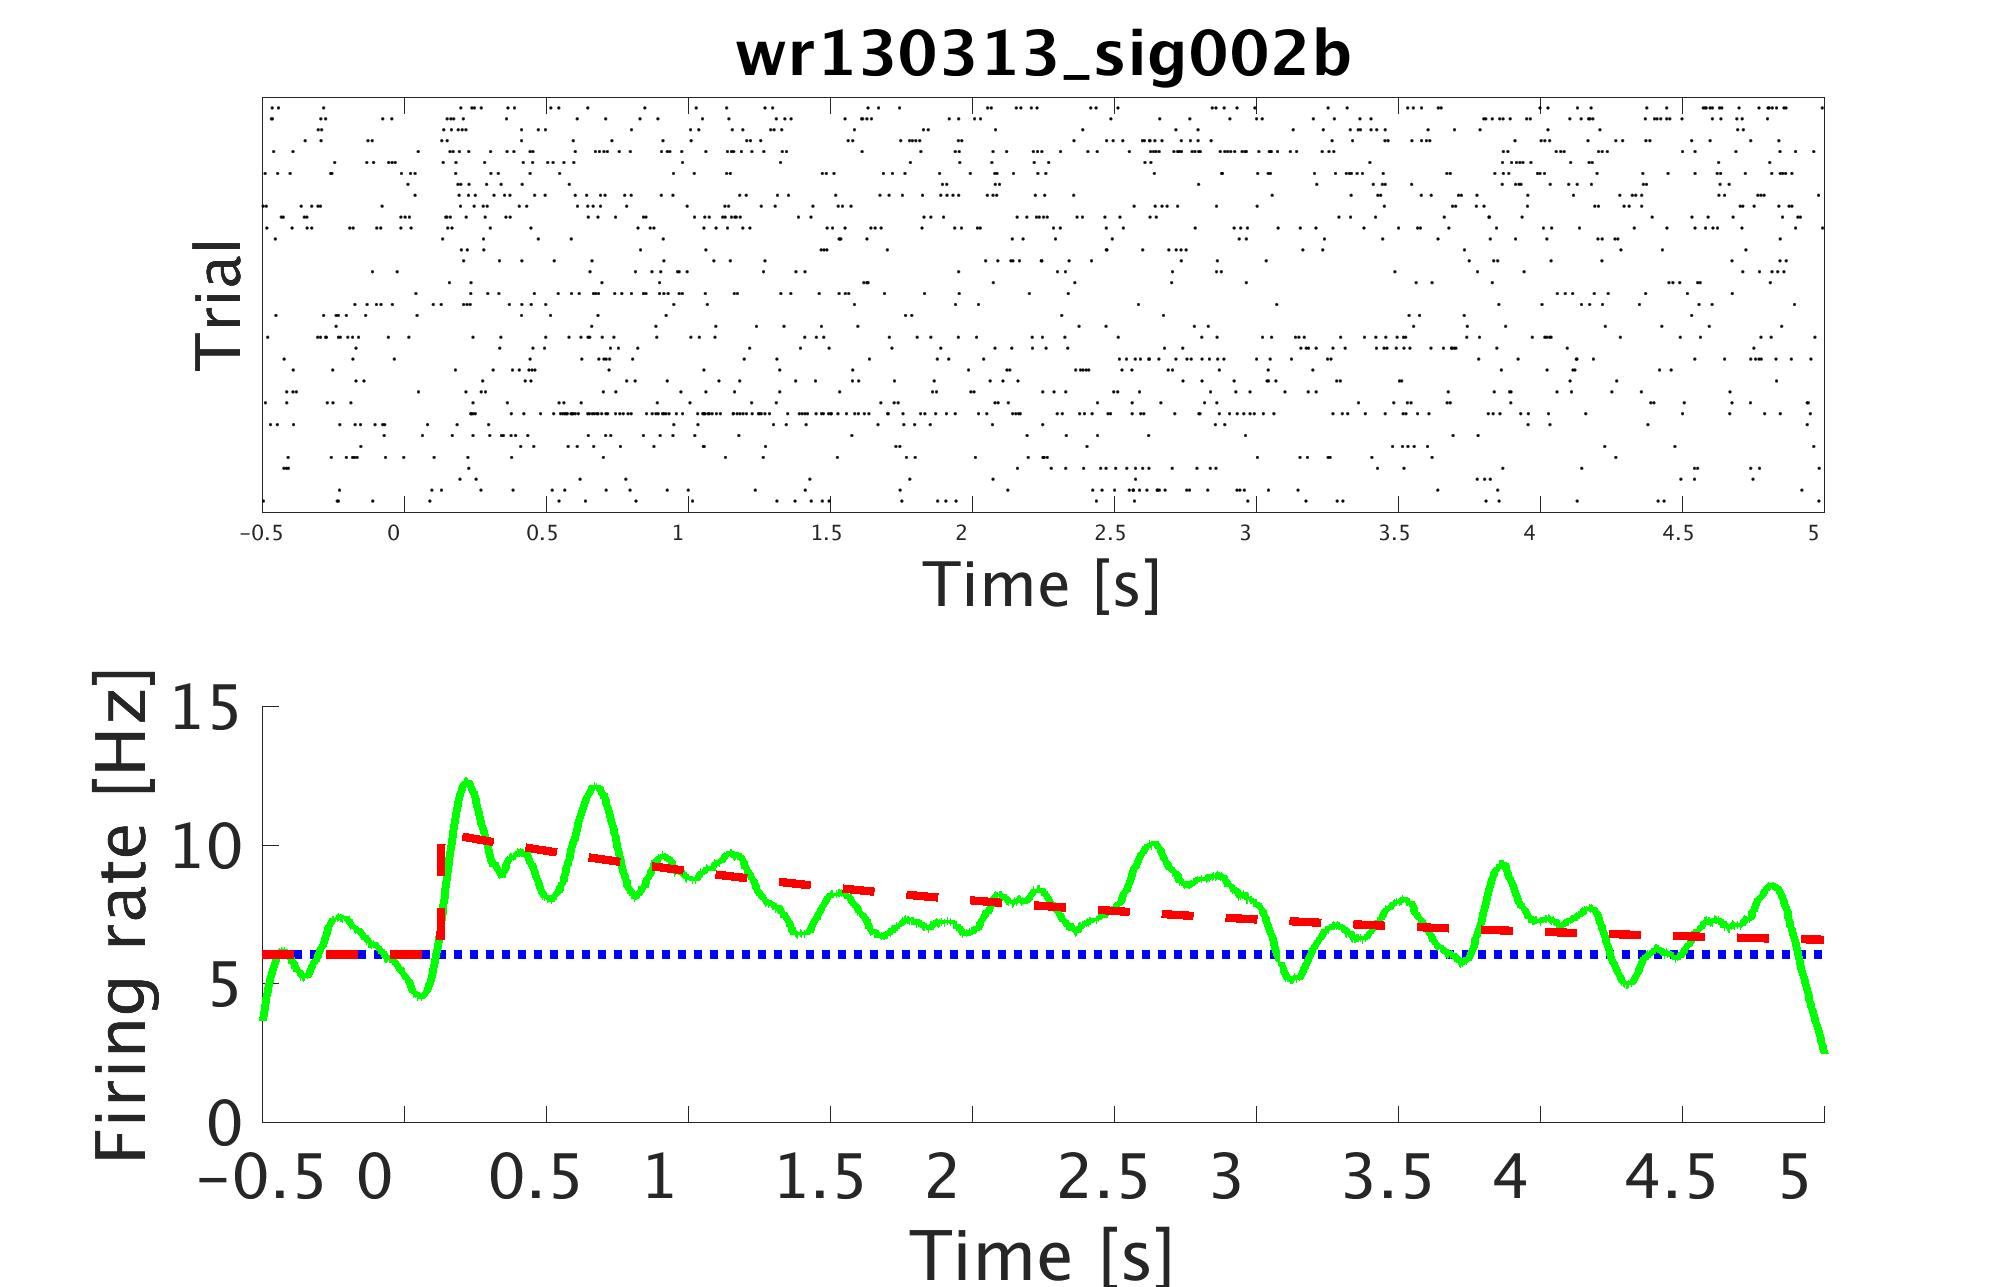
\includegraphics[width =.33\textwidth]{Supplemental_Cells/allcell_123_v_11.jpeg}\\%2.30



\end{tabular}

\caption{ \textbf{Additional examples of temporal context cells.} Format is as
in Figure~\ref{fig:SingleCellResults}a.  Units are ordered by their
estimated relaxation rate ($\tau$).
\label{fig:MoreTCC} 
} 
\end{figure}

\end{document}
